% Options for packages loaded elsewhere
\PassOptionsToPackage{unicode}{hyperref}
\PassOptionsToPackage{hyphens}{url}
%
\documentclass[
]{article}
\usepackage{amsmath,amssymb}
\usepackage{lmodern}
\usepackage{iftex}
\ifPDFTeX
  \usepackage[T1]{fontenc}
  \usepackage[utf8]{inputenc}
  \usepackage{textcomp} % provide euro and other symbols
\else % if luatex or xetex
  \usepackage{unicode-math}
  \defaultfontfeatures{Scale=MatchLowercase}
  \defaultfontfeatures[\rmfamily]{Ligatures=TeX,Scale=1}
\fi
% Use upquote if available, for straight quotes in verbatim environments
\IfFileExists{upquote.sty}{\usepackage{upquote}}{}
\IfFileExists{microtype.sty}{% use microtype if available
  \usepackage[]{microtype}
  \UseMicrotypeSet[protrusion]{basicmath} % disable protrusion for tt fonts
}{}
\makeatletter
\@ifundefined{KOMAClassName}{% if non-KOMA class
  \IfFileExists{parskip.sty}{%
    \usepackage{parskip}
  }{% else
    \setlength{\parindent}{0pt}
    \setlength{\parskip}{6pt plus 2pt minus 1pt}}
}{% if KOMA class
  \KOMAoptions{parskip=half}}
\makeatother
\usepackage{xcolor}
\usepackage[margin=1in]{geometry}
\usepackage{color}
\usepackage{fancyvrb}
\newcommand{\VerbBar}{|}
\newcommand{\VERB}{\Verb[commandchars=\\\{\}]}
\DefineVerbatimEnvironment{Highlighting}{Verbatim}{commandchars=\\\{\}}
% Add ',fontsize=\small' for more characters per line
\usepackage{framed}
\definecolor{shadecolor}{RGB}{248,248,248}
\newenvironment{Shaded}{\begin{snugshade}}{\end{snugshade}}
\newcommand{\AlertTok}[1]{\textcolor[rgb]{0.94,0.16,0.16}{#1}}
\newcommand{\AnnotationTok}[1]{\textcolor[rgb]{0.56,0.35,0.01}{\textbf{\textit{#1}}}}
\newcommand{\AttributeTok}[1]{\textcolor[rgb]{0.77,0.63,0.00}{#1}}
\newcommand{\BaseNTok}[1]{\textcolor[rgb]{0.00,0.00,0.81}{#1}}
\newcommand{\BuiltInTok}[1]{#1}
\newcommand{\CharTok}[1]{\textcolor[rgb]{0.31,0.60,0.02}{#1}}
\newcommand{\CommentTok}[1]{\textcolor[rgb]{0.56,0.35,0.01}{\textit{#1}}}
\newcommand{\CommentVarTok}[1]{\textcolor[rgb]{0.56,0.35,0.01}{\textbf{\textit{#1}}}}
\newcommand{\ConstantTok}[1]{\textcolor[rgb]{0.00,0.00,0.00}{#1}}
\newcommand{\ControlFlowTok}[1]{\textcolor[rgb]{0.13,0.29,0.53}{\textbf{#1}}}
\newcommand{\DataTypeTok}[1]{\textcolor[rgb]{0.13,0.29,0.53}{#1}}
\newcommand{\DecValTok}[1]{\textcolor[rgb]{0.00,0.00,0.81}{#1}}
\newcommand{\DocumentationTok}[1]{\textcolor[rgb]{0.56,0.35,0.01}{\textbf{\textit{#1}}}}
\newcommand{\ErrorTok}[1]{\textcolor[rgb]{0.64,0.00,0.00}{\textbf{#1}}}
\newcommand{\ExtensionTok}[1]{#1}
\newcommand{\FloatTok}[1]{\textcolor[rgb]{0.00,0.00,0.81}{#1}}
\newcommand{\FunctionTok}[1]{\textcolor[rgb]{0.00,0.00,0.00}{#1}}
\newcommand{\ImportTok}[1]{#1}
\newcommand{\InformationTok}[1]{\textcolor[rgb]{0.56,0.35,0.01}{\textbf{\textit{#1}}}}
\newcommand{\KeywordTok}[1]{\textcolor[rgb]{0.13,0.29,0.53}{\textbf{#1}}}
\newcommand{\NormalTok}[1]{#1}
\newcommand{\OperatorTok}[1]{\textcolor[rgb]{0.81,0.36,0.00}{\textbf{#1}}}
\newcommand{\OtherTok}[1]{\textcolor[rgb]{0.56,0.35,0.01}{#1}}
\newcommand{\PreprocessorTok}[1]{\textcolor[rgb]{0.56,0.35,0.01}{\textit{#1}}}
\newcommand{\RegionMarkerTok}[1]{#1}
\newcommand{\SpecialCharTok}[1]{\textcolor[rgb]{0.00,0.00,0.00}{#1}}
\newcommand{\SpecialStringTok}[1]{\textcolor[rgb]{0.31,0.60,0.02}{#1}}
\newcommand{\StringTok}[1]{\textcolor[rgb]{0.31,0.60,0.02}{#1}}
\newcommand{\VariableTok}[1]{\textcolor[rgb]{0.00,0.00,0.00}{#1}}
\newcommand{\VerbatimStringTok}[1]{\textcolor[rgb]{0.31,0.60,0.02}{#1}}
\newcommand{\WarningTok}[1]{\textcolor[rgb]{0.56,0.35,0.01}{\textbf{\textit{#1}}}}
\usepackage{graphicx}
\makeatletter
\def\maxwidth{\ifdim\Gin@nat@width>\linewidth\linewidth\else\Gin@nat@width\fi}
\def\maxheight{\ifdim\Gin@nat@height>\textheight\textheight\else\Gin@nat@height\fi}
\makeatother
% Scale images if necessary, so that they will not overflow the page
% margins by default, and it is still possible to overwrite the defaults
% using explicit options in \includegraphics[width, height, ...]{}
\setkeys{Gin}{width=\maxwidth,height=\maxheight,keepaspectratio}
% Set default figure placement to htbp
\makeatletter
\def\fps@figure{htbp}
\makeatother
\setlength{\emergencystretch}{3em} % prevent overfull lines
\providecommand{\tightlist}{%
  \setlength{\itemsep}{0pt}\setlength{\parskip}{0pt}}
\setcounter{secnumdepth}{-\maxdimen} % remove section numbering
\usepackage{booktabs}
\usepackage{longtable}
\usepackage{array}
\usepackage{multirow}
\usepackage{wrapfig}
\usepackage{float}
\usepackage{colortbl}
\usepackage{pdflscape}
\usepackage{tabu}
\usepackage{threeparttable}
\usepackage{threeparttablex}
\usepackage[normalem]{ulem}
\usepackage{makecell}
\usepackage{xcolor}
\ifLuaTeX
  \usepackage{selnolig}  % disable illegal ligatures
\fi
\IfFileExists{bookmark.sty}{\usepackage{bookmark}}{\usepackage{hyperref}}
\IfFileExists{xurl.sty}{\usepackage{xurl}}{} % add URL line breaks if available
\urlstyle{same} % disable monospaced font for URLs
\hypersetup{
  pdftitle={Project},
  pdfauthor={B203349},
  hidelinks,
  pdfcreator={LaTeX via pandoc}}

\title{Project}
\author{B203349}
\date{2022-12-11}

\begin{document}
\maketitle

{
\setcounter{tocdepth}{2}
\tableofcontents
}
\hypertarget{click-here-to-link-to-my-gpresentation}{%
\section{\texorpdfstring{\href{https://github.com/B203349/B203349_assessment}{Click
here to link to my
gpresentation}}{Click here to link to my gpresentation}}\label{click-here-to-link-to-my-gpresentation}}

\hypertarget{loading-the-required-packages-required-for-this-script}{%
\section{Loading the required packages required for this
script}\label{loading-the-required-packages-required-for-this-script}}

\begin{Shaded}
\begin{Highlighting}[]
\FunctionTok{library}\NormalTok{(sparklyr)}
\FunctionTok{library}\NormalTok{(dplyr)}
\FunctionTok{library}\NormalTok{(ggplot2)}
\FunctionTok{library}\NormalTok{(cowplot)}
\FunctionTok{library}\NormalTok{(knitr)}
\FunctionTok{library}\NormalTok{(kableExtra)}
\FunctionTok{library}\NormalTok{(tidyverse) }
\FunctionTok{library}\NormalTok{(lubridate) }
\FunctionTok{library}\NormalTok{(ggplot2)}
\FunctionTok{library}\NormalTok{(dbplot)}
\FunctionTok{library}\NormalTok{(janitor)}
\FunctionTok{library}\NormalTok{(broom)}
\FunctionTok{library}\NormalTok{(formatR)}
\end{Highlighting}
\end{Shaded}

\hypertarget{connecting-to-spark-in-local-mode}{%
\subsection{Connecting to Spark in local
mode}\label{connecting-to-spark-in-local-mode}}

\begin{Shaded}
\begin{Highlighting}[]
\NormalTok{sc }\OtherTok{=} \FunctionTok{spark\_connect}\NormalTok{(}\AttributeTok{master =} \StringTok{\textquotesingle{}local\textquotesingle{}}\NormalTok{)}
\end{Highlighting}
\end{Shaded}

\hypertarget{loading-datasets}{%
\section{Loading datasets}\label{loading-datasets}}

\hypertarget{data}{%
\subsection{Data}\label{data}}

The \textbf{Diabetes 130-US hospitals for years 1999-2008 Data Set} is
an extract representing 10 years (1999--2008) of clinical care at 130
hospitals and integrated delivery networks throughout the United States.
The dataset was compiled Strack et al{[}1{]} and is in .csv format.

\hypertarget{read-.csv-downloaded-from-and-create-dataframe}{%
\subsection{Read .csv downloaded from and create
dataframe}\label{read-.csv-downloaded-from-and-create-dataframe}}

\begin{Shaded}
\begin{Highlighting}[]
\CommentTok{\# diabetic\_data =}
\CommentTok{\# spark\_read\_csv(sc,}
\CommentTok{\# \textquotesingle{}/Users/matt/Desktop/Dropbox/Home/College/Edinburgh}
\CommentTok{\# {-} MSc Data Science/Big}
\CommentTok{\# Data}
\CommentTok{\# Analytics/diabetes\_readmissions/RawData/diabetic\_data.csv\textquotesingle{})}
\NormalTok{diabetic\_data }\OtherTok{=} \FunctionTok{spark\_read\_csv}\NormalTok{(sc,}
    \StringTok{"/home/jovyan/Matt/diabetes\_readmissions/RawData/diabetic\_data.csv"}\NormalTok{)}
\end{Highlighting}
\end{Shaded}

\hypertarget{exploratory-analysis}{%
\section{Exploratory analysis}\label{exploratory-analysis}}

\hypertarget{summary-of-data}{%
\subsection{Summary of data}\label{summary-of-data}}

The dataset contains over 50 variables, broadly these describe: patient
demographics, patient diagnoses, admission and discharge dispositions,
length of stay, blood glucose levels, medication types and changes, and
readmission data. Furthermore, procedures, medications, and outpatient /
inpatient / ED visits are all also quantified. The full list of
variables is outlined below:

\begin{Shaded}
\begin{Highlighting}[]
\FunctionTok{glimpse}\NormalTok{(diabetic\_data)}
\end{Highlighting}
\end{Shaded}

\begin{verbatim}
## Rows: ??
## Columns: 50
## Database: spark_connection
## $ encounter_id             <int> 2278392, 149190, 64410, 500364, 16680, 35754,~
## $ patient_nbr              <int> 8222157, 55629189, 86047875, 82442376, 425192~
## $ race                     <chr> "Caucasian", "Caucasian", "AfricanAmerican", ~
## $ gender                   <chr> "Female", "Female", "Female", "Male", "Male",~
## $ age                      <chr> "[0-10)", "[10-20)", "[20-30)", "[30-40)", "[~
## $ weight                   <chr> "?", "?", "?", "?", "?", "?", "?", "?", "?", ~
## $ admission_type_id        <int> 6, 1, 1, 1, 1, 2, 3, 1, 2, 3, 1, 2, 1, 1, 3, ~
## $ discharge_disposition_id <int> 25, 1, 1, 1, 1, 1, 1, 1, 1, 3, 1, 1, 3, 6, 1,~
## $ admission_source_id      <int> 1, 7, 7, 7, 7, 2, 2, 7, 4, 4, 7, 4, 7, 7, 2, ~
## $ time_in_hospital         <int> 1, 3, 2, 2, 1, 3, 4, 5, 13, 12, 9, 7, 7, 10, ~
## $ payer_code               <chr> "?", "?", "?", "?", "?", "?", "?", "?", "?", ~
## $ medical_specialty        <chr> "Pediatrics-Endocrinology", "?", "?", "?", "?~
## $ num_lab_procedures       <int> 41, 59, 11, 44, 51, 31, 70, 73, 68, 33, 47, 6~
## $ num_procedures           <int> 0, 0, 5, 1, 0, 6, 1, 0, 2, 3, 2, 0, 0, 1, 5, ~
## $ num_medications          <int> 1, 18, 13, 16, 8, 16, 21, 12, 28, 18, 17, 11,~
## $ number_outpatient        <int> 0, 0, 2, 0, 0, 0, 0, 0, 0, 0, 0, 0, 0, 0, 0, ~
## $ number_emergency         <int> 0, 0, 0, 0, 0, 0, 0, 0, 0, 0, 0, 0, 1, 0, 0, ~
## $ number_inpatient         <int> 0, 0, 1, 0, 0, 0, 0, 0, 0, 0, 0, 0, 0, 0, 0, ~
## $ diag_1                   <chr> "250.83", "276", "648", "8", "197", "414", "4~
## $ diag_2                   <chr> "?", "250.01", "250", "250.43", "157", "411",~
## $ diag_3                   <chr> "?", "255", "V27", "403", "250", "250", "V45"~
## $ number_diagnoses         <int> 1, 9, 6, 7, 5, 9, 7, 8, 8, 8, 9, 7, 8, 8, 8, ~
## $ max_glu_serum            <chr> "None", "None", "None", "None", "None", "None~
## $ A1Cresult                <chr> "None", "None", "None", "None", "None", "None~
## $ metformin                <chr> "No", "No", "No", "No", "No", "No", "Steady",~
## $ repaglinide              <chr> "No", "No", "No", "No", "No", "No", "No", "No~
## $ nateglinide              <chr> "No", "No", "No", "No", "No", "No", "No", "No~
## $ chlorpropamide           <chr> "No", "No", "No", "No", "No", "No", "No", "No~
## $ glimepiride              <chr> "No", "No", "No", "No", "No", "No", "Steady",~
## $ acetohexamide            <chr> "No", "No", "No", "No", "No", "No", "No", "No~
## $ glipizide                <chr> "No", "No", "Steady", "No", "Steady", "No", "~
## $ glyburide                <chr> "No", "No", "No", "No", "No", "No", "No", "St~
## $ tolbutamide              <chr> "No", "No", "No", "No", "No", "No", "No", "No~
## $ pioglitazone             <chr> "No", "No", "No", "No", "No", "No", "No", "No~
## $ rosiglitazone            <chr> "No", "No", "No", "No", "No", "No", "No", "No~
## $ acarbose                 <chr> "No", "No", "No", "No", "No", "No", "No", "No~
## $ miglitol                 <chr> "No", "No", "No", "No", "No", "No", "No", "No~
## $ troglitazone             <chr> "No", "No", "No", "No", "No", "No", "No", "No~
## $ tolazamide               <chr> "No", "No", "No", "No", "No", "No", "No", "No~
## $ examide                  <chr> "No", "No", "No", "No", "No", "No", "No", "No~
## $ citoglipton              <chr> "No", "No", "No", "No", "No", "No", "No", "No~
## $ insulin                  <chr> "No", "Up", "No", "Up", "Steady", "Steady", "~
## $ glyburidemetformin       <chr> "No", "No", "No", "No", "No", "No", "No", "No~
## $ glipizidemetformin       <chr> "No", "No", "No", "No", "No", "No", "No", "No~
## $ glimepiridepioglitazone  <chr> "No", "No", "No", "No", "No", "No", "No", "No~
## $ metforminrosiglitazone   <chr> "No", "No", "No", "No", "No", "No", "No", "No~
## $ metforminpioglitazone    <chr> "No", "No", "No", "No", "No", "No", "No", "No~
## $ change                   <chr> "No", "Ch", "No", "Ch", "Ch", "No", "Ch", "No~
## $ diabetesMed              <chr> "No", "Yes", "Yes", "Yes", "Yes", "Yes", "Yes~
## $ readmitted               <chr> "NO", ">30", "NO", "NO", "NO", ">30", "NO", "~
\end{verbatim}

\hypertarget{data-cleaning-exploration-and-feature-engineering}{%
\section{Data cleaning, exploration, and feature
engineering}\label{data-cleaning-exploration-and-feature-engineering}}

\hypertarget{conversion-of-to-na}{%
\subsection{Conversion of `?' to NA}\label{conversion-of-to-na}}

From review of the dataframe is a apparent that `?' is used instead of
NA. To faciliate data cleaning and wrangling `?' is switched to NA.

\begin{Shaded}
\begin{Highlighting}[]
\CommentTok{\#replace \textquotesingle{}?\textquotesingle{} with NA}
\NormalTok{diabetic\_data }\OtherTok{\textless{}{-}}\NormalTok{ diabetic\_data }\SpecialCharTok{\%\textgreater{}\%}
  \FunctionTok{mutate}\NormalTok{(}\FunctionTok{across}\NormalTok{(}\FunctionTok{where}\NormalTok{(is.character), }\SpecialCharTok{\textasciitilde{}}\FunctionTok{na\_if}\NormalTok{(., }\StringTok{"?"}\NormalTok{)))}
\end{Highlighting}
\end{Shaded}

\hypertarget{duplicate-patients}{%
\subsection{Duplicate patients}\label{duplicate-patients}}

\begin{Shaded}
\begin{Highlighting}[]
\CommentTok{\# total number of patient encounters}
\NormalTok{total\_number\_of\_patient\_encounters }\OtherTok{\textless{}{-}} \FunctionTok{pull}\NormalTok{(diabetic\_data,}
\NormalTok{    patient\_nbr) }\SpecialCharTok{\%\textgreater{}\%}
    \FunctionTok{length}\NormalTok{()}

\CommentTok{\# number of patients with repeat encounters}
\NormalTok{number\_of\_patient\_with\_repeat\_encounters }\OtherTok{\textless{}{-}}\NormalTok{ diabetic\_data }\SpecialCharTok{\%\textgreater{}\%}
    \FunctionTok{group\_by}\NormalTok{(patient\_nbr) }\SpecialCharTok{\%\textgreater{}\%}
    \FunctionTok{filter}\NormalTok{(}\FunctionTok{n}\NormalTok{() }\SpecialCharTok{\textgreater{}} \DecValTok{1}\NormalTok{) }\SpecialCharTok{\%\textgreater{}\%}
    \FunctionTok{tally}\NormalTok{() }\SpecialCharTok{\%\textgreater{}\%}
    \FunctionTok{sdf\_nrow}\NormalTok{()}

\CommentTok{\# number of patient encounters that can be}
\CommentTok{\# classified as \textquotesingle{}repeat\textquotesingle{}}
\NormalTok{number\_of\_patient\_classed\_as\_repeat }\OtherTok{\textless{}{-}}\NormalTok{ diabetic\_data }\SpecialCharTok{\%\textgreater{}\%}
    \FunctionTok{group\_by}\NormalTok{(patient\_nbr) }\SpecialCharTok{\%\textgreater{}\%}
    \FunctionTok{filter}\NormalTok{(}\FunctionTok{n}\NormalTok{() }\SpecialCharTok{\textgreater{}} \DecValTok{1}\NormalTok{) }\SpecialCharTok{\%\textgreater{}\%}
    \FunctionTok{sdf\_nrow}\NormalTok{()}

\NormalTok{patient\_encounters\_table }\OtherTok{\textless{}{-}} \FunctionTok{data.frame}\NormalTok{(}\AttributeTok{n =} \FunctionTok{c}\NormalTok{(total\_number\_of\_patient\_encounters,}
\NormalTok{    number\_of\_patient\_classed\_as\_repeat, number\_of\_patient\_with\_repeat\_encounters))}

\FunctionTok{row.names}\NormalTok{(patient\_encounters\_table) }\OtherTok{\textless{}{-}} \FunctionTok{c}\NormalTok{(}\StringTok{"Total number of patient encounters:"}\NormalTok{,}
    \StringTok{"Number of patient encounters that can be classified as \textquotesingle{}repeat\textquotesingle{}:"}\NormalTok{,}
    \StringTok{"Number of patients with repeat encounters:"}\NormalTok{)}

\FunctionTok{kable}\NormalTok{(patient\_encounters\_table, }\AttributeTok{caption =} \StringTok{"Summary of patient encounters"}\NormalTok{,}
    \AttributeTok{digits =} \DecValTok{3}\NormalTok{, }\AttributeTok{format.args =} \FunctionTok{list}\NormalTok{(}\AttributeTok{big.mark =} \StringTok{","}\NormalTok{,}
        \AttributeTok{scientific =} \ConstantTok{FALSE}\NormalTok{)) }\SpecialCharTok{\%\textgreater{}\%}
    \FunctionTok{kable\_styling}\NormalTok{(}\AttributeTok{latex\_options =} \StringTok{"HOLD\_position"}\NormalTok{)}
\end{Highlighting}
\end{Shaded}

\begin{table}[H]

\caption{\label{tab:unnamed-chunk-4}Summary of patient encounters}
\centering
\begin{tabular}[t]{l|r}
\hline
  & n\\
\hline
Total number of patient encounters: & 101,766\\
\hline
Number of patient encounters that can be classified as 'repeat': & 47,021\\
\hline
Number of patients with repeat encounters: & 16,773\\
\hline
\end{tabular}
\end{table}

As outlined above. The dataset contains 16,773 patients with multiple
admissions (accounting for 47,021 observed admissions).

\hypertarget{removing-duplicate-patients}{%
\subsubsection{Removing duplicate
patients}\label{removing-duplicate-patients}}

It cannot be assumed that the reason for these repeat admissions are
independent. Statistical independence between observations is an
assumption in some predictive models e.g.~logistic regression. Therefore
the dataset was cleaned to include only the \textbf{initial encounter}
of repeat patients using the following code:

\begin{Shaded}
\begin{Highlighting}[]
\CommentTok{\#group by patient number then select only the earliest patient encounter}
\NormalTok{diabetic\_data }\OtherTok{\textless{}{-}}\NormalTok{ diabetic\_data }\SpecialCharTok{\%\textgreater{}\%} 
  \FunctionTok{group\_by}\NormalTok{(patient\_nbr) }\SpecialCharTok{\%\textgreater{}\%}
  \FunctionTok{slice\_min}\NormalTok{(encounter\_id) }\SpecialCharTok{\%\textgreater{}\%} \CommentTok{\#slice\_min selects the rows with lowest values}
  \FunctionTok{ungroup}\NormalTok{()}
\end{Highlighting}
\end{Shaded}

Once this is done \texttt{patient\_nbr} and \texttt{ecnounter\_id} are
redundant so these columns are removed

\begin{Shaded}
\begin{Highlighting}[]
\NormalTok{diabetic\_data }\OtherTok{\textless{}{-}} \FunctionTok{select}\NormalTok{(diabetic\_data, }\SpecialCharTok{{-}}\FunctionTok{c}\NormalTok{(patient\_nbr, encounter\_id))}
\end{Highlighting}
\end{Shaded}

\hypertarget{missing-variables}{%
\subsection{Missing variables}\label{missing-variables}}

\begin{Shaded}
\begin{Highlighting}[]
\CommentTok{\#count the number of  NAs per column}
\NormalTok{NA\_count }\OtherTok{\textless{}{-}}\NormalTok{ diabetic\_data }\SpecialCharTok{\%\textgreater{}\%}
  \FunctionTok{summarise\_all}\NormalTok{(}\SpecialCharTok{\textasciitilde{}}\FunctionTok{sum}\NormalTok{(}\FunctionTok{as.integer}\NormalTok{(}\FunctionTok{is.na}\NormalTok{(.)))) }\SpecialCharTok{\%\textgreater{}\%}
  \FunctionTok{collect}\NormalTok{()}
\end{Highlighting}
\end{Shaded}

\begin{verbatim}
## Warning: Missing values are always removed in SQL aggregation functions.
## Use `na.rm = TRUE` to silence this warning
## This warning is displayed once every 8 hours.
\end{verbatim}

\begin{Shaded}
\begin{Highlighting}[]
\CommentTok{\#transpose dataframe (convert from wide to long)}
\NormalTok{NA\_count }\OtherTok{\textless{}{-}} \FunctionTok{t}\NormalTok{(NA\_count) }

\CommentTok{\#rename column 1 to missing\_values}
\FunctionTok{colnames}\NormalTok{(NA\_count)[}\DecValTok{1}\NormalTok{] }\OtherTok{=}\StringTok{"missing\_values"}

\FunctionTok{kable}\NormalTok{(}
\NormalTok{  NA\_count,}
  \AttributeTok{caption =} \StringTok{"Total of missing observations per feature"}\NormalTok{,}
  \AttributeTok{digits =} \DecValTok{3}\NormalTok{,}
  \AttributeTok{format.args =} \FunctionTok{list}\NormalTok{(}
    \AttributeTok{big.mark =} \StringTok{","}\NormalTok{,}
    \AttributeTok{scientific =} \ConstantTok{FALSE}\NormalTok{)}
\NormalTok{  ) }\SpecialCharTok{\%\textgreater{}\%}
\FunctionTok{kable\_styling}\NormalTok{(}\AttributeTok{latex\_options =} \StringTok{"HOLD\_position"}\NormalTok{)}
\end{Highlighting}
\end{Shaded}

\begin{table}[H]

\caption{\label{tab:unnamed-chunk-7}Total of missing observations per feature}
\centering
\begin{tabular}[t]{l|r}
\hline
  & missing\_values\\
\hline
race & 1,948\\
\hline
gender & 0\\
\hline
age & 0\\
\hline
weight & 68,665\\
\hline
admission\_type\_id & 0\\
\hline
discharge\_disposition\_id & 0\\
\hline
admission\_source\_id & 0\\
\hline
time\_in\_hospital & 0\\
\hline
payer\_code & 31,043\\
\hline
medical\_specialty & 34,477\\
\hline
num\_lab\_procedures & 0\\
\hline
num\_procedures & 0\\
\hline
num\_medications & 0\\
\hline
number\_outpatient & 0\\
\hline
number\_emergency & 0\\
\hline
number\_inpatient & 0\\
\hline
diag\_1 & 11\\
\hline
diag\_2 & 294\\
\hline
diag\_3 & 1,225\\
\hline
number\_diagnoses & 0\\
\hline
max\_glu\_serum & 0\\
\hline
A1Cresult & 0\\
\hline
metformin & 0\\
\hline
repaglinide & 0\\
\hline
nateglinide & 0\\
\hline
chlorpropamide & 0\\
\hline
glimepiride & 0\\
\hline
acetohexamide & 0\\
\hline
glipizide & 0\\
\hline
glyburide & 0\\
\hline
tolbutamide & 0\\
\hline
pioglitazone & 0\\
\hline
rosiglitazone & 0\\
\hline
acarbose & 0\\
\hline
miglitol & 0\\
\hline
troglitazone & 0\\
\hline
tolazamide & 0\\
\hline
examide & 0\\
\hline
citoglipton & 0\\
\hline
insulin & 0\\
\hline
glyburidemetformin & 0\\
\hline
glipizidemetformin & 0\\
\hline
glimepiridepioglitazone & 0\\
\hline
metforminrosiglitazone & 0\\
\hline
metforminpioglitazone & 0\\
\hline
change & 0\\
\hline
diabetesMed & 0\\
\hline
readmitted & 0\\
\hline
\end{tabular}
\end{table}

From the table above it is clear that \texttt{weight},
\texttt{payer\_code} and \texttt{medical\_speciality} have a significant
number of missing variables. The exact percentage of missing variables
is further explored below:

\begin{Shaded}
\begin{Highlighting}[]
\NormalTok{missing\_medical\_specialty }\OtherTok{\textless{}{-}}\NormalTok{ diabetic\_data }\SpecialCharTok{\%\textgreater{}\%} 
  \FunctionTok{count}\NormalTok{(medical\_specialty) }\SpecialCharTok{\%\textgreater{}\%}
  \FunctionTok{mutate}\NormalTok{(}\AttributeTok{percent\_missing =}\NormalTok{ ((n }\SpecialCharTok{/} \FunctionTok{sum}\NormalTok{(n))}\SpecialCharTok{*}\DecValTok{100}\NormalTok{)) }\SpecialCharTok{\%\textgreater{}\%} 
  \FunctionTok{mutate}\NormalTok{(}\AttributeTok{percent\_missing =} \FunctionTok{round}\NormalTok{(percent\_missing, }\DecValTok{2}\NormalTok{)) }\SpecialCharTok{\%\textgreater{}\%}
  \FunctionTok{filter}\NormalTok{(}\FunctionTok{is.na}\NormalTok{(medical\_specialty))}\SpecialCharTok{\%\textgreater{}\%}
  \FunctionTok{pull}\NormalTok{(percent\_missing)}

\NormalTok{missing\_payer\_code }\OtherTok{\textless{}{-}}\NormalTok{ diabetic\_data }\SpecialCharTok{\%\textgreater{}\%} 
  \FunctionTok{count}\NormalTok{(payer\_code) }\SpecialCharTok{\%\textgreater{}\%}
  \FunctionTok{mutate}\NormalTok{(}\AttributeTok{percent\_missing =}\NormalTok{ ((n }\SpecialCharTok{/} \FunctionTok{sum}\NormalTok{(n))}\SpecialCharTok{*}\DecValTok{100}\NormalTok{)) }\SpecialCharTok{\%\textgreater{}\%} 
  \FunctionTok{mutate}\NormalTok{(}\AttributeTok{percent\_missing =} \FunctionTok{round}\NormalTok{(percent\_missing, }\DecValTok{2}\NormalTok{)) }\SpecialCharTok{\%\textgreater{}\%}
  \FunctionTok{filter}\NormalTok{(}\FunctionTok{is.na}\NormalTok{(payer\_code))}\SpecialCharTok{\%\textgreater{}\%}
  \FunctionTok{pull}\NormalTok{(percent\_missing)}

\NormalTok{missing\_weight }\OtherTok{\textless{}{-}}\NormalTok{ diabetic\_data }\SpecialCharTok{\%\textgreater{}\%} 
  \FunctionTok{count}\NormalTok{(weight) }\SpecialCharTok{\%\textgreater{}\%}
  \FunctionTok{mutate}\NormalTok{(}\AttributeTok{percent\_missing =}\NormalTok{ ((n }\SpecialCharTok{/} \FunctionTok{sum}\NormalTok{(n))}\SpecialCharTok{*}\DecValTok{100}\NormalTok{)) }\SpecialCharTok{\%\textgreater{}\%} 
  \FunctionTok{mutate}\NormalTok{(}\AttributeTok{percent\_missing =} \FunctionTok{round}\NormalTok{(percent\_missing, }\DecValTok{2}\NormalTok{)) }\SpecialCharTok{\%\textgreater{}\%}
  \FunctionTok{filter}\NormalTok{(}\FunctionTok{is.na}\NormalTok{(weight)) }\SpecialCharTok{\%\textgreater{}\%}
  \FunctionTok{pull}\NormalTok{(percent\_missing)}

\NormalTok{missing\_variables\_table }\OtherTok{\textless{}{-}} \FunctionTok{data.frame}\NormalTok{( }\AttributeTok{percent =} \FunctionTok{c}\NormalTok{(missing\_medical\_specialty, missing\_payer\_code, missing\_weight))}
\FunctionTok{row.names}\NormalTok{(missing\_variables\_table) }\OtherTok{\textless{}{-}} \FunctionTok{c}\NormalTok{(}\StringTok{"medical\_specialty"}\NormalTok{, }\StringTok{"payer\_code"}\NormalTok{, }\StringTok{"weight"}\NormalTok{ )}
\FunctionTok{kable}\NormalTok{(missing\_variables\_table, }\AttributeTok{caption =} \StringTok{"Variables with a high proportion of missing values"}\NormalTok{, }\AttributeTok{digits =} \DecValTok{3}\NormalTok{, }\AttributeTok{format.args =} \FunctionTok{list}\NormalTok{(}\AttributeTok{big.mark =} \StringTok{","}\NormalTok{,}
  \AttributeTok{scientific =} \ConstantTok{FALSE}\NormalTok{))}
\end{Highlighting}
\end{Shaded}

\begin{table}

\caption{\label{tab:unnamed-chunk-8}Variables with a high proportion of missing values}
\centering
\begin{tabular}[t]{l|r}
\hline
  & percent\\
\hline
medical\_specialty & 48.21\\
\hline
payer\_code & 43.41\\
\hline
weight & 96.01\\
\hline
\end{tabular}
\end{table}

Given the amount of missing values, \texttt{weight} and
\texttt{payer\_code} are removed from inclusion in further analysis.
Although \texttt{medical\_speciality} also has a high rate of missing
values, this variable was retained as it was postulated that it may be
very relevant to the further analysis.

\begin{Shaded}
\begin{Highlighting}[]
\NormalTok{diabetic\_data }\OtherTok{\textless{}{-}} \FunctionTok{select}\NormalTok{(diabetic\_data, }\SpecialCharTok{{-}}\FunctionTok{c}\NormalTok{(weight, payer\_code))}
\end{Highlighting}
\end{Shaded}

\hypertarget{exploration-of-numericcal-variables}{%
\section{Exploration of numericcal
variables}\label{exploration-of-numericcal-variables}}

\hypertarget{summary-stats-numerical-variables}{%
\subsection{Summary stats numerical
variables}\label{summary-stats-numerical-variables}}

\begin{Shaded}
\begin{Highlighting}[]
\NormalTok{summary\_stats\_num\_var }\OtherTok{\textless{}{-}} \FunctionTok{sdf\_describe}\NormalTok{(diabetic\_data,}
    \AttributeTok{cols =} \FunctionTok{c}\NormalTok{(}\StringTok{"time\_in\_hospital"}\NormalTok{, }\StringTok{"num\_medications"}\NormalTok{,}
        \StringTok{"number\_inpatient"}\NormalTok{, }\StringTok{"num\_lab\_procedures"}\NormalTok{, }\StringTok{"number\_outpatient"}\NormalTok{,}
        \StringTok{"number\_diagnoses"}\NormalTok{, }\StringTok{"num\_procedures"}\NormalTok{, }\StringTok{"number\_emergency"}\NormalTok{)) }\SpecialCharTok{\%\textgreater{}\%}
    \FunctionTok{collect}\NormalTok{()}

\FunctionTok{kable}\NormalTok{(}\FunctionTok{t}\NormalTok{(summary\_stats\_num\_var), }\AttributeTok{caption =} \StringTok{"Summary statistics for numerical variables"}\NormalTok{,}
    \AttributeTok{digits =} \DecValTok{3}\NormalTok{, }\AttributeTok{format.args =} \FunctionTok{list}\NormalTok{(}\AttributeTok{big.mark =} \StringTok{","}\NormalTok{,}
        \AttributeTok{scientific =} \ConstantTok{FALSE}\NormalTok{)) }\SpecialCharTok{\%\textgreater{}\%}
    \FunctionTok{kable\_styling}\NormalTok{(}\AttributeTok{latex\_options =} \StringTok{"scale\_down"}\NormalTok{) }\SpecialCharTok{\%\textgreater{}\%}
    \FunctionTok{kable\_styling}\NormalTok{(}\AttributeTok{latex\_options =} \StringTok{"HOLD\_position"}\NormalTok{)}
\end{Highlighting}
\end{Shaded}

\begin{table}[H]

\caption{\label{tab:unnamed-chunk-10}Summary statistics for numerical variables}
\centering
\resizebox{\linewidth}{!}{
\begin{tabular}[t]{l|l|l|l|l|l}
\hline
summary & count & mean & stddev & min & max\\
\hline
time\_in\_hospital & 71518 & 4.289130009228446 & 2.949209936640064 & 1 & 14\\
\hline
num\_medications & 71518 & 15.70502530831399 & 8.311162711543068 & 1 & 81\\
\hline
number\_inpatient & 71518 & 0.1778293576442294 & 0.6037895326226642 & 0 & 12\\
\hline
num\_lab\_procedures & 71518 & 43.07547750216729 & 19.952337943882533 & 1 & 132\\
\hline
number\_outpatient & 71518 & 0.2800693531698314 & 1.0689566542163038 & 0 & 42\\
\hline
number\_diagnoses & 71518 & 7.245700383120333 & 1.9946744288895086 & 1 & 16\\
\hline
num\_procedures & 71518 & 1.4305769176990408 & 1.759863962227284 & 0 & 6\\
\hline
number\_emergency & 71518 & 0.10354036745994015 & 0.5091865990151034 & 0 & 42\\
\hline
\end{tabular}}
\end{table}

\hypertarget{visualisation-of-numerical-variables}{%
\subsection{Visualisation of numerical
variables}\label{visualisation-of-numerical-variables}}

\begin{Shaded}
\begin{Highlighting}[]
\CommentTok{\#create summary groups of numerical variable to collect and use in ggplot}
\NormalTok{time\_in\_hospital\_group }\OtherTok{=}\NormalTok{ diabetic\_data }\SpecialCharTok{\%\textgreater{}\%} 
  \FunctionTok{count}\NormalTok{(time\_in\_hospital) }\SpecialCharTok{\%\textgreater{}\%}
  \FunctionTok{arrange}\NormalTok{(time\_in\_hospital) }\SpecialCharTok{\%\textgreater{}\%}
  \FunctionTok{collect}\NormalTok{()}

\NormalTok{num\_medications\_group }\OtherTok{=}\NormalTok{ diabetic\_data }\SpecialCharTok{\%\textgreater{}\%} 
  \FunctionTok{count}\NormalTok{(num\_medications) }\SpecialCharTok{\%\textgreater{}\%}
  \FunctionTok{arrange}\NormalTok{(num\_medications) }\SpecialCharTok{\%\textgreater{}\%}
  \FunctionTok{collect}\NormalTok{()}

\NormalTok{number\_inpatient\_group }\OtherTok{=}\NormalTok{ diabetic\_data }\SpecialCharTok{\%\textgreater{}\%} 
  \FunctionTok{count}\NormalTok{(number\_inpatient) }\SpecialCharTok{\%\textgreater{}\%}
  \FunctionTok{arrange}\NormalTok{(number\_inpatient) }\SpecialCharTok{\%\textgreater{}\%}
  \FunctionTok{collect}\NormalTok{()}

\NormalTok{num\_lab\_procedures\_group }\OtherTok{=}\NormalTok{ diabetic\_data }\SpecialCharTok{\%\textgreater{}\%} 
  \FunctionTok{count}\NormalTok{(num\_lab\_procedures) }\SpecialCharTok{\%\textgreater{}\%}
  \FunctionTok{arrange}\NormalTok{(num\_lab\_procedures) }\SpecialCharTok{\%\textgreater{}\%}
  \FunctionTok{collect}\NormalTok{()}

\NormalTok{number\_outpatient\_group }\OtherTok{=}\NormalTok{ diabetic\_data }\SpecialCharTok{\%\textgreater{}\%} 
  \FunctionTok{count}\NormalTok{(number\_outpatient) }\SpecialCharTok{\%\textgreater{}\%}
  \FunctionTok{arrange}\NormalTok{(number\_outpatient) }\SpecialCharTok{\%\textgreater{}\%}
  \FunctionTok{collect}\NormalTok{()}

\NormalTok{number\_diagnoses\_group }\OtherTok{=}\NormalTok{ diabetic\_data }\SpecialCharTok{\%\textgreater{}\%} 
  \FunctionTok{count}\NormalTok{(number\_diagnoses) }\SpecialCharTok{\%\textgreater{}\%}
  \FunctionTok{arrange}\NormalTok{(number\_diagnoses) }\SpecialCharTok{\%\textgreater{}\%}
  \FunctionTok{collect}\NormalTok{()}

\NormalTok{num\_procedures\_group }\OtherTok{=}\NormalTok{ diabetic\_data }\SpecialCharTok{\%\textgreater{}\%} 
  \FunctionTok{count}\NormalTok{(num\_procedures) }\SpecialCharTok{\%\textgreater{}\%}
  \FunctionTok{arrange}\NormalTok{(num\_procedures) }\SpecialCharTok{\%\textgreater{}\%}
  \FunctionTok{collect}\NormalTok{()}

\NormalTok{number\_emergency\_group }\OtherTok{=}\NormalTok{ diabetic\_data }\SpecialCharTok{\%\textgreater{}\%} 
  \FunctionTok{count}\NormalTok{(number\_emergency) }\SpecialCharTok{\%\textgreater{}\%}
  \FunctionTok{arrange}\NormalTok{(number\_emergency) }\SpecialCharTok{\%\textgreater{}\%}
  \FunctionTok{collect}\NormalTok{()}

\CommentTok{\#create plots}
\NormalTok{time\_in\_hospital\_plot }\OtherTok{\textless{}{-}} 
  \FunctionTok{ggplot}\NormalTok{(}\FunctionTok{aes}\NormalTok{(}\FunctionTok{as.numeric}\NormalTok{(time\_in\_hospital), n), }\AttributeTok{data =}\NormalTok{ time\_in\_hospital\_group) }\SpecialCharTok{+}
  \FunctionTok{geom\_col}\NormalTok{(}\AttributeTok{fill =} \StringTok{\textquotesingle{}SteelBlue\textquotesingle{}}\NormalTok{) }\SpecialCharTok{+}
  \FunctionTok{scale\_x\_continuous}\NormalTok{(}\AttributeTok{breaks=}\FunctionTok{seq}\NormalTok{(}\DecValTok{0}\NormalTok{, }\DecValTok{20}\NormalTok{, }\DecValTok{2}\NormalTok{))  }\SpecialCharTok{+}
  \FunctionTok{xlab}\NormalTok{(}\StringTok{\textquotesingle{}Time in hospital (days)\textquotesingle{}}\NormalTok{) }\SpecialCharTok{+}
  \FunctionTok{ylab}\NormalTok{(}\StringTok{\textquotesingle{}Count\textquotesingle{}}\NormalTok{)}

\NormalTok{num\_medications\_plot }\OtherTok{\textless{}{-}} 
  \FunctionTok{ggplot}\NormalTok{(}\FunctionTok{aes}\NormalTok{(}\FunctionTok{as.numeric}\NormalTok{(num\_medications), n), }\AttributeTok{data =}\NormalTok{ num\_medications\_group) }\SpecialCharTok{+}
  \FunctionTok{geom\_col}\NormalTok{(}\AttributeTok{fill =} \StringTok{\textquotesingle{}SteelBlue\textquotesingle{}}\NormalTok{) }\SpecialCharTok{+}
  \FunctionTok{scale\_x\_continuous}\NormalTok{(}\AttributeTok{breaks=}\FunctionTok{seq}\NormalTok{(}\DecValTok{0}\NormalTok{, }\DecValTok{80}\NormalTok{, }\DecValTok{10}\NormalTok{))  }\SpecialCharTok{+}
  \FunctionTok{xlab}\NormalTok{(}\StringTok{\textquotesingle{}Number of medications\textquotesingle{}}\NormalTok{) }\SpecialCharTok{+}
  \FunctionTok{ylab}\NormalTok{(}\StringTok{\textquotesingle{}Count\textquotesingle{}}\NormalTok{)}

\NormalTok{number\_inpatient\_plot }\OtherTok{\textless{}{-}} 
  \FunctionTok{ggplot}\NormalTok{(}\FunctionTok{aes}\NormalTok{(}\FunctionTok{as.numeric}\NormalTok{(number\_inpatient), n), }\AttributeTok{data =}\NormalTok{ number\_inpatient\_group) }\SpecialCharTok{+}
  \FunctionTok{geom\_col}\NormalTok{(}\AttributeTok{fill =} \StringTok{\textquotesingle{}SteelBlue\textquotesingle{}}\NormalTok{) }\SpecialCharTok{+}
  \CommentTok{\#scale\_x\_continuous(breaks=seq(0, 15, 5))  +}
  \FunctionTok{xlab}\NormalTok{(}\StringTok{\textquotesingle{}Number of inpatient visits }\SpecialCharTok{\textbackslash{}n}\StringTok{(within preceding year)\textquotesingle{}}\NormalTok{) }\SpecialCharTok{+}
  \FunctionTok{ylab}\NormalTok{(}\StringTok{\textquotesingle{}Count\textquotesingle{}}\NormalTok{)}

\NormalTok{number\_outpatient\_plot }\OtherTok{\textless{}{-}} 
  \FunctionTok{ggplot}\NormalTok{(}\FunctionTok{aes}\NormalTok{(}\FunctionTok{as.numeric}\NormalTok{(number\_outpatient), n), }\AttributeTok{data =}\NormalTok{ number\_outpatient\_group) }\SpecialCharTok{+}
  \FunctionTok{geom\_col}\NormalTok{(}\AttributeTok{fill =} \StringTok{\textquotesingle{}SteelBlue\textquotesingle{}}\NormalTok{) }\SpecialCharTok{+}
  \FunctionTok{scale\_x\_continuous}\NormalTok{(}\AttributeTok{breaks=}\FunctionTok{seq}\NormalTok{(}\DecValTok{0}\NormalTok{, }\DecValTok{40}\NormalTok{, }\DecValTok{5}\NormalTok{))  }\SpecialCharTok{+}
  \FunctionTok{xlab}\NormalTok{(}\StringTok{\textquotesingle{}Number of outpatient visits }\SpecialCharTok{\textbackslash{}n}\StringTok{(within preceding year)\textquotesingle{}}\NormalTok{) }\SpecialCharTok{+}
  \FunctionTok{ylab}\NormalTok{(}\StringTok{\textquotesingle{}Count\textquotesingle{}}\NormalTok{)}

\NormalTok{number\_emergency\_plot }\OtherTok{\textless{}{-}} 
  \FunctionTok{ggplot}\NormalTok{(}\FunctionTok{aes}\NormalTok{(}\FunctionTok{as.numeric}\NormalTok{(number\_emergency), n), }\AttributeTok{data =}\NormalTok{ number\_emergency\_group) }\SpecialCharTok{+}
  \FunctionTok{geom\_col}\NormalTok{(}\AttributeTok{fill =} \StringTok{\textquotesingle{}SteelBlue\textquotesingle{}}\NormalTok{) }\SpecialCharTok{+}
  \FunctionTok{xlab}\NormalTok{(}\StringTok{\textquotesingle{}Number of emergency visits }\SpecialCharTok{\textbackslash{}n}\StringTok{(within preceding year)\textquotesingle{}}\NormalTok{) }\SpecialCharTok{+}
  \FunctionTok{ylab}\NormalTok{(}\StringTok{\textquotesingle{}Count\textquotesingle{}}\NormalTok{)}

\NormalTok{num\_lab\_procedures\_plot }\OtherTok{\textless{}{-}} 
  \FunctionTok{ggplot}\NormalTok{(}\FunctionTok{aes}\NormalTok{(}\FunctionTok{as.numeric}\NormalTok{(num\_lab\_procedures), n), }\AttributeTok{data =}\NormalTok{ num\_lab\_procedures\_group) }\SpecialCharTok{+}
  \FunctionTok{geom\_col}\NormalTok{(}\AttributeTok{fill =} \StringTok{\textquotesingle{}SteelBlue\textquotesingle{}}\NormalTok{) }\SpecialCharTok{+}
  \FunctionTok{xlab}\NormalTok{(}\StringTok{\textquotesingle{}Number of lab tests performed\textquotesingle{}}\NormalTok{) }\SpecialCharTok{+}
  \FunctionTok{ylab}\NormalTok{(}\StringTok{\textquotesingle{}Count\textquotesingle{}}\NormalTok{)}

\NormalTok{num\_procedures\_plot }\OtherTok{\textless{}{-}} 
  \FunctionTok{ggplot}\NormalTok{(}\FunctionTok{aes}\NormalTok{(}\FunctionTok{as.numeric}\NormalTok{(num\_procedures), n), }\AttributeTok{data =}\NormalTok{ num\_procedures\_group) }\SpecialCharTok{+}
  \FunctionTok{geom\_col}\NormalTok{(}\AttributeTok{fill =} \StringTok{\textquotesingle{}SteelBlue\textquotesingle{}}\NormalTok{) }\SpecialCharTok{+}
  \FunctionTok{xlab}\NormalTok{(}\StringTok{\textquotesingle{}Number of procedures performed\textquotesingle{}}\NormalTok{) }\SpecialCharTok{+}
  \FunctionTok{ylab}\NormalTok{(}\StringTok{\textquotesingle{}Count\textquotesingle{}}\NormalTok{)}

\NormalTok{number\_diagnoses\_plot }\OtherTok{\textless{}{-}} 
  \FunctionTok{ggplot}\NormalTok{(}\FunctionTok{aes}\NormalTok{(}\FunctionTok{as.numeric}\NormalTok{(number\_diagnoses), n), }\AttributeTok{data =}\NormalTok{ number\_diagnoses\_group) }\SpecialCharTok{+}
  \FunctionTok{geom\_col}\NormalTok{(}\AttributeTok{fill =} \StringTok{\textquotesingle{}SteelBlue\textquotesingle{}}\NormalTok{) }\SpecialCharTok{+}
  \FunctionTok{xlab}\NormalTok{(}\StringTok{\textquotesingle{}Number of diagnoses\textquotesingle{}}\NormalTok{) }\SpecialCharTok{+}
  \FunctionTok{ylab}\NormalTok{(}\StringTok{\textquotesingle{}Count\textquotesingle{}}\NormalTok{)}

\CommentTok{\#combine plots into one grid}
\FunctionTok{plot\_grid}\NormalTok{(time\_in\_hospital\_plot,}
\NormalTok{          num\_medications\_plot,}
\NormalTok{          number\_inpatient\_plot,}
\NormalTok{          number\_outpatient\_plot,}
\NormalTok{          number\_emergency\_plot,}
\NormalTok{          num\_lab\_procedures\_plot,}
\NormalTok{          num\_procedures\_plot,}
\NormalTok{          number\_diagnoses\_plot)}
\end{Highlighting}
\end{Shaded}

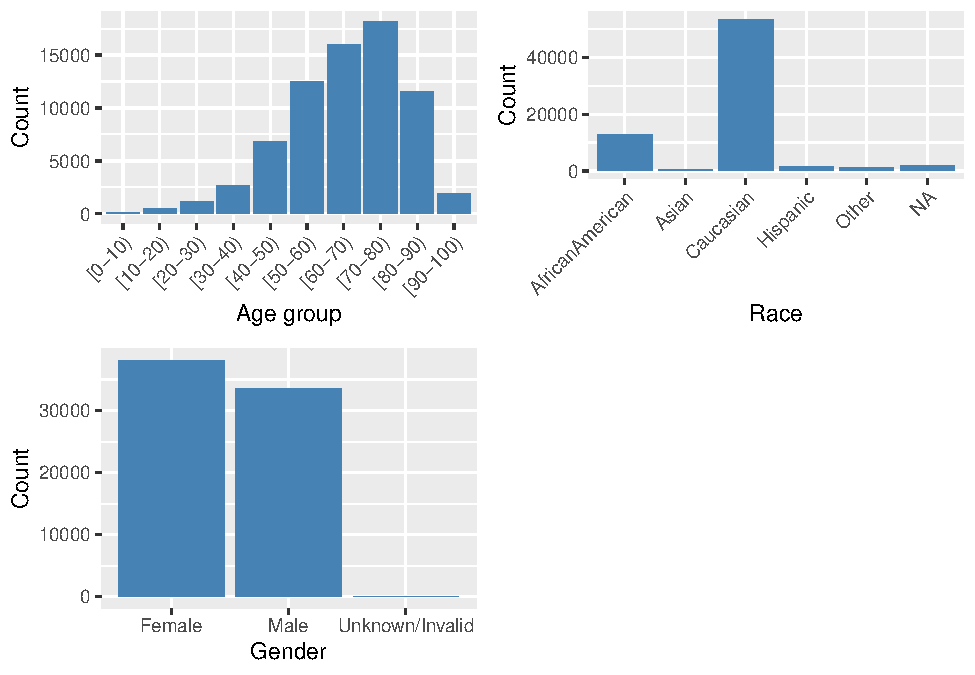
\includegraphics{exploratory_analysis_files/figure-latex/unnamed-chunk-11-1.pdf}

\hypertarget{exploration-and-feature-engineering-of-categorical-variables}{%
\section{Exploration and feature engineering of categorical
variables}\label{exploration-and-feature-engineering-of-categorical-variables}}

\hypertarget{age-race-and-gender}{%
\subsection{Age, Race, and gender}\label{age-race-and-gender}}

\hypertarget{visualisation-of-age-race-and-gender}{%
\subsubsection{Visualisation of Age, Race, and
gender}\label{visualisation-of-age-race-and-gender}}

\begin{Shaded}
\begin{Highlighting}[]
\CommentTok{\# Data manipulations are done first using spark and collected}
\NormalTok{age\_group }\OtherTok{=}\NormalTok{ diabetic\_data }\SpecialCharTok{\%\textgreater{}\%} 
  \FunctionTok{count}\NormalTok{(age) }\SpecialCharTok{\%\textgreater{}\%}
  \FunctionTok{arrange}\NormalTok{(age) }\SpecialCharTok{\%\textgreater{}\%}
  \FunctionTok{collect}\NormalTok{()}

\NormalTok{race\_group }\OtherTok{=}\NormalTok{ diabetic\_data }\SpecialCharTok{\%\textgreater{}\%} 
  \FunctionTok{count}\NormalTok{(race) }\SpecialCharTok{\%\textgreater{}\%}
  \FunctionTok{arrange}\NormalTok{(race) }\SpecialCharTok{\%\textgreater{}\%}
  \FunctionTok{collect}\NormalTok{()}

\NormalTok{gender\_group }\OtherTok{=}\NormalTok{ diabetic\_data }\SpecialCharTok{\%\textgreater{}\%} 
  \FunctionTok{count}\NormalTok{(gender) }\SpecialCharTok{\%\textgreater{}\%}
  \FunctionTok{arrange}\NormalTok{(gender) }\SpecialCharTok{\%\textgreater{}\%}
  \FunctionTok{collect}\NormalTok{()}


\CommentTok{\#plots created with ggplot}
\NormalTok{age\_plot }\OtherTok{\textless{}{-}} 
  \FunctionTok{ggplot}\NormalTok{(}\FunctionTok{aes}\NormalTok{(}\FunctionTok{as.factor}\NormalTok{(age), n), }\AttributeTok{data =}\NormalTok{ age\_group) }\SpecialCharTok{+}
  \FunctionTok{geom\_col}\NormalTok{(}\AttributeTok{fill =} \StringTok{\textquotesingle{}SteelBlue\textquotesingle{}}\NormalTok{) }\SpecialCharTok{+}
  \FunctionTok{theme}\NormalTok{(}\AttributeTok{axis.text.x =} \FunctionTok{element\_text}\NormalTok{(}\AttributeTok{angle =} \DecValTok{45}\NormalTok{, }\AttributeTok{hjust =} \DecValTok{1}\NormalTok{)) }\SpecialCharTok{+}
  \FunctionTok{xlab}\NormalTok{(}\StringTok{\textquotesingle{}Age group\textquotesingle{}}\NormalTok{) }\SpecialCharTok{+}
  \FunctionTok{ylab}\NormalTok{(}\StringTok{\textquotesingle{}Count\textquotesingle{}}\NormalTok{)}

\NormalTok{race\_plot }\OtherTok{\textless{}{-}}
  \FunctionTok{ggplot}\NormalTok{(}\FunctionTok{aes}\NormalTok{(}\FunctionTok{as.factor}\NormalTok{(race), n), }\AttributeTok{data =}\NormalTok{ race\_group) }\SpecialCharTok{+}
  \FunctionTok{geom\_col}\NormalTok{(}\AttributeTok{fill =} \StringTok{\textquotesingle{}SteelBlue\textquotesingle{}}\NormalTok{) }\SpecialCharTok{+}
  \FunctionTok{theme}\NormalTok{(}\AttributeTok{axis.text.x =} \FunctionTok{element\_text}\NormalTok{(}\AttributeTok{angle =} \DecValTok{45}\NormalTok{, }\AttributeTok{hjust =} \DecValTok{1}\NormalTok{)) }\SpecialCharTok{+}
  \FunctionTok{xlab}\NormalTok{(}\StringTok{\textquotesingle{}Race\textquotesingle{}}\NormalTok{) }\SpecialCharTok{+}
  \FunctionTok{ylab}\NormalTok{(}\StringTok{\textquotesingle{}Count\textquotesingle{}}\NormalTok{)}

\NormalTok{gender\_plot }\OtherTok{\textless{}{-}}
  \FunctionTok{ggplot}\NormalTok{(}\FunctionTok{aes}\NormalTok{(}\FunctionTok{as.factor}\NormalTok{(gender), n), }\AttributeTok{data =}\NormalTok{ gender\_group) }\SpecialCharTok{+}
  \FunctionTok{geom\_col}\NormalTok{(}\AttributeTok{fill =} \StringTok{\textquotesingle{}SteelBlue\textquotesingle{}}\NormalTok{) }\SpecialCharTok{+}
  \FunctionTok{xlab}\NormalTok{(}\StringTok{\textquotesingle{}Gender\textquotesingle{}}\NormalTok{) }\SpecialCharTok{+}
  \FunctionTok{ylab}\NormalTok{(}\StringTok{\textquotesingle{}Count\textquotesingle{}}\NormalTok{)}


\FunctionTok{plot\_grid}\NormalTok{(age\_plot, race\_plot, gender\_plot)}
\end{Highlighting}
\end{Shaded}

\includegraphics{exploratory_analysis_files/figure-latex/unnamed-chunk-12-1.pdf}

\hypertarget{feature-engineering-of-age}{%
\subsubsection{Feature engineering of
`Age'}\label{feature-engineering-of-age}}

Age is converted to an ordinal scale, using the central age from each
category. i.e.~patients classed as age `{[}10-20)' are given the value.

\begin{Shaded}
\begin{Highlighting}[]
\NormalTok{diabetic\_data }\OtherTok{\textless{}{-}}\NormalTok{ diabetic\_data }\SpecialCharTok{\%\textgreater{}\%}
  \FunctionTok{mutate}\NormalTok{(}
    \AttributeTok{age\_contin =} \FunctionTok{case\_when}\NormalTok{(}
\NormalTok{      age }\SpecialCharTok{==} \StringTok{\textquotesingle{}[0{-}10)\textquotesingle{}}    \SpecialCharTok{\textasciitilde{}} \DecValTok{5}\NormalTok{,}
\NormalTok{      age }\SpecialCharTok{==} \StringTok{\textquotesingle{}[10{-}20)\textquotesingle{}}   \SpecialCharTok{\textasciitilde{}} \DecValTok{15}\NormalTok{,}
\NormalTok{      age }\SpecialCharTok{==} \StringTok{\textquotesingle{}[20{-}30)\textquotesingle{}}   \SpecialCharTok{\textasciitilde{}} \DecValTok{25}\NormalTok{,}
\NormalTok{      age }\SpecialCharTok{==} \StringTok{\textquotesingle{}[30{-}40)\textquotesingle{}}   \SpecialCharTok{\textasciitilde{}} \DecValTok{35}\NormalTok{,}
\NormalTok{      age }\SpecialCharTok{==} \StringTok{\textquotesingle{}[40{-}50)\textquotesingle{}}   \SpecialCharTok{\textasciitilde{}} \DecValTok{45}\NormalTok{,}
\NormalTok{      age }\SpecialCharTok{==} \StringTok{\textquotesingle{}[50{-}60)\textquotesingle{}}   \SpecialCharTok{\textasciitilde{}} \DecValTok{55}\NormalTok{,}
\NormalTok{      age }\SpecialCharTok{==} \StringTok{\textquotesingle{}[60{-}70)\textquotesingle{}}   \SpecialCharTok{\textasciitilde{}} \DecValTok{65}\NormalTok{,}
\NormalTok{      age }\SpecialCharTok{==} \StringTok{\textquotesingle{}[70{-}80)\textquotesingle{}}   \SpecialCharTok{\textasciitilde{}} \DecValTok{75}\NormalTok{,}
\NormalTok{      age }\SpecialCharTok{==} \StringTok{\textquotesingle{}[80{-}90)\textquotesingle{}}   \SpecialCharTok{\textasciitilde{}} \DecValTok{85}\NormalTok{,}
\NormalTok{      age }\SpecialCharTok{==} \StringTok{\textquotesingle{}[90{-}100)\textquotesingle{}}  \SpecialCharTok{\textasciitilde{}} \DecValTok{95}
\NormalTok{    ))}
\end{Highlighting}
\end{Shaded}

\hypertarget{feature-engineering-of-race}{%
\subsubsection{Feature engineering of
`Race'}\label{feature-engineering-of-race}}

Race is one hot encoded

\begin{Shaded}
\begin{Highlighting}[]
\NormalTok{diabetic\_data }\OtherTok{\textless{}{-}}\NormalTok{ diabetic\_data }\SpecialCharTok{\%\textgreater{}\%}
  \FunctionTok{mutate}\NormalTok{(}
    \AttributeTok{unknown\_race =} \FunctionTok{ifelse}\NormalTok{(}\FunctionTok{is.na}\NormalTok{(race), }\DecValTok{1}\NormalTok{,}\DecValTok{0}\NormalTok{),}
    \AttributeTok{asian =} \FunctionTok{ifelse}\NormalTok{(race }\SpecialCharTok{==} \StringTok{\textquotesingle{}Asian\textquotesingle{}} \SpecialCharTok{\&} \SpecialCharTok{!}\FunctionTok{is.na}\NormalTok{(race), }\DecValTok{1}\NormalTok{,}\DecValTok{0}\NormalTok{),}
    \AttributeTok{african\_american =} \FunctionTok{ifelse}\NormalTok{(race }\SpecialCharTok{==} \StringTok{\textquotesingle{}AfricanAmerican\textquotesingle{}} \SpecialCharTok{\&} \SpecialCharTok{!}\FunctionTok{is.na}\NormalTok{(race), }\DecValTok{1}\NormalTok{,}\DecValTok{0}\NormalTok{),}
    \AttributeTok{caucasian =} \FunctionTok{ifelse}\NormalTok{(race }\SpecialCharTok{==} \StringTok{\textquotesingle{}Caucasian\textquotesingle{}} \SpecialCharTok{\&} \SpecialCharTok{!}\FunctionTok{is.na}\NormalTok{(race), }\DecValTok{1}\NormalTok{,}\DecValTok{0}\NormalTok{),}
    \AttributeTok{hispanic =} \FunctionTok{ifelse}\NormalTok{(race }\SpecialCharTok{==} \StringTok{\textquotesingle{}Hispanic\textquotesingle{}} \SpecialCharTok{\&} \SpecialCharTok{!}\FunctionTok{is.na}\NormalTok{(race), }\DecValTok{1}\NormalTok{,}\DecValTok{0}\NormalTok{),}
    \AttributeTok{other =} \FunctionTok{ifelse}\NormalTok{(race }\SpecialCharTok{==} \StringTok{\textquotesingle{}Other\textquotesingle{}} \SpecialCharTok{\&} \SpecialCharTok{!}\FunctionTok{is.na}\NormalTok{(race), }\DecValTok{1}\NormalTok{,}\DecValTok{0}\NormalTok{),}
\NormalTok{  )}
\end{Highlighting}
\end{Shaded}

\hypertarget{feature-engineering-of-gender}{%
\subsubsection{Feature engineering of
`Gender'}\label{feature-engineering-of-gender}}

Gender is on hot encoded

\begin{Shaded}
\begin{Highlighting}[]
\NormalTok{diabetic\_data }\OtherTok{\textless{}{-}}\NormalTok{ diabetic\_data }\SpecialCharTok{\%\textgreater{}\%}
  \FunctionTok{mutate}\NormalTok{(}
    \AttributeTok{female =} \FunctionTok{ifelse}\NormalTok{(gender }\SpecialCharTok{==} \StringTok{\textquotesingle{}Female\textquotesingle{}}\NormalTok{, }\DecValTok{1}\NormalTok{,}\DecValTok{0}\NormalTok{),}
    \AttributeTok{gender\_unknown\_invalid =} \FunctionTok{ifelse}\NormalTok{(gender }\SpecialCharTok{==} \StringTok{\textquotesingle{}Unknown/Invalid\textquotesingle{}}\NormalTok{, }\DecValTok{1}\NormalTok{,}\DecValTok{0}\NormalTok{),}
    \AttributeTok{male =} \FunctionTok{ifelse}\NormalTok{(gender }\SpecialCharTok{==} \StringTok{\textquotesingle{}Male\textquotesingle{}}\NormalTok{, }\DecValTok{1}\NormalTok{,}\DecValTok{0}\NormalTok{)}
\NormalTok{  )}
\end{Highlighting}
\end{Shaded}

\hypertarget{readmissions}{%
\subsection{Readmissions}\label{readmissions}}

View the breakdown of readmissions

\begin{Shaded}
\begin{Highlighting}[]
\NormalTok{diabetic\_data }\SpecialCharTok{\%\textgreater{}\%} 
  \FunctionTok{count}\NormalTok{(readmitted) }\SpecialCharTok{\%\textgreater{}\%}
\FunctionTok{kable}\NormalTok{(}
  \AttributeTok{caption =} \StringTok{"Summary of readmitted feature"}\NormalTok{,}
  \AttributeTok{digits =} \DecValTok{3}\NormalTok{,}
  \AttributeTok{format.args =} \FunctionTok{list}\NormalTok{(}
    \AttributeTok{big.mark =} \StringTok{","}\NormalTok{,}
    \AttributeTok{scientific =} \ConstantTok{FALSE}\NormalTok{)}
\NormalTok{  ) }\SpecialCharTok{\%\textgreater{}\%}
  \FunctionTok{kable\_styling}\NormalTok{(}\AttributeTok{latex\_options =} \StringTok{"scale\_down"}\NormalTok{) }\SpecialCharTok{\%\textgreater{}\%}
  \FunctionTok{kable\_styling}\NormalTok{(}\AttributeTok{latex\_options =} \StringTok{"HOLD\_position"}\NormalTok{)}
\end{Highlighting}
\end{Shaded}

\begin{table}[H]

\caption{\label{tab:unnamed-chunk-16}Summary of readmitted feature}
\centering
\resizebox{\linewidth}{!}{
\begin{tabular}[t]{l|r}
\hline
readmitted & n\\
\hline
<30 & 6,293\\
\hline
NO & 42,985\\
\hline
>30 & 22,240\\
\hline
\end{tabular}}
\end{table}

\hypertarget{feature-engineering-of-readmission-data}{%
\subsubsection{Feature engineering of readmission
data}\label{feature-engineering-of-readmission-data}}

A variable (\texttt{early\_readmission}) is created that classifies
those readmitted within 30 days and those not, as this is the specific
question posed by the challenge.

\begin{Shaded}
\begin{Highlighting}[]
\DocumentationTok{\#\# create a new column with readmission \textless{}30}
\NormalTok{diabetic\_data }\OtherTok{=} \FunctionTok{mutate}\NormalTok{(diabetic\_data, }\AttributeTok{early\_readmission =} \FunctionTok{ifelse}\NormalTok{(readmitted }\SpecialCharTok{==}
    \StringTok{"\textless{}30"}\NormalTok{, }\DecValTok{1}\NormalTok{, }\DecValTok{0}\NormalTok{))}

\NormalTok{diabetic\_data }\SpecialCharTok{\%\textgreater{}\%}
    \FunctionTok{group\_by}\NormalTok{(early\_readmission) }\SpecialCharTok{\%\textgreater{}\%}
    \FunctionTok{tally}\NormalTok{() }\SpecialCharTok{\%\textgreater{}\%}
    \FunctionTok{kable}\NormalTok{(}\AttributeTok{caption =} \StringTok{"Summary of early\_readmission feature"}\NormalTok{,}
        \AttributeTok{digits =} \DecValTok{3}\NormalTok{, }\AttributeTok{format.args =} \FunctionTok{list}\NormalTok{(}\AttributeTok{big.mark =} \StringTok{","}\NormalTok{,}
            \AttributeTok{scientific =} \ConstantTok{FALSE}\NormalTok{)) }\SpecialCharTok{\%\textgreater{}\%}
    \FunctionTok{kable\_styling}\NormalTok{(}\AttributeTok{latex\_options =} \StringTok{"scale\_down"}\NormalTok{) }\SpecialCharTok{\%\textgreater{}\%}
    \FunctionTok{kable\_styling}\NormalTok{(}\AttributeTok{latex\_options =} \StringTok{"HOLD\_position"}\NormalTok{)}
\end{Highlighting}
\end{Shaded}

\begin{table}[H]

\caption{\label{tab:unnamed-chunk-17}Summary of early_readmission feature}
\centering
\resizebox{\linewidth}{!}{
\begin{tabular}[t]{r|r}
\hline
early\_readmission & n\\
\hline
1 & 6,293\\
\hline
0 & 65,225\\
\hline
\end{tabular}}
\end{table}

\hypertarget{diagnoses}{%
\subsection{Diagnoses}\label{diagnoses}}

With regard to the diagnosis variables (\texttt{diag\_1},
\texttt{diag\_2}, and \texttt{diag\_3}) initial exploration determines
the exact number of different diagnosis categories.

\begin{Shaded}
\begin{Highlighting}[]
\CommentTok{\# count of the number of unique primary Dx (698)}
\NormalTok{n\_primary\_dx }\OtherTok{\textless{}{-}}\NormalTok{ diabetic\_data }\SpecialCharTok{\%\textgreater{}\%}
    \FunctionTok{summarise}\NormalTok{(}\AttributeTok{count =} \FunctionTok{n\_distinct}\NormalTok{(diag\_1)) }\SpecialCharTok{\%\textgreater{}\%}
    \FunctionTok{pull}\NormalTok{()}

\CommentTok{\# count of the number of unique secondary Dx}
\CommentTok{\# (749)}
\NormalTok{n\_secondary\_dx }\OtherTok{\textless{}{-}}\NormalTok{ diabetic\_data }\SpecialCharTok{\%\textgreater{}\%}
    \FunctionTok{summarise}\NormalTok{(}\AttributeTok{count =} \FunctionTok{n\_distinct}\NormalTok{(diag\_2)) }\SpecialCharTok{\%\textgreater{}\%}
    \FunctionTok{pull}\NormalTok{()}

\CommentTok{\# count of the number of unique tertiary Dx (759)}
\NormalTok{n\_tertiary\_dx }\OtherTok{\textless{}{-}}\NormalTok{ diabetic\_data }\SpecialCharTok{\%\textgreater{}\%}
    \FunctionTok{summarise}\NormalTok{(}\AttributeTok{count =} \FunctionTok{n\_distinct}\NormalTok{(diag\_3)) }\SpecialCharTok{\%\textgreater{}\%}
    \FunctionTok{pull}\NormalTok{()}

\NormalTok{diagnosis\_n }\OtherTok{\textless{}{-}} \FunctionTok{data.frame}\NormalTok{(}\AttributeTok{n =} \FunctionTok{c}\NormalTok{(n\_primary\_dx, n\_secondary\_dx,}
\NormalTok{    n\_tertiary\_dx))}
\FunctionTok{row.names}\NormalTok{(diagnosis\_n) }\OtherTok{\textless{}{-}} \FunctionTok{c}\NormalTok{(}\StringTok{"Primary Dx"}\NormalTok{, }\StringTok{"Secondary Dx:"}\NormalTok{,}
    \StringTok{"Tertiary Dx"}\NormalTok{)}
\FunctionTok{kable}\NormalTok{(diagnosis\_n, }\AttributeTok{caption =} \StringTok{"Total number of different diagnosis categories"}\NormalTok{,}
    \AttributeTok{digits =} \DecValTok{3}\NormalTok{, }\AttributeTok{format.args =} \FunctionTok{list}\NormalTok{(}\AttributeTok{big.mark =} \StringTok{","}\NormalTok{,}
        \AttributeTok{scientific =} \ConstantTok{FALSE}\NormalTok{)) }\SpecialCharTok{\%\textgreater{}\%}
    \FunctionTok{kable\_styling}\NormalTok{(}\AttributeTok{latex\_options =} \StringTok{"HOLD\_position"}\NormalTok{)}
\end{Highlighting}
\end{Shaded}

\begin{table}[H]

\caption{\label{tab:unnamed-chunk-18}Total number of different diagnosis categories}
\centering
\begin{tabular}[t]{l|r}
\hline
  & n\\
\hline
Primary Dx & 697\\
\hline
Secondary Dx: & 726\\
\hline
Tertiary Dx & 759\\
\hline
\end{tabular}
\end{table}

\hypertarget{feature-engineering-of-diagnosis-variables}{%
\subsubsection{Feature engineering of Diagnosis
variables}\label{feature-engineering-of-diagnosis-variables}}

As illustrated above there are 698 unique primary diagnoses, 749 unique
secondary diagnoses, and 759 tertiary diagnoses. Maintaining categorical
variables with such high levels will be computationally expensive,
diagnoses will be consolidated into more manageable levels. This is
performed below using the ICD-9 code. Diagnoses have been consolidated
according to the ICD-9 chapters, with each chapter essentially
representing a different bodily system. A seperate category for diabetes
has also been created. It should be noted that this still results in 19
categories.

\hypertarget{consolidation-of-diag_1-diag_2-and-diag_3-variables}{%
\paragraph{\texorpdfstring{Consolidation of \texttt{diag\_1},
\texttt{diag\_2}, and \texttt{diag\_3}
variables}{Consolidation of diag\_1, diag\_2, and diag\_3 variables}}\label{consolidation-of-diag_1-diag_2-and-diag_3-variables}}

\begin{Shaded}
\begin{Highlighting}[]
\CommentTok{\#consolidate according to ICD9 code}
\NormalTok{diabetic\_data }\OtherTok{\textless{}{-}}\NormalTok{ diabetic\_data }\SpecialCharTok{\%\textgreater{}\%}
  \FunctionTok{mutate}\NormalTok{(}
    \AttributeTok{diag\_1\_cat =} \FunctionTok{case\_when}\NormalTok{(}
      \FunctionTok{rlike}\NormalTok{(diag\_1, }\StringTok{"250"}\NormalTok{) }\SpecialCharTok{\textasciitilde{}} \StringTok{\textquotesingle{}diabetes\textquotesingle{}}\NormalTok{, }\CommentTok{\#case\_when works in order therefore \textquotesingle{}diabetes\textquotesingle{} will be classed before \textquotesingle{}endo\_metabolic\_immunity\textquotesingle{}}
\NormalTok{      diag\_1 }\SpecialCharTok{\textgreater{}=} \DecValTok{000} \SpecialCharTok{\&}\NormalTok{ diag\_1 }\SpecialCharTok{\textless{}} \DecValTok{140} \SpecialCharTok{\textasciitilde{}} \StringTok{\textquotesingle{}infection\textquotesingle{}}\NormalTok{,}
\NormalTok{      diag\_1 }\SpecialCharTok{\textgreater{}=} \DecValTok{140} \SpecialCharTok{\&}\NormalTok{ diag\_1 }\SpecialCharTok{\textless{}} \DecValTok{240} \SpecialCharTok{\textasciitilde{}} \StringTok{\textquotesingle{}neoplasms\textquotesingle{}}\NormalTok{,}
\NormalTok{      diag\_1 }\SpecialCharTok{\textgreater{}=} \DecValTok{240} \SpecialCharTok{\&}\NormalTok{ diag\_1 }\SpecialCharTok{\textless{}} \DecValTok{280} \SpecialCharTok{\textasciitilde{}} \StringTok{\textquotesingle{}endo\_metabolic\_immunity\textquotesingle{}}\NormalTok{,}
\NormalTok{      diag\_1 }\SpecialCharTok{\textgreater{}=} \DecValTok{280} \SpecialCharTok{\&}\NormalTok{ diag\_1 }\SpecialCharTok{\textless{}} \DecValTok{290} \SpecialCharTok{\textasciitilde{}} \StringTok{\textquotesingle{}haematology\textquotesingle{}}\NormalTok{,}
\NormalTok{      diag\_1 }\SpecialCharTok{\textgreater{}=} \DecValTok{290} \SpecialCharTok{\&}\NormalTok{ diag\_1 }\SpecialCharTok{\textless{}} \DecValTok{320} \SpecialCharTok{\textasciitilde{}} \StringTok{\textquotesingle{}mental\textquotesingle{}}\NormalTok{,}
\NormalTok{      diag\_1 }\SpecialCharTok{\textgreater{}=} \DecValTok{320} \SpecialCharTok{\&}\NormalTok{ diag\_1 }\SpecialCharTok{\textless{}} \DecValTok{390} \SpecialCharTok{\textasciitilde{}} \StringTok{\textquotesingle{}neurology\textquotesingle{}}\NormalTok{,}
\NormalTok{      diag\_1 }\SpecialCharTok{\textgreater{}=} \DecValTok{390} \SpecialCharTok{\&}\NormalTok{ diag\_1 }\SpecialCharTok{\textless{}} \DecValTok{460} \SpecialCharTok{\textasciitilde{}} \StringTok{\textquotesingle{}circulatory\textquotesingle{}}\NormalTok{,}
\NormalTok{      diag\_1 }\SpecialCharTok{\textgreater{}=} \DecValTok{460} \SpecialCharTok{\&}\NormalTok{ diag\_1 }\SpecialCharTok{\textless{}} \DecValTok{520} \SpecialCharTok{\textasciitilde{}} \StringTok{\textquotesingle{}respiratory\textquotesingle{}}\NormalTok{,}
\NormalTok{      diag\_1 }\SpecialCharTok{\textgreater{}=} \DecValTok{520} \SpecialCharTok{\&}\NormalTok{ diag\_1 }\SpecialCharTok{\textless{}} \DecValTok{580} \SpecialCharTok{\textasciitilde{}} \StringTok{\textquotesingle{}digestive\textquotesingle{}}\NormalTok{,}
\NormalTok{      diag\_1 }\SpecialCharTok{\textgreater{}=} \DecValTok{580} \SpecialCharTok{\&}\NormalTok{ diag\_1 }\SpecialCharTok{\textless{}} \DecValTok{630} \SpecialCharTok{\textasciitilde{}} \StringTok{\textquotesingle{}genitourinary\textquotesingle{}}\NormalTok{,}
\NormalTok{      diag\_1 }\SpecialCharTok{\textgreater{}=} \DecValTok{630} \SpecialCharTok{\&}\NormalTok{ diag\_1 }\SpecialCharTok{\textless{}} \DecValTok{680} \SpecialCharTok{\textasciitilde{}} \StringTok{\textquotesingle{}preg\_birth\_puerperium\textquotesingle{}}\NormalTok{,}
\NormalTok{      diag\_1 }\SpecialCharTok{\textgreater{}=} \DecValTok{680} \SpecialCharTok{\&}\NormalTok{ diag\_1 }\SpecialCharTok{\textless{}} \DecValTok{710} \SpecialCharTok{\textasciitilde{}} \StringTok{\textquotesingle{}dermatology\textquotesingle{}}\NormalTok{,}
\NormalTok{      diag\_1 }\SpecialCharTok{\textgreater{}=} \DecValTok{710} \SpecialCharTok{\&}\NormalTok{ diag\_1 }\SpecialCharTok{\textless{}} \DecValTok{740} \SpecialCharTok{\textasciitilde{}} \StringTok{\textquotesingle{}musculoskeletal\textquotesingle{}}\NormalTok{,}
\NormalTok{      diag\_1 }\SpecialCharTok{\textgreater{}=} \DecValTok{740} \SpecialCharTok{\&}\NormalTok{ diag\_1 }\SpecialCharTok{\textless{}} \DecValTok{760} \SpecialCharTok{\textasciitilde{}} \StringTok{\textquotesingle{}congenital\textquotesingle{}}\NormalTok{,}
\NormalTok{      diag\_1 }\SpecialCharTok{\textgreater{}=} \DecValTok{760} \SpecialCharTok{\&}\NormalTok{ diag\_1 }\SpecialCharTok{\textless{}} \DecValTok{780} \SpecialCharTok{\textasciitilde{}} \StringTok{\textquotesingle{}perinatal\textquotesingle{}}\NormalTok{,}
\NormalTok{      diag\_1 }\SpecialCharTok{\textgreater{}=} \DecValTok{780} \SpecialCharTok{\&}\NormalTok{ diag\_1 }\SpecialCharTok{\textless{}} \DecValTok{800} \SpecialCharTok{\textasciitilde{}} \StringTok{\textquotesingle{}ill\_defined\textquotesingle{}}\NormalTok{,}
\NormalTok{      diag\_1 }\SpecialCharTok{\textgreater{}=} \DecValTok{800} \SpecialCharTok{\&}\NormalTok{ diag\_1 }\SpecialCharTok{\textless{}} \DecValTok{1000} \SpecialCharTok{\textasciitilde{}} \StringTok{\textquotesingle{}injury\_poisoning\textquotesingle{}}\NormalTok{,}
      \FunctionTok{rlike}\NormalTok{(diag\_1, }\StringTok{"V"}\NormalTok{) }\SpecialCharTok{|} \FunctionTok{rlike}\NormalTok{(diag\_1, }\StringTok{"E"}\NormalTok{) }\SpecialCharTok{\textasciitilde{}} \StringTok{\textquotesingle{}supplementary\textquotesingle{}}\NormalTok{,}
      \FunctionTok{is.na}\NormalTok{(diag\_1) }\SpecialCharTok{\textasciitilde{}} \StringTok{\textquotesingle{}unknown\_diag\_1\textquotesingle{}}\NormalTok{, }\CommentTok{\#NA variables do not get special treatment}
      \ConstantTok{TRUE} \SpecialCharTok{\textasciitilde{}}\NormalTok{ diag\_1),}
    \AttributeTok{diag\_2\_cat =} \FunctionTok{case\_when}\NormalTok{(}
      \FunctionTok{rlike}\NormalTok{(diag\_2, }\StringTok{"250"}\NormalTok{) }\SpecialCharTok{\textasciitilde{}} \StringTok{\textquotesingle{}diabetes\textquotesingle{}}\NormalTok{, }\CommentTok{\#case\_when work in order}
\NormalTok{      diag\_2 }\SpecialCharTok{\textgreater{}=} \DecValTok{000} \SpecialCharTok{\&}\NormalTok{ diag\_2 }\SpecialCharTok{\textless{}} \DecValTok{140} \SpecialCharTok{\textasciitilde{}} \StringTok{\textquotesingle{}infection\textquotesingle{}}\NormalTok{,}
\NormalTok{      diag\_2 }\SpecialCharTok{\textgreater{}=} \DecValTok{140} \SpecialCharTok{\&}\NormalTok{ diag\_2 }\SpecialCharTok{\textless{}} \DecValTok{240} \SpecialCharTok{\textasciitilde{}} \StringTok{\textquotesingle{}neoplasms\textquotesingle{}}\NormalTok{,}
\NormalTok{      diag\_2 }\SpecialCharTok{\textgreater{}=} \DecValTok{240} \SpecialCharTok{\&}\NormalTok{ diag\_2 }\SpecialCharTok{\textless{}} \DecValTok{280} \SpecialCharTok{\textasciitilde{}} \StringTok{\textquotesingle{}endo\_metabolic\_immunity\textquotesingle{}}\NormalTok{,}
\NormalTok{      diag\_2 }\SpecialCharTok{\textgreater{}=} \DecValTok{280} \SpecialCharTok{\&}\NormalTok{ diag\_2 }\SpecialCharTok{\textless{}} \DecValTok{290} \SpecialCharTok{\textasciitilde{}} \StringTok{\textquotesingle{}haematology\textquotesingle{}}\NormalTok{,}
\NormalTok{      diag\_2 }\SpecialCharTok{\textgreater{}=} \DecValTok{290} \SpecialCharTok{\&}\NormalTok{ diag\_2 }\SpecialCharTok{\textless{}} \DecValTok{320} \SpecialCharTok{\textasciitilde{}} \StringTok{\textquotesingle{}mental\textquotesingle{}}\NormalTok{,}
\NormalTok{      diag\_2 }\SpecialCharTok{\textgreater{}=} \DecValTok{320} \SpecialCharTok{\&}\NormalTok{ diag\_2 }\SpecialCharTok{\textless{}} \DecValTok{390} \SpecialCharTok{\textasciitilde{}} \StringTok{\textquotesingle{}neurology\textquotesingle{}}\NormalTok{,}
\NormalTok{      diag\_2 }\SpecialCharTok{\textgreater{}=} \DecValTok{390} \SpecialCharTok{\&}\NormalTok{ diag\_2 }\SpecialCharTok{\textless{}} \DecValTok{460} \SpecialCharTok{\textasciitilde{}} \StringTok{\textquotesingle{}circulatory\textquotesingle{}}\NormalTok{,}
\NormalTok{      diag\_2 }\SpecialCharTok{\textgreater{}=} \DecValTok{460} \SpecialCharTok{\&}\NormalTok{ diag\_2 }\SpecialCharTok{\textless{}} \DecValTok{520} \SpecialCharTok{\textasciitilde{}} \StringTok{\textquotesingle{}respiratory\textquotesingle{}}\NormalTok{,}
\NormalTok{      diag\_2 }\SpecialCharTok{\textgreater{}=} \DecValTok{520} \SpecialCharTok{\&}\NormalTok{ diag\_2 }\SpecialCharTok{\textless{}} \DecValTok{580} \SpecialCharTok{\textasciitilde{}} \StringTok{\textquotesingle{}digestive\textquotesingle{}}\NormalTok{,}
\NormalTok{      diag\_2 }\SpecialCharTok{\textgreater{}=} \DecValTok{580} \SpecialCharTok{\&}\NormalTok{ diag\_2 }\SpecialCharTok{\textless{}} \DecValTok{630} \SpecialCharTok{\textasciitilde{}} \StringTok{\textquotesingle{}genitourinary\textquotesingle{}}\NormalTok{,}
\NormalTok{      diag\_2 }\SpecialCharTok{\textgreater{}=} \DecValTok{630} \SpecialCharTok{\&}\NormalTok{ diag\_2 }\SpecialCharTok{\textless{}} \DecValTok{680} \SpecialCharTok{\textasciitilde{}} \StringTok{\textquotesingle{}preg\_birth\_puerperium\textquotesingle{}}\NormalTok{,}
\NormalTok{      diag\_2 }\SpecialCharTok{\textgreater{}=} \DecValTok{680} \SpecialCharTok{\&}\NormalTok{ diag\_2 }\SpecialCharTok{\textless{}} \DecValTok{710} \SpecialCharTok{\textasciitilde{}} \StringTok{\textquotesingle{}dermatology\textquotesingle{}}\NormalTok{,}
\NormalTok{      diag\_2 }\SpecialCharTok{\textgreater{}=} \DecValTok{710} \SpecialCharTok{\&}\NormalTok{ diag\_2 }\SpecialCharTok{\textless{}} \DecValTok{740} \SpecialCharTok{\textasciitilde{}} \StringTok{\textquotesingle{}musculoskeletal\textquotesingle{}}\NormalTok{,}
\NormalTok{      diag\_2 }\SpecialCharTok{\textgreater{}=} \DecValTok{740} \SpecialCharTok{\&}\NormalTok{ diag\_2 }\SpecialCharTok{\textless{}} \DecValTok{760} \SpecialCharTok{\textasciitilde{}} \StringTok{\textquotesingle{}congenital\textquotesingle{}}\NormalTok{,}
\NormalTok{      diag\_2 }\SpecialCharTok{\textgreater{}=} \DecValTok{760} \SpecialCharTok{\&}\NormalTok{ diag\_2 }\SpecialCharTok{\textless{}} \DecValTok{780} \SpecialCharTok{\textasciitilde{}} \StringTok{\textquotesingle{}perinatal\textquotesingle{}}\NormalTok{,}
\NormalTok{      diag\_2 }\SpecialCharTok{\textgreater{}=} \DecValTok{780} \SpecialCharTok{\&}\NormalTok{ diag\_2 }\SpecialCharTok{\textless{}} \DecValTok{800} \SpecialCharTok{\textasciitilde{}} \StringTok{\textquotesingle{}ill\_defined\textquotesingle{}}\NormalTok{,}
\NormalTok{      diag\_2 }\SpecialCharTok{\textgreater{}=} \DecValTok{800} \SpecialCharTok{\&}\NormalTok{ diag\_2 }\SpecialCharTok{\textless{}} \DecValTok{1000} \SpecialCharTok{\textasciitilde{}} \StringTok{\textquotesingle{}injury\_poisoning\textquotesingle{}}\NormalTok{,}
      \FunctionTok{rlike}\NormalTok{(diag\_2, }\StringTok{"V"}\NormalTok{) }\SpecialCharTok{|} \FunctionTok{rlike}\NormalTok{(diag\_2, }\StringTok{"E"}\NormalTok{) }\SpecialCharTok{\textasciitilde{}} \StringTok{\textquotesingle{}supplementary\textquotesingle{}}\NormalTok{,}
      \FunctionTok{is.na}\NormalTok{(diag\_2) }\SpecialCharTok{\textasciitilde{}} \StringTok{\textquotesingle{}unknown\_diag\_2\textquotesingle{}}\NormalTok{, }\CommentTok{\#NA variable do not get special treatment}
      \ConstantTok{TRUE} \SpecialCharTok{\textasciitilde{}}\NormalTok{ diag\_2),}
    \AttributeTok{diag\_3\_cat =} \FunctionTok{case\_when}\NormalTok{(}
      \FunctionTok{rlike}\NormalTok{(diag\_3, }\StringTok{"250"}\NormalTok{) }\SpecialCharTok{\textasciitilde{}} \StringTok{\textquotesingle{}diabetes\textquotesingle{}}\NormalTok{, }\CommentTok{\#case\_when work in order}
\NormalTok{      diag\_3 }\SpecialCharTok{\textgreater{}=} \DecValTok{000} \SpecialCharTok{\&}\NormalTok{ diag\_3 }\SpecialCharTok{\textless{}} \DecValTok{140} \SpecialCharTok{\textasciitilde{}} \StringTok{\textquotesingle{}infection\textquotesingle{}}\NormalTok{,}
\NormalTok{      diag\_3 }\SpecialCharTok{\textgreater{}=} \DecValTok{140} \SpecialCharTok{\&}\NormalTok{ diag\_3 }\SpecialCharTok{\textless{}} \DecValTok{240} \SpecialCharTok{\textasciitilde{}} \StringTok{\textquotesingle{}neoplasms\textquotesingle{}}\NormalTok{,}
\NormalTok{      diag\_3 }\SpecialCharTok{\textgreater{}=} \DecValTok{240} \SpecialCharTok{\&}\NormalTok{ diag\_3 }\SpecialCharTok{\textless{}} \DecValTok{280} \SpecialCharTok{\textasciitilde{}} \StringTok{\textquotesingle{}endo\_metabolic\_immunity\textquotesingle{}}\NormalTok{,}
\NormalTok{      diag\_3 }\SpecialCharTok{\textgreater{}=} \DecValTok{280} \SpecialCharTok{\&}\NormalTok{ diag\_3 }\SpecialCharTok{\textless{}} \DecValTok{290} \SpecialCharTok{\textasciitilde{}} \StringTok{\textquotesingle{}haematology\textquotesingle{}}\NormalTok{,}
\NormalTok{      diag\_3 }\SpecialCharTok{\textgreater{}=} \DecValTok{290} \SpecialCharTok{\&}\NormalTok{ diag\_3 }\SpecialCharTok{\textless{}} \DecValTok{320} \SpecialCharTok{\textasciitilde{}} \StringTok{\textquotesingle{}mental\textquotesingle{}}\NormalTok{,}
\NormalTok{      diag\_3 }\SpecialCharTok{\textgreater{}=} \DecValTok{320} \SpecialCharTok{\&}\NormalTok{ diag\_3 }\SpecialCharTok{\textless{}} \DecValTok{390} \SpecialCharTok{\textasciitilde{}} \StringTok{\textquotesingle{}neurology\textquotesingle{}}\NormalTok{,}
\NormalTok{      diag\_3 }\SpecialCharTok{\textgreater{}=} \DecValTok{390} \SpecialCharTok{\&}\NormalTok{ diag\_3 }\SpecialCharTok{\textless{}} \DecValTok{460} \SpecialCharTok{\textasciitilde{}} \StringTok{\textquotesingle{}circulatory\textquotesingle{}}\NormalTok{,}
\NormalTok{      diag\_3 }\SpecialCharTok{\textgreater{}=} \DecValTok{460} \SpecialCharTok{\&}\NormalTok{ diag\_3 }\SpecialCharTok{\textless{}} \DecValTok{520} \SpecialCharTok{\textasciitilde{}} \StringTok{\textquotesingle{}respiratory\textquotesingle{}}\NormalTok{,}
\NormalTok{      diag\_3 }\SpecialCharTok{\textgreater{}=} \DecValTok{520} \SpecialCharTok{\&}\NormalTok{ diag\_3 }\SpecialCharTok{\textless{}} \DecValTok{580} \SpecialCharTok{\textasciitilde{}} \StringTok{\textquotesingle{}digestive\textquotesingle{}}\NormalTok{,}
\NormalTok{      diag\_3 }\SpecialCharTok{\textgreater{}=} \DecValTok{580} \SpecialCharTok{\&}\NormalTok{ diag\_3 }\SpecialCharTok{\textless{}} \DecValTok{630} \SpecialCharTok{\textasciitilde{}} \StringTok{\textquotesingle{}genitourinary\textquotesingle{}}\NormalTok{,}
\NormalTok{      diag\_3 }\SpecialCharTok{\textgreater{}=} \DecValTok{630} \SpecialCharTok{\&}\NormalTok{ diag\_3 }\SpecialCharTok{\textless{}} \DecValTok{680} \SpecialCharTok{\textasciitilde{}} \StringTok{\textquotesingle{}preg\_birth\_puerperium\textquotesingle{}}\NormalTok{,}
\NormalTok{      diag\_3 }\SpecialCharTok{\textgreater{}=} \DecValTok{680} \SpecialCharTok{\&}\NormalTok{ diag\_3 }\SpecialCharTok{\textless{}} \DecValTok{710} \SpecialCharTok{\textasciitilde{}} \StringTok{\textquotesingle{}dermatology\textquotesingle{}}\NormalTok{,}
\NormalTok{      diag\_3 }\SpecialCharTok{\textgreater{}=} \DecValTok{710} \SpecialCharTok{\&}\NormalTok{ diag\_3 }\SpecialCharTok{\textless{}} \DecValTok{740} \SpecialCharTok{\textasciitilde{}} \StringTok{\textquotesingle{}musculoskeletal\textquotesingle{}}\NormalTok{,}
\NormalTok{      diag\_3 }\SpecialCharTok{\textgreater{}=} \DecValTok{740} \SpecialCharTok{\&}\NormalTok{ diag\_3 }\SpecialCharTok{\textless{}} \DecValTok{760} \SpecialCharTok{\textasciitilde{}} \StringTok{\textquotesingle{}congenital\textquotesingle{}}\NormalTok{,}
\NormalTok{      diag\_3 }\SpecialCharTok{\textgreater{}=} \DecValTok{760} \SpecialCharTok{\&}\NormalTok{ diag\_3 }\SpecialCharTok{\textless{}} \DecValTok{780} \SpecialCharTok{\textasciitilde{}} \StringTok{\textquotesingle{}perinatal\textquotesingle{}}\NormalTok{,}
\NormalTok{      diag\_3 }\SpecialCharTok{\textgreater{}=} \DecValTok{780} \SpecialCharTok{\&}\NormalTok{ diag\_3 }\SpecialCharTok{\textless{}} \DecValTok{800} \SpecialCharTok{\textasciitilde{}} \StringTok{\textquotesingle{}ill\_defined\textquotesingle{}}\NormalTok{,}
\NormalTok{      diag\_3 }\SpecialCharTok{\textgreater{}=} \DecValTok{800} \SpecialCharTok{\&}\NormalTok{ diag\_3 }\SpecialCharTok{\textless{}} \DecValTok{1000} \SpecialCharTok{\textasciitilde{}} \StringTok{\textquotesingle{}injury\_poisoning\textquotesingle{}}\NormalTok{,}
      \FunctionTok{rlike}\NormalTok{(diag\_3, }\StringTok{"V"}\NormalTok{) }\SpecialCharTok{|} \FunctionTok{rlike}\NormalTok{(diag\_3, }\StringTok{"E"}\NormalTok{) }\SpecialCharTok{\textasciitilde{}} \StringTok{\textquotesingle{}supplementary\textquotesingle{}}\NormalTok{,}
      \FunctionTok{is.na}\NormalTok{(diag\_3) }\SpecialCharTok{\textasciitilde{}} \StringTok{\textquotesingle{}unknown\_diag\_3\textquotesingle{}}\NormalTok{, }\CommentTok{\#NA variable do not get special treatment}
      \ConstantTok{TRUE} \SpecialCharTok{\textasciitilde{}}\NormalTok{ diag\_3)}
\NormalTok{  )}
\end{Highlighting}
\end{Shaded}

\hypertarget{one-hot-encoding-of-diagnnsis-categories}{%
\paragraph{One hot encoding of diagnnsis
categories}\label{one-hot-encoding-of-diagnnsis-categories}}

The diagnosis categories are then one hot encoded

\begin{Shaded}
\begin{Highlighting}[]
\CommentTok{\# one\_hot\_encode diagnosis}
\NormalTok{diabetic\_data }\OtherTok{\textless{}{-}}\NormalTok{ diabetic\_data }\SpecialCharTok{\%\textgreater{}\%}
    \FunctionTok{mutate}\NormalTok{(}\AttributeTok{diag\_1\_infection =} \FunctionTok{ifelse}\NormalTok{(diag\_1\_cat }\SpecialCharTok{==}
        \StringTok{"infection"} \SpecialCharTok{\&} \SpecialCharTok{!}\FunctionTok{is.na}\NormalTok{(diag\_1\_cat), }\DecValTok{1}\NormalTok{, }\DecValTok{0}\NormalTok{), }\AttributeTok{diag\_1\_neoplasms =} \FunctionTok{ifelse}\NormalTok{(diag\_1\_cat }\SpecialCharTok{==}
        \StringTok{"neoplasms"} \SpecialCharTok{\&} \SpecialCharTok{!}\FunctionTok{is.na}\NormalTok{(diag\_1\_cat), }\DecValTok{1}\NormalTok{, }\DecValTok{0}\NormalTok{), }\AttributeTok{diag\_1\_endo\_metabolic\_immunity =} \FunctionTok{ifelse}\NormalTok{(diag\_1\_cat }\SpecialCharTok{==}
        \StringTok{"endo\_metabolic\_immunity"} \SpecialCharTok{\&} \SpecialCharTok{!}\FunctionTok{is.na}\NormalTok{(diag\_1\_cat),}
        \DecValTok{1}\NormalTok{, }\DecValTok{0}\NormalTok{), }\AttributeTok{diag\_1\_haematology =} \FunctionTok{ifelse}\NormalTok{(diag\_1\_cat }\SpecialCharTok{==}
        \StringTok{"haematology"} \SpecialCharTok{\&} \SpecialCharTok{!}\FunctionTok{is.na}\NormalTok{(diag\_1\_cat), }\DecValTok{1}\NormalTok{, }\DecValTok{0}\NormalTok{),}
        \AttributeTok{diag\_1\_mental =} \FunctionTok{ifelse}\NormalTok{(diag\_1\_cat }\SpecialCharTok{==} \StringTok{"mental"} \SpecialCharTok{\&}
            \SpecialCharTok{!}\FunctionTok{is.na}\NormalTok{(diag\_1\_cat), }\DecValTok{1}\NormalTok{, }\DecValTok{0}\NormalTok{), }\AttributeTok{diag\_1\_neurology =} \FunctionTok{ifelse}\NormalTok{(diag\_1\_cat }\SpecialCharTok{==}
            \StringTok{"neurology"} \SpecialCharTok{\&} \SpecialCharTok{!}\FunctionTok{is.na}\NormalTok{(diag\_1\_cat), }\DecValTok{1}\NormalTok{, }\DecValTok{0}\NormalTok{),}
        \AttributeTok{diag\_1\_circulatory =} \FunctionTok{ifelse}\NormalTok{(diag\_1\_cat }\SpecialCharTok{==} \StringTok{"circulatory"} \SpecialCharTok{\&}
            \SpecialCharTok{!}\FunctionTok{is.na}\NormalTok{(diag\_1\_cat), }\DecValTok{1}\NormalTok{, }\DecValTok{0}\NormalTok{), }\AttributeTok{diag\_1\_respiratory =} \FunctionTok{ifelse}\NormalTok{(diag\_1\_cat }\SpecialCharTok{==}
            \StringTok{"respiratory"} \SpecialCharTok{\&} \SpecialCharTok{!}\FunctionTok{is.na}\NormalTok{(diag\_1\_cat), }\DecValTok{1}\NormalTok{,}
            \DecValTok{0}\NormalTok{), }\AttributeTok{diag\_1\_digestive =} \FunctionTok{ifelse}\NormalTok{(diag\_1\_cat }\SpecialCharTok{==}
            \StringTok{"digestive"} \SpecialCharTok{\&} \SpecialCharTok{!}\FunctionTok{is.na}\NormalTok{(diag\_1\_cat), }\DecValTok{1}\NormalTok{, }\DecValTok{0}\NormalTok{),}
        \AttributeTok{diag\_1\_genitourinary =} \FunctionTok{ifelse}\NormalTok{(diag\_1\_cat }\SpecialCharTok{==}
            \StringTok{"genitourinary"} \SpecialCharTok{\&} \SpecialCharTok{!}\FunctionTok{is.na}\NormalTok{(diag\_1\_cat), }\DecValTok{1}\NormalTok{,}
            \DecValTok{0}\NormalTok{), }\AttributeTok{diag\_1\_preg\_birth\_puerperium =} \FunctionTok{ifelse}\NormalTok{(diag\_1\_cat }\SpecialCharTok{==}
            \StringTok{"preg\_birth\_puerperium"} \SpecialCharTok{\&} \SpecialCharTok{!}\FunctionTok{is.na}\NormalTok{(diag\_1\_cat),}
            \DecValTok{1}\NormalTok{, }\DecValTok{0}\NormalTok{), }\AttributeTok{diag\_1\_dermatology =} \FunctionTok{ifelse}\NormalTok{(diag\_1\_cat }\SpecialCharTok{==}
            \StringTok{"dermatology"} \SpecialCharTok{\&} \SpecialCharTok{!}\FunctionTok{is.na}\NormalTok{(diag\_1\_cat), }\DecValTok{1}\NormalTok{,}
            \DecValTok{0}\NormalTok{), }\AttributeTok{diag\_1\_musculoskeletal =} \FunctionTok{ifelse}\NormalTok{(diag\_1\_cat }\SpecialCharTok{==}
            \StringTok{"musculoskeletal"} \SpecialCharTok{\&} \SpecialCharTok{!}\FunctionTok{is.na}\NormalTok{(diag\_1\_cat),}
            \DecValTok{1}\NormalTok{, }\DecValTok{0}\NormalTok{), }\AttributeTok{diag\_1\_congenital =} \FunctionTok{ifelse}\NormalTok{(diag\_1\_cat }\SpecialCharTok{==}
            \StringTok{"congenital"} \SpecialCharTok{\&} \SpecialCharTok{!}\FunctionTok{is.na}\NormalTok{(diag\_1\_cat), }\DecValTok{1}\NormalTok{, }\DecValTok{0}\NormalTok{),}
        \AttributeTok{diag\_1\_perinatal =} \FunctionTok{ifelse}\NormalTok{(diag\_1\_cat }\SpecialCharTok{==} \StringTok{"perinatal"} \SpecialCharTok{\&}
            \SpecialCharTok{!}\FunctionTok{is.na}\NormalTok{(diag\_1\_cat), }\DecValTok{1}\NormalTok{, }\DecValTok{0}\NormalTok{), }\AttributeTok{diag\_1\_ill\_defined =} \FunctionTok{ifelse}\NormalTok{(diag\_1\_cat }\SpecialCharTok{==}
            \StringTok{"ill\_defined"} \SpecialCharTok{\&} \SpecialCharTok{!}\FunctionTok{is.na}\NormalTok{(diag\_1\_cat), }\DecValTok{1}\NormalTok{,}
            \DecValTok{0}\NormalTok{), }\AttributeTok{diag\_1\_injury\_poisoning =} \FunctionTok{ifelse}\NormalTok{(diag\_1\_cat }\SpecialCharTok{==}
            \StringTok{"injury\_poisoning"} \SpecialCharTok{\&} \SpecialCharTok{!}\FunctionTok{is.na}\NormalTok{(diag\_1\_cat),}
            \DecValTok{1}\NormalTok{, }\DecValTok{0}\NormalTok{), }\AttributeTok{diag\_1\_supplementary =} \FunctionTok{ifelse}\NormalTok{(diag\_1\_cat }\SpecialCharTok{==}
            \StringTok{"supplementary"} \SpecialCharTok{\&} \SpecialCharTok{!}\FunctionTok{is.na}\NormalTok{(diag\_1\_cat), }\DecValTok{1}\NormalTok{,}
            \DecValTok{0}\NormalTok{), }\AttributeTok{diag\_1\_diabetes =} \FunctionTok{ifelse}\NormalTok{(diag\_1\_cat }\SpecialCharTok{==}
            \StringTok{"diabetes"} \SpecialCharTok{\&} \SpecialCharTok{!}\FunctionTok{is.na}\NormalTok{(diag\_1\_cat), }\DecValTok{1}\NormalTok{, }\DecValTok{0}\NormalTok{),}
        \AttributeTok{diag\_1\_unknown =} \FunctionTok{ifelse}\NormalTok{(diag\_1\_cat }\SpecialCharTok{==} \StringTok{"unknown\_diag\_1"} \SpecialCharTok{\&}
            \SpecialCharTok{!}\FunctionTok{is.na}\NormalTok{(diag\_1\_cat), }\DecValTok{1}\NormalTok{, }\DecValTok{0}\NormalTok{), }\AttributeTok{diag\_2\_infection =} \FunctionTok{ifelse}\NormalTok{(diag\_2\_cat }\SpecialCharTok{==}
            \StringTok{"infection"} \SpecialCharTok{\&} \SpecialCharTok{!}\FunctionTok{is.na}\NormalTok{(diag\_2\_cat), }\DecValTok{1}\NormalTok{, }\DecValTok{0}\NormalTok{),}
        \AttributeTok{diag\_2\_neoplasms =} \FunctionTok{ifelse}\NormalTok{(diag\_2\_cat }\SpecialCharTok{==} \StringTok{"neoplasms"} \SpecialCharTok{\&}
            \SpecialCharTok{!}\FunctionTok{is.na}\NormalTok{(diag\_2\_cat), }\DecValTok{1}\NormalTok{, }\DecValTok{0}\NormalTok{), }\AttributeTok{diag\_2\_endo\_metabolic\_immunity =} \FunctionTok{ifelse}\NormalTok{(diag\_2\_cat }\SpecialCharTok{==}
            \StringTok{"endo\_metabolic\_immunity"} \SpecialCharTok{\&} \SpecialCharTok{!}\FunctionTok{is.na}\NormalTok{(diag\_2\_cat),}
            \DecValTok{1}\NormalTok{, }\DecValTok{0}\NormalTok{), }\AttributeTok{diag\_2\_haematology =} \FunctionTok{ifelse}\NormalTok{(diag\_2\_cat }\SpecialCharTok{==}
            \StringTok{"haematology"} \SpecialCharTok{\&} \SpecialCharTok{!}\FunctionTok{is.na}\NormalTok{(diag\_2\_cat), }\DecValTok{1}\NormalTok{,}
            \DecValTok{0}\NormalTok{), }\AttributeTok{diag\_2\_mental =} \FunctionTok{ifelse}\NormalTok{(diag\_2\_cat }\SpecialCharTok{==}
            \StringTok{"mental"} \SpecialCharTok{\&} \SpecialCharTok{!}\FunctionTok{is.na}\NormalTok{(diag\_2\_cat), }\DecValTok{1}\NormalTok{, }\DecValTok{0}\NormalTok{), }\AttributeTok{diag\_2\_neurology =} \FunctionTok{ifelse}\NormalTok{(diag\_2\_cat }\SpecialCharTok{==}
            \StringTok{"neurology"} \SpecialCharTok{\&} \SpecialCharTok{!}\FunctionTok{is.na}\NormalTok{(diag\_2\_cat), }\DecValTok{1}\NormalTok{, }\DecValTok{0}\NormalTok{),}
        \AttributeTok{diag\_2\_circulatory =} \FunctionTok{ifelse}\NormalTok{(diag\_2\_cat }\SpecialCharTok{==} \StringTok{"circulatory"} \SpecialCharTok{\&}
            \SpecialCharTok{!}\FunctionTok{is.na}\NormalTok{(diag\_2\_cat), }\DecValTok{1}\NormalTok{, }\DecValTok{0}\NormalTok{), }\AttributeTok{diag\_2\_respiratory =} \FunctionTok{ifelse}\NormalTok{(diag\_2\_cat }\SpecialCharTok{==}
            \StringTok{"respiratory"} \SpecialCharTok{\&} \SpecialCharTok{!}\FunctionTok{is.na}\NormalTok{(diag\_2\_cat), }\DecValTok{1}\NormalTok{,}
            \DecValTok{0}\NormalTok{), }\AttributeTok{diag\_2\_digestive =} \FunctionTok{ifelse}\NormalTok{(diag\_2\_cat }\SpecialCharTok{==}
            \StringTok{"digestive"} \SpecialCharTok{\&} \SpecialCharTok{!}\FunctionTok{is.na}\NormalTok{(diag\_2\_cat), }\DecValTok{1}\NormalTok{, }\DecValTok{0}\NormalTok{),}
        \AttributeTok{diag\_2\_genitourinary =} \FunctionTok{ifelse}\NormalTok{(diag\_2\_cat }\SpecialCharTok{==}
            \StringTok{"genitourinary"} \SpecialCharTok{\&} \SpecialCharTok{!}\FunctionTok{is.na}\NormalTok{(diag\_2\_cat), }\DecValTok{1}\NormalTok{,}
            \DecValTok{0}\NormalTok{), }\AttributeTok{diag\_2\_preg\_birth\_puerperium =} \FunctionTok{ifelse}\NormalTok{(diag\_2\_cat }\SpecialCharTok{==}
            \StringTok{"preg\_birth\_puerperium"} \SpecialCharTok{\&} \SpecialCharTok{!}\FunctionTok{is.na}\NormalTok{(diag\_2\_cat),}
            \DecValTok{1}\NormalTok{, }\DecValTok{0}\NormalTok{), }\AttributeTok{diag\_2\_dermatology =} \FunctionTok{ifelse}\NormalTok{(diag\_2\_cat }\SpecialCharTok{==}
            \StringTok{"dermatology"} \SpecialCharTok{\&} \SpecialCharTok{!}\FunctionTok{is.na}\NormalTok{(diag\_2\_cat), }\DecValTok{1}\NormalTok{,}
            \DecValTok{0}\NormalTok{), }\AttributeTok{diag\_2\_musculoskeletal =} \FunctionTok{ifelse}\NormalTok{(diag\_2\_cat }\SpecialCharTok{==}
            \StringTok{"musculoskeletal"} \SpecialCharTok{\&} \SpecialCharTok{!}\FunctionTok{is.na}\NormalTok{(diag\_2\_cat),}
            \DecValTok{1}\NormalTok{, }\DecValTok{0}\NormalTok{), }\AttributeTok{diag\_2\_congenital =} \FunctionTok{ifelse}\NormalTok{(diag\_2\_cat }\SpecialCharTok{==}
            \StringTok{"congenital"} \SpecialCharTok{\&} \SpecialCharTok{!}\FunctionTok{is.na}\NormalTok{(diag\_2\_cat), }\DecValTok{1}\NormalTok{, }\DecValTok{0}\NormalTok{),}
        \AttributeTok{diag\_2\_perinatal =} \FunctionTok{ifelse}\NormalTok{(diag\_2\_cat }\SpecialCharTok{==} \StringTok{"perinatal"} \SpecialCharTok{\&}
            \SpecialCharTok{!}\FunctionTok{is.na}\NormalTok{(diag\_2\_cat), }\DecValTok{1}\NormalTok{, }\DecValTok{0}\NormalTok{), }\AttributeTok{diag\_2\_ill\_defined =} \FunctionTok{ifelse}\NormalTok{(diag\_2\_cat }\SpecialCharTok{==}
            \StringTok{"ill\_defined"} \SpecialCharTok{\&} \SpecialCharTok{!}\FunctionTok{is.na}\NormalTok{(diag\_2\_cat), }\DecValTok{1}\NormalTok{,}
            \DecValTok{0}\NormalTok{), }\AttributeTok{diag\_2\_injury\_poisoning =} \FunctionTok{ifelse}\NormalTok{(diag\_2\_cat }\SpecialCharTok{==}
            \StringTok{"injury\_poisoning"} \SpecialCharTok{\&} \SpecialCharTok{!}\FunctionTok{is.na}\NormalTok{(diag\_2\_cat),}
            \DecValTok{1}\NormalTok{, }\DecValTok{0}\NormalTok{), }\AttributeTok{diag\_2\_supplementary =} \FunctionTok{ifelse}\NormalTok{(diag\_2\_cat }\SpecialCharTok{==}
            \StringTok{"supplementary"} \SpecialCharTok{\&} \SpecialCharTok{!}\FunctionTok{is.na}\NormalTok{(diag\_2\_cat), }\DecValTok{1}\NormalTok{,}
            \DecValTok{0}\NormalTok{), }\AttributeTok{diag\_2\_diabetes =} \FunctionTok{ifelse}\NormalTok{(diag\_2\_cat }\SpecialCharTok{==}
            \StringTok{"diabetes"} \SpecialCharTok{\&} \SpecialCharTok{!}\FunctionTok{is.na}\NormalTok{(diag\_2\_cat), }\DecValTok{1}\NormalTok{, }\DecValTok{0}\NormalTok{),}
        \AttributeTok{diag\_2\_unknown =} \FunctionTok{ifelse}\NormalTok{(diag\_2\_cat }\SpecialCharTok{==} \StringTok{"unknown\_diag\_2"} \SpecialCharTok{\&}
            \SpecialCharTok{!}\FunctionTok{is.na}\NormalTok{(diag\_2\_cat), }\DecValTok{1}\NormalTok{, }\DecValTok{0}\NormalTok{), }\AttributeTok{diag\_3\_infection =} \FunctionTok{ifelse}\NormalTok{(diag\_3\_cat }\SpecialCharTok{==}
            \StringTok{"infection"} \SpecialCharTok{\&} \SpecialCharTok{!}\FunctionTok{is.na}\NormalTok{(diag\_3\_cat), }\DecValTok{1}\NormalTok{, }\DecValTok{0}\NormalTok{),}
        \AttributeTok{diag\_3\_neoplasms =} \FunctionTok{ifelse}\NormalTok{(diag\_3\_cat }\SpecialCharTok{==} \StringTok{"neoplasms"} \SpecialCharTok{\&}
            \SpecialCharTok{!}\FunctionTok{is.na}\NormalTok{(diag\_3\_cat), }\DecValTok{1}\NormalTok{, }\DecValTok{0}\NormalTok{), }\AttributeTok{diag\_3\_endo\_metabolic\_immunity =} \FunctionTok{ifelse}\NormalTok{(diag\_3\_cat }\SpecialCharTok{==}
            \StringTok{"endo\_metabolic\_immunity"} \SpecialCharTok{\&} \SpecialCharTok{!}\FunctionTok{is.na}\NormalTok{(diag\_3\_cat),}
            \DecValTok{1}\NormalTok{, }\DecValTok{0}\NormalTok{), }\AttributeTok{diag\_3\_haematology =} \FunctionTok{ifelse}\NormalTok{(diag\_3\_cat }\SpecialCharTok{==}
            \StringTok{"haematology"} \SpecialCharTok{\&} \SpecialCharTok{!}\FunctionTok{is.na}\NormalTok{(diag\_3\_cat), }\DecValTok{1}\NormalTok{,}
            \DecValTok{0}\NormalTok{), }\AttributeTok{diag\_3\_mental =} \FunctionTok{ifelse}\NormalTok{(diag\_3\_cat }\SpecialCharTok{==}
            \StringTok{"mental"} \SpecialCharTok{\&} \SpecialCharTok{!}\FunctionTok{is.na}\NormalTok{(diag\_3\_cat), }\DecValTok{1}\NormalTok{, }\DecValTok{0}\NormalTok{), }\AttributeTok{diag\_3\_neurology =} \FunctionTok{ifelse}\NormalTok{(diag\_3\_cat }\SpecialCharTok{==}
            \StringTok{"neurology"} \SpecialCharTok{\&} \SpecialCharTok{!}\FunctionTok{is.na}\NormalTok{(diag\_3\_cat), }\DecValTok{1}\NormalTok{, }\DecValTok{0}\NormalTok{),}
        \AttributeTok{diag\_3\_circulatory =} \FunctionTok{ifelse}\NormalTok{(diag\_3\_cat }\SpecialCharTok{==} \StringTok{"circulatory"} \SpecialCharTok{\&}
            \SpecialCharTok{!}\FunctionTok{is.na}\NormalTok{(diag\_3\_cat), }\DecValTok{1}\NormalTok{, }\DecValTok{0}\NormalTok{), }\AttributeTok{diag\_3\_respiratory =} \FunctionTok{ifelse}\NormalTok{(diag\_3\_cat }\SpecialCharTok{==}
            \StringTok{"respiratory"} \SpecialCharTok{\&} \SpecialCharTok{!}\FunctionTok{is.na}\NormalTok{(diag\_3\_cat), }\DecValTok{1}\NormalTok{,}
            \DecValTok{0}\NormalTok{), }\AttributeTok{diag\_3\_digestive =} \FunctionTok{ifelse}\NormalTok{(diag\_3\_cat }\SpecialCharTok{==}
            \StringTok{"digestive"} \SpecialCharTok{\&} \SpecialCharTok{!}\FunctionTok{is.na}\NormalTok{(diag\_3\_cat), }\DecValTok{1}\NormalTok{, }\DecValTok{0}\NormalTok{),}
        \AttributeTok{diag\_3\_genitourinary =} \FunctionTok{ifelse}\NormalTok{(diag\_3\_cat }\SpecialCharTok{==}
            \StringTok{"genitourinary"} \SpecialCharTok{\&} \SpecialCharTok{!}\FunctionTok{is.na}\NormalTok{(diag\_3\_cat), }\DecValTok{1}\NormalTok{,}
            \DecValTok{0}\NormalTok{), }\AttributeTok{diag\_3\_preg\_birth\_puerperium =} \FunctionTok{ifelse}\NormalTok{(diag\_3\_cat }\SpecialCharTok{==}
            \StringTok{"preg\_birth\_puerperium"} \SpecialCharTok{\&} \SpecialCharTok{!}\FunctionTok{is.na}\NormalTok{(diag\_3\_cat),}
            \DecValTok{1}\NormalTok{, }\DecValTok{0}\NormalTok{), }\AttributeTok{diag\_3\_dermatology =} \FunctionTok{ifelse}\NormalTok{(diag\_3\_cat }\SpecialCharTok{==}
            \StringTok{"dermatology"} \SpecialCharTok{\&} \SpecialCharTok{!}\FunctionTok{is.na}\NormalTok{(diag\_3\_cat), }\DecValTok{1}\NormalTok{,}
            \DecValTok{0}\NormalTok{), }\AttributeTok{diag\_3\_musculoskeletal =} \FunctionTok{ifelse}\NormalTok{(diag\_3\_cat }\SpecialCharTok{==}
            \StringTok{"musculoskeletal"} \SpecialCharTok{\&} \SpecialCharTok{!}\FunctionTok{is.na}\NormalTok{(diag\_3\_cat),}
            \DecValTok{1}\NormalTok{, }\DecValTok{0}\NormalTok{), }\AttributeTok{diag\_3\_congenital =} \FunctionTok{ifelse}\NormalTok{(diag\_3\_cat }\SpecialCharTok{==}
            \StringTok{"congenital"} \SpecialCharTok{\&} \SpecialCharTok{!}\FunctionTok{is.na}\NormalTok{(diag\_3\_cat), }\DecValTok{1}\NormalTok{, }\DecValTok{0}\NormalTok{),}
        \AttributeTok{diag\_3\_perinatal =} \FunctionTok{ifelse}\NormalTok{(diag\_3\_cat }\SpecialCharTok{==} \StringTok{"perinatal"} \SpecialCharTok{\&}
            \SpecialCharTok{!}\FunctionTok{is.na}\NormalTok{(diag\_3\_cat), }\DecValTok{1}\NormalTok{, }\DecValTok{0}\NormalTok{), }\AttributeTok{diag\_3\_ill\_defined =} \FunctionTok{ifelse}\NormalTok{(diag\_3\_cat }\SpecialCharTok{==}
            \StringTok{"ill\_defined"} \SpecialCharTok{\&} \SpecialCharTok{!}\FunctionTok{is.na}\NormalTok{(diag\_3\_cat), }\DecValTok{1}\NormalTok{,}
            \DecValTok{0}\NormalTok{), }\AttributeTok{diag\_3\_injury\_poisoning =} \FunctionTok{ifelse}\NormalTok{(diag\_3\_cat }\SpecialCharTok{==}
            \StringTok{"injury\_poisoning"} \SpecialCharTok{\&} \SpecialCharTok{!}\FunctionTok{is.na}\NormalTok{(diag\_3\_cat),}
            \DecValTok{1}\NormalTok{, }\DecValTok{0}\NormalTok{), }\AttributeTok{diag\_3\_supplementary =} \FunctionTok{ifelse}\NormalTok{(diag\_3\_cat }\SpecialCharTok{==}
            \StringTok{"supplementary"} \SpecialCharTok{\&} \SpecialCharTok{!}\FunctionTok{is.na}\NormalTok{(diag\_3\_cat), }\DecValTok{1}\NormalTok{,}
            \DecValTok{0}\NormalTok{), }\AttributeTok{diag\_3\_diabetes =} \FunctionTok{ifelse}\NormalTok{(diag\_3\_cat }\SpecialCharTok{==}
            \StringTok{"diabetes"} \SpecialCharTok{\&} \SpecialCharTok{!}\FunctionTok{is.na}\NormalTok{(diag\_3\_cat), }\DecValTok{1}\NormalTok{, }\DecValTok{0}\NormalTok{),}
        \AttributeTok{diag\_3\_unknown =} \FunctionTok{ifelse}\NormalTok{(diag\_1\_cat }\SpecialCharTok{==} \StringTok{"unknown\_diag\_3"} \SpecialCharTok{\&}
            \SpecialCharTok{!}\FunctionTok{is.na}\NormalTok{(diag\_3\_cat), }\DecValTok{1}\NormalTok{, }\DecValTok{0}\NormalTok{), )}
\end{Highlighting}
\end{Shaded}

\hypertarget{blood-sugars}{%
\subsection{Blood sugars}\label{blood-sugars}}

\hypertarget{feature-engineering-of-blood-sugar-variables}{%
\subsubsection{Feature engineering of blood sugar
variables}\label{feature-engineering-of-blood-sugar-variables}}

The blood sugar variable (i.e.~\texttt{max\_glu\_serum} and
\texttt{A1Cresult}) are one hot encoded

\begin{Shaded}
\begin{Highlighting}[]
\NormalTok{diabetic\_data }\OtherTok{\textless{}{-}}\NormalTok{ diabetic\_data }\SpecialCharTok{\%\textgreater{}\%}
  \FunctionTok{mutate}\NormalTok{(}
    \AttributeTok{max\_glu\_serum\_none =} \FunctionTok{ifelse}\NormalTok{(max\_glu\_serum }\SpecialCharTok{==} \StringTok{\textquotesingle{}None\textquotesingle{}}\NormalTok{, }\DecValTok{1}\NormalTok{,}\DecValTok{0}\NormalTok{),}
    \AttributeTok{max\_glu\_serum\_norm =} \FunctionTok{ifelse}\NormalTok{(max\_glu\_serum }\SpecialCharTok{==} \StringTok{\textquotesingle{}Norm\textquotesingle{}}\NormalTok{, }\DecValTok{1}\NormalTok{,}\DecValTok{0}\NormalTok{),}
    \AttributeTok{max\_glu\_serum\_300 =} \FunctionTok{ifelse}\NormalTok{(max\_glu\_serum }\SpecialCharTok{==} \StringTok{\textquotesingle{}\textgreater{}300\textquotesingle{}}\NormalTok{, }\DecValTok{1}\NormalTok{,}\DecValTok{0}\NormalTok{),}
    \AttributeTok{max\_glu\_serum\_200 =} \FunctionTok{ifelse}\NormalTok{(max\_glu\_serum }\SpecialCharTok{==} \StringTok{\textquotesingle{}\textgreater{}200\textquotesingle{}}\NormalTok{, }\DecValTok{1}\NormalTok{,}\DecValTok{0}\NormalTok{),}
    \AttributeTok{A1Cresult\_none =} \FunctionTok{ifelse}\NormalTok{(A1Cresult }\SpecialCharTok{==} \StringTok{\textquotesingle{}None\textquotesingle{}}\NormalTok{, }\DecValTok{1}\NormalTok{,}\DecValTok{0}\NormalTok{),}
    \AttributeTok{A1Cresult\_norm =} \FunctionTok{ifelse}\NormalTok{(A1Cresult }\SpecialCharTok{==} \StringTok{\textquotesingle{}Norm\textquotesingle{}}\NormalTok{, }\DecValTok{1}\NormalTok{,}\DecValTok{0}\NormalTok{),}
    \AttributeTok{A1Cresult\_7 =} \FunctionTok{ifelse}\NormalTok{(A1Cresult }\SpecialCharTok{==} \StringTok{\textquotesingle{}\textgreater{}7\textquotesingle{}}\NormalTok{, }\DecValTok{1}\NormalTok{,}\DecValTok{0}\NormalTok{),}
    \AttributeTok{A1Cresult\_8 =} \FunctionTok{ifelse}\NormalTok{(A1Cresult }\SpecialCharTok{==} \StringTok{\textquotesingle{}\textgreater{}8\textquotesingle{}}\NormalTok{, }\DecValTok{1}\NormalTok{,}\DecValTok{0}\NormalTok{))}
\end{Highlighting}
\end{Shaded}

\hypertarget{exploration-and-feature-engineering-of-medical_speciality}{%
\subsection{\texorpdfstring{Exploration and feature engineering of
\texttt{medical\_speciality}}{Exploration and feature engineering of medical\_speciality}}\label{exploration-and-feature-engineering-of-medical_speciality}}

First the list of unique medical specialites is compiled along with the
frequency of each observation

\begin{Shaded}
\begin{Highlighting}[]
\NormalTok{list\_of\_medical\_specialty }\OtherTok{\textless{}{-}}\NormalTok{ diabetic\_data }\SpecialCharTok{\%\textgreater{}\%}
  \FunctionTok{group\_by}\NormalTok{(medical\_specialty) }\SpecialCharTok{\%\textgreater{}\%}
  \FunctionTok{tally}\NormalTok{() }\SpecialCharTok{\%\textgreater{}\%}
  \FunctionTok{mutate}\NormalTok{(}\AttributeTok{percent =}\NormalTok{ ((n }\SpecialCharTok{/} \FunctionTok{sum}\NormalTok{(n))}\SpecialCharTok{*}\DecValTok{100}\NormalTok{)) }\SpecialCharTok{\%\textgreater{}\%}
  \FunctionTok{mutate}\NormalTok{(}\AttributeTok{percent =} \FunctionTok{round}\NormalTok{(percent, }\DecValTok{2}\NormalTok{)) }\SpecialCharTok{\%\textgreater{}\%}
  \FunctionTok{arrange}\NormalTok{(}\FunctionTok{desc}\NormalTok{(n)) }\SpecialCharTok{\%\textgreater{}\%}
  \FunctionTok{collect}\NormalTok{()}

\FunctionTok{kable}\NormalTok{(list\_of\_medical\_specialty,}
      \StringTok{"latex"}\NormalTok{, }\AttributeTok{booktabs =} \ConstantTok{TRUE}\NormalTok{, }\AttributeTok{longtable =} \ConstantTok{TRUE}\NormalTok{, }\AttributeTok{caption =} \StringTok{"List of medical specialites"}\NormalTok{) }\SpecialCharTok{\%\textgreater{}\%}
  \FunctionTok{kable\_styling}\NormalTok{(}\AttributeTok{latex\_options =} \FunctionTok{c}\NormalTok{(}\StringTok{"hold\_position"}\NormalTok{, }\StringTok{"repeat\_header"}\NormalTok{))}
\end{Highlighting}
\end{Shaded}

\begin{longtable}[t]{lrr}
\caption{\label{tab:unnamed-chunk-22}List of medical specialites}\\
\toprule
medical\_specialty & n & percent\\
\midrule
\endfirsthead
\caption[]{List of medical specialites \textit{(continued)}}\\
\toprule
medical\_specialty & n & percent\\
\midrule
\endhead

\endfoot
\bottomrule
\endlastfoot
NA & 34477 & 48.21\\
InternalMedicine & 10919 & 15.27\\
Family/GeneralPractice & 5118 & 7.16\\
Emergency/Trauma & 4465 & 6.24\\
Cardiology & 4266 & 5.96\\
\addlinespace
Surgery-General & 2221 & 3.11\\
Orthopedics & 1134 & 1.59\\
Orthopedics-Reconstructive & 1043 & 1.46\\
Radiologist & 831 & 1.16\\
Nephrology & 828 & 1.16\\
\addlinespace
Pulmonology & 653 & 0.91\\
Psychiatry & 614 & 0.86\\
ObstetricsandGynecology & 595 & 0.83\\
Urology & 530 & 0.74\\
Surgery-Cardiovascular/Thoracic & 497 & 0.69\\
\addlinespace
Surgery-Neuro & 409 & 0.57\\
Gastroenterology & 398 & 0.56\\
Surgery-Vascular & 362 & 0.51\\
Oncology & 218 & 0.30\\
Pediatrics & 196 & 0.27\\
\addlinespace
PhysicalMedicineandRehabilitation & 194 & 0.27\\
Neurology & 168 & 0.23\\
Pediatrics-Endocrinology & 147 & 0.21\\
Hematology/Oncology & 122 & 0.17\\
Otolaryngology & 110 & 0.15\\
\addlinespace
Endocrinology & 98 & 0.14\\
Surgery-Thoracic & 92 & 0.13\\
Surgery-Cardiovascular & 85 & 0.12\\
Pediatrics-CriticalCare & 73 & 0.10\\
Podiatry & 63 & 0.09\\
\addlinespace
Gynecology & 54 & 0.08\\
Psychology & 53 & 0.07\\
Surgeon & 40 & 0.06\\
Osteopath & 38 & 0.05\\
Radiology & 38 & 0.05\\
\addlinespace
Hematology & 37 & 0.05\\
Hospitalist & 36 & 0.05\\
Ophthalmology & 35 & 0.05\\
Surgery-Plastic & 30 & 0.04\\
InfectiousDiseases & 29 & 0.04\\
\addlinespace
SurgicalSpecialty & 26 & 0.04\\
Obsterics\&Gynecology-GynecologicOnco & 18 & 0.03\\
Obstetrics & 17 & 0.02\\
Anesthesiology-Pediatric & 13 & 0.02\\
Surgery-Maxillofacial & 10 & 0.01\\
\addlinespace
Rheumatology & 10 & 0.01\\
Surgery-Colon\&Rectal & 9 & 0.01\\
OutreachServices & 9 & 0.01\\
PhysicianNotFound & 8 & 0.01\\
Endocrinology-Metabolism & 7 & 0.01\\
\addlinespace
Cardiology-Pediatric & 7 & 0.01\\
Pathology & 7 & 0.01\\
Anesthesiology & 7 & 0.01\\
Pediatrics-Neurology & 7 & 0.01\\
AllergyandImmunology & 6 & 0.01\\
\addlinespace
Surgery-Pediatric & 6 & 0.01\\
Pediatrics-Pulmonology & 6 & 0.01\\
Psychiatry-Child/Adolescent & 6 & 0.01\\
Dentistry & 4 & 0.01\\
DCPTEAM & 4 & 0.01\\
\addlinespace
Pediatrics-EmergencyMedicine & 3 & 0.00\\
Pediatrics-Hematology-Oncology & 3 & 0.00\\
Psychiatry-Addictive & 1 & 0.00\\
Speech & 1 & 0.00\\
SportsMedicine & 1 & 0.00\\
\addlinespace
Dermatology & 1 & 0.00\\
Resident & 1 & 0.00\\
Surgery-PlasticwithinHeadandNeck & 1 & 0.00\\
Neurophysiology & 1 & 0.00\\
Proctology & 1 & 0.00\\
\addlinespace
Perinatology & 1 & 0.00\\*
\end{longtable}

\hypertarget{feature-engineering-of-medical_specialty}{%
\subsubsection{\texorpdfstring{Feature engineering of
\texttt{medical\_specialty}}{Feature engineering of medical\_specialty}}\label{feature-engineering-of-medical_specialty}}

Each category of \texttt{medical\_speciality} is one hot encoded. I did
not consolidate this group as getting a granular understanding of the
influence that each group has on the readmission rate is important. As
this can be directly fed back to the respective group to affect change.

\begin{Shaded}
\begin{Highlighting}[]
\CommentTok{\# one\_hot\_encode medical\_specialty}
\NormalTok{diabetic\_data }\OtherTok{\textless{}{-}}\NormalTok{ diabetic\_data }\SpecialCharTok{\%\textgreater{}\%}
    \FunctionTok{mutate}\NormalTok{(}\AttributeTok{Cardiology =} \FunctionTok{ifelse}\NormalTok{(medical\_specialty }\SpecialCharTok{==}
        \StringTok{"Cardiology"} \SpecialCharTok{\&} \SpecialCharTok{!}\FunctionTok{is.na}\NormalTok{(medical\_specialty), }\DecValTok{1}\NormalTok{,}
        \DecValTok{0}\NormalTok{), }\AttributeTok{ObstetricsandGynecology =} \FunctionTok{ifelse}\NormalTok{(medical\_specialty }\SpecialCharTok{==}
        \StringTok{"ObstetricsandGynecology"} \SpecialCharTok{\&} \SpecialCharTok{!}\FunctionTok{is.na}\NormalTok{(medical\_specialty),}
        \DecValTok{1}\NormalTok{, }\DecValTok{0}\NormalTok{), }\AttributeTok{Pediatrics =} \FunctionTok{ifelse}\NormalTok{(medical\_specialty }\SpecialCharTok{==}
        \StringTok{"Pediatrics"} \SpecialCharTok{\&} \SpecialCharTok{!}\FunctionTok{is.na}\NormalTok{(medical\_specialty), }\DecValTok{1}\NormalTok{,}
        \DecValTok{0}\NormalTok{), }\AttributeTok{SurgeryColonRectal =} \FunctionTok{ifelse}\NormalTok{(medical\_specialty }\SpecialCharTok{==}
        \StringTok{"Surgery{-}Colon\&Rectal"} \SpecialCharTok{\&} \SpecialCharTok{!}\FunctionTok{is.na}\NormalTok{(medical\_specialty),}
        \DecValTok{1}\NormalTok{, }\DecValTok{0}\NormalTok{), }\AttributeTok{PediatricsCriticalCare =} \FunctionTok{ifelse}\NormalTok{(medical\_specialty }\SpecialCharTok{==}
        \StringTok{"Pediatrics{-}CriticalCare"} \SpecialCharTok{\&} \SpecialCharTok{!}\FunctionTok{is.na}\NormalTok{(medical\_specialty),}
        \DecValTok{1}\NormalTok{, }\DecValTok{0}\NormalTok{), }\AttributeTok{Anesthesiology\_Pediatric =} \FunctionTok{ifelse}\NormalTok{(medical\_specialty }\SpecialCharTok{==}
        \StringTok{"Anesthesiology{-}Pediatric"} \SpecialCharTok{\&} \SpecialCharTok{!}\FunctionTok{is.na}\NormalTok{(medical\_specialty),}
        \DecValTok{1}\NormalTok{, }\DecValTok{0}\NormalTok{), }\AttributeTok{Ophthalmology =} \FunctionTok{ifelse}\NormalTok{(medical\_specialty }\SpecialCharTok{==}
        \StringTok{"Ophthalmology"} \SpecialCharTok{\&} \SpecialCharTok{!}\FunctionTok{is.na}\NormalTok{(medical\_specialty),}
        \DecValTok{1}\NormalTok{, }\DecValTok{0}\NormalTok{), }\AttributeTok{InfectiousDiseases =} \FunctionTok{ifelse}\NormalTok{(medical\_specialty }\SpecialCharTok{==}
        \StringTok{"InfectiousDiseases"} \SpecialCharTok{\&} \SpecialCharTok{!}\FunctionTok{is.na}\NormalTok{(medical\_specialty),}
        \DecValTok{1}\NormalTok{, }\DecValTok{0}\NormalTok{), }\AttributeTok{SurgeryMaxillofacial =} \FunctionTok{ifelse}\NormalTok{(medical\_specialty }\SpecialCharTok{==}
        \StringTok{"Surgery{-}Maxillofacial"} \SpecialCharTok{\&} \SpecialCharTok{!}\FunctionTok{is.na}\NormalTok{(medical\_specialty),}
        \DecValTok{1}\NormalTok{, }\DecValTok{0}\NormalTok{), }\AttributeTok{PsychiatryAddictive =} \FunctionTok{ifelse}\NormalTok{(medical\_specialty }\SpecialCharTok{==}
        \StringTok{"Psychiatry{-}Addictive"} \SpecialCharTok{\&} \SpecialCharTok{!}\FunctionTok{is.na}\NormalTok{(medical\_specialty),}
        \DecValTok{1}\NormalTok{, }\DecValTok{0}\NormalTok{), }\AttributeTok{SurgeryCardiovascular =} \FunctionTok{ifelse}\NormalTok{(medical\_specialty }\SpecialCharTok{==}
        \StringTok{"Surgery{-}Cardiovascular"} \SpecialCharTok{\&} \SpecialCharTok{!}\FunctionTok{is.na}\NormalTok{(medical\_specialty),}
        \DecValTok{1}\NormalTok{, }\DecValTok{0}\NormalTok{), }\AttributeTok{Speech =} \FunctionTok{ifelse}\NormalTok{(medical\_specialty }\SpecialCharTok{==}
        \StringTok{"Speech"} \SpecialCharTok{\&} \SpecialCharTok{!}\FunctionTok{is.na}\NormalTok{(medical\_specialty), }\DecValTok{1}\NormalTok{, }\DecValTok{0}\NormalTok{),}
        \AttributeTok{Endocrinology\_Metabolism =} \FunctionTok{ifelse}\NormalTok{(medical\_specialty }\SpecialCharTok{==}
            \StringTok{"Endocrinology{-}Metabolism"} \SpecialCharTok{\&} \SpecialCharTok{!}\FunctionTok{is.na}\NormalTok{(medical\_specialty),}
            \DecValTok{1}\NormalTok{, }\DecValTok{0}\NormalTok{), }\AttributeTok{FamilyGeneralPractice =} \FunctionTok{ifelse}\NormalTok{(medical\_specialty }\SpecialCharTok{==}
            \StringTok{"Family/GeneralPractice"} \SpecialCharTok{\&} \SpecialCharTok{!}\FunctionTok{is.na}\NormalTok{(medical\_specialty),}
            \DecValTok{1}\NormalTok{, }\DecValTok{0}\NormalTok{), }\AttributeTok{SurgeryGeneral =} \FunctionTok{ifelse}\NormalTok{(medical\_specialty }\SpecialCharTok{==}
            \StringTok{"Surgery{-}General"} \SpecialCharTok{\&} \SpecialCharTok{!}\FunctionTok{is.na}\NormalTok{(medical\_specialty),}
            \DecValTok{1}\NormalTok{, }\DecValTok{0}\NormalTok{), }\AttributeTok{Orthopedics =} \FunctionTok{ifelse}\NormalTok{(medical\_specialty }\SpecialCharTok{==}
            \StringTok{"Orthopedics"} \SpecialCharTok{\&} \SpecialCharTok{!}\FunctionTok{is.na}\NormalTok{(medical\_specialty),}
            \DecValTok{1}\NormalTok{, }\DecValTok{0}\NormalTok{), }\AttributeTok{EmergencyTrauma =} \FunctionTok{ifelse}\NormalTok{(medical\_specialty }\SpecialCharTok{==}
            \StringTok{"Emergency/Trauma"} \SpecialCharTok{\&} \SpecialCharTok{!}\FunctionTok{is.na}\NormalTok{(medical\_specialty),}
            \DecValTok{1}\NormalTok{, }\DecValTok{0}\NormalTok{), }\AttributeTok{HematologyOncology =} \FunctionTok{ifelse}\NormalTok{(medical\_specialty }\SpecialCharTok{==}
            \StringTok{"Hematology/Oncology"} \SpecialCharTok{\&} \SpecialCharTok{!}\FunctionTok{is.na}\NormalTok{(medical\_specialty),}
            \DecValTok{1}\NormalTok{, }\DecValTok{0}\NormalTok{), }\AttributeTok{Otolaryngology =} \FunctionTok{ifelse}\NormalTok{(medical\_specialty }\SpecialCharTok{==}
            \StringTok{"Otolaryngology"} \SpecialCharTok{\&} \SpecialCharTok{!}\FunctionTok{is.na}\NormalTok{(medical\_specialty),}
            \DecValTok{1}\NormalTok{, }\DecValTok{0}\NormalTok{), }\AttributeTok{Oncology =} \FunctionTok{ifelse}\NormalTok{(medical\_specialty }\SpecialCharTok{==}
            \StringTok{"Oncology"} \SpecialCharTok{\&} \SpecialCharTok{!}\FunctionTok{is.na}\NormalTok{(medical\_specialty),}
            \DecValTok{1}\NormalTok{, }\DecValTok{0}\NormalTok{), }\AttributeTok{SurgeryPediatric =} \FunctionTok{ifelse}\NormalTok{(medical\_specialty }\SpecialCharTok{==}
            \StringTok{"Surgery{-}Pediatric"} \SpecialCharTok{\&} \SpecialCharTok{!}\FunctionTok{is.na}\NormalTok{(medical\_specialty),}
            \DecValTok{1}\NormalTok{, }\DecValTok{0}\NormalTok{), }\AttributeTok{PediatricsEmergencyMedicine =} \FunctionTok{ifelse}\NormalTok{(medical\_specialty }\SpecialCharTok{==}
            \StringTok{"Pediatrics{-}EmergencyMedicine"} \SpecialCharTok{\&} \SpecialCharTok{!}\FunctionTok{is.na}\NormalTok{(medical\_specialty),}
            \DecValTok{1}\NormalTok{, }\DecValTok{0}\NormalTok{), }\AttributeTok{AllergyandImmunology =} \FunctionTok{ifelse}\NormalTok{(medical\_specialty }\SpecialCharTok{==}
            \StringTok{"AllergyandImmunology"} \SpecialCharTok{\&} \SpecialCharTok{!}\FunctionTok{is.na}\NormalTok{(medical\_specialty),}
            \DecValTok{1}\NormalTok{, }\DecValTok{0}\NormalTok{), }\AttributeTok{PediatricsInfectiousDiseases =} \FunctionTok{ifelse}\NormalTok{(medical\_specialty }\SpecialCharTok{==}
            \StringTok{"Pediatrics{-}InfectiousDiseases"} \SpecialCharTok{\&} \SpecialCharTok{!}\FunctionTok{is.na}\NormalTok{(medical\_specialty),}
            \DecValTok{1}\NormalTok{, }\DecValTok{0}\NormalTok{), }\AttributeTok{Osteopath =} \FunctionTok{ifelse}\NormalTok{(medical\_specialty }\SpecialCharTok{==}
            \StringTok{"Osteopath"} \SpecialCharTok{\&} \SpecialCharTok{!}\FunctionTok{is.na}\NormalTok{(medical\_specialty),}
            \DecValTok{1}\NormalTok{, }\DecValTok{0}\NormalTok{), }\AttributeTok{SurgicalSpecialty =} \FunctionTok{ifelse}\NormalTok{(medical\_specialty }\SpecialCharTok{==}
            \StringTok{"SurgicalSpecialty"} \SpecialCharTok{\&} \SpecialCharTok{!}\FunctionTok{is.na}\NormalTok{(medical\_specialty),}
            \DecValTok{1}\NormalTok{, }\DecValTok{0}\NormalTok{), }\AttributeTok{Dermatology =} \FunctionTok{ifelse}\NormalTok{(medical\_specialty }\SpecialCharTok{==}
            \StringTok{"Dermatology"} \SpecialCharTok{\&} \SpecialCharTok{!}\FunctionTok{is.na}\NormalTok{(medical\_specialty),}
            \DecValTok{1}\NormalTok{, }\DecValTok{0}\NormalTok{), }\AttributeTok{SportsMedicine =} \FunctionTok{ifelse}\NormalTok{(medical\_specialty }\SpecialCharTok{==}
            \StringTok{"SportsMedicine"} \SpecialCharTok{\&} \SpecialCharTok{!}\FunctionTok{is.na}\NormalTok{(medical\_specialty),}
            \DecValTok{1}\NormalTok{, }\DecValTok{0}\NormalTok{), }\AttributeTok{Resident =} \FunctionTok{ifelse}\NormalTok{(medical\_specialty }\SpecialCharTok{==}
            \StringTok{"Resident"} \SpecialCharTok{\&} \SpecialCharTok{!}\FunctionTok{is.na}\NormalTok{(medical\_specialty),}
            \DecValTok{1}\NormalTok{, }\DecValTok{0}\NormalTok{), }\AttributeTok{InternalMedicine =} \FunctionTok{ifelse}\NormalTok{(medical\_specialty }\SpecialCharTok{==}
            \StringTok{"InternalMedicine"} \SpecialCharTok{\&} \SpecialCharTok{!}\FunctionTok{is.na}\NormalTok{(medical\_specialty),}
            \DecValTok{1}\NormalTok{, }\DecValTok{0}\NormalTok{), }\AttributeTok{Gastroenterology =} \FunctionTok{ifelse}\NormalTok{(medical\_specialty }\SpecialCharTok{==}
            \StringTok{"Gastroenterology"} \SpecialCharTok{\&} \SpecialCharTok{!}\FunctionTok{is.na}\NormalTok{(medical\_specialty),}
            \DecValTok{1}\NormalTok{, }\DecValTok{0}\NormalTok{), }\AttributeTok{SurgeryCardiovascularThoracic =} \FunctionTok{ifelse}\NormalTok{(medical\_specialty }\SpecialCharTok{==}
            \StringTok{"Surgery{-}Cardiovascular/Thoracic"} \SpecialCharTok{\&} \SpecialCharTok{!}\FunctionTok{is.na}\NormalTok{(medical\_specialty),}
            \DecValTok{1}\NormalTok{, }\DecValTok{0}\NormalTok{), }\AttributeTok{Nephrology =} \FunctionTok{ifelse}\NormalTok{(medical\_specialty }\SpecialCharTok{==}
            \StringTok{"Nephrology"} \SpecialCharTok{\&} \SpecialCharTok{!}\FunctionTok{is.na}\NormalTok{(medical\_specialty),}
            \DecValTok{1}\NormalTok{, }\DecValTok{0}\NormalTok{), }\AttributeTok{OrthopedicsReconstructive =} \FunctionTok{ifelse}\NormalTok{(medical\_specialty }\SpecialCharTok{==}
            \StringTok{"Orthopedics{-}Reconstructive"} \SpecialCharTok{\&} \SpecialCharTok{!}\FunctionTok{is.na}\NormalTok{(medical\_specialty),}
            \DecValTok{1}\NormalTok{, }\DecValTok{0}\NormalTok{), }\AttributeTok{ObstericsGynecologyGynecologicOnco =} \FunctionTok{ifelse}\NormalTok{(medical\_specialty }\SpecialCharTok{==}
            \StringTok{"Obsterics\&Gynecology{-}GynecologicOnco"} \SpecialCharTok{\&}
            \SpecialCharTok{!}\FunctionTok{is.na}\NormalTok{(medical\_specialty), }\DecValTok{1}\NormalTok{, }\DecValTok{0}\NormalTok{), }\AttributeTok{Endocrinology =} \FunctionTok{ifelse}\NormalTok{(medical\_specialty }\SpecialCharTok{==}
            \StringTok{"Endocrinology"} \SpecialCharTok{\&} \SpecialCharTok{!}\FunctionTok{is.na}\NormalTok{(medical\_specialty),}
            \DecValTok{1}\NormalTok{, }\DecValTok{0}\NormalTok{), }\AttributeTok{Pediatrics\_Pulmonology =} \FunctionTok{ifelse}\NormalTok{(medical\_specialty }\SpecialCharTok{==}
            \StringTok{"Pediatrics{-}Pulmonology"} \SpecialCharTok{\&} \SpecialCharTok{!}\FunctionTok{is.na}\NormalTok{(medical\_specialty),}
            \DecValTok{1}\NormalTok{, }\DecValTok{0}\NormalTok{), }\AttributeTok{Neurology =} \FunctionTok{ifelse}\NormalTok{(medical\_specialty }\SpecialCharTok{==}
            \StringTok{"Neurology"} \SpecialCharTok{\&} \SpecialCharTok{!}\FunctionTok{is.na}\NormalTok{(medical\_specialty),}
            \DecValTok{1}\NormalTok{, }\DecValTok{0}\NormalTok{), }\AttributeTok{Psychology =} \FunctionTok{ifelse}\NormalTok{(medical\_specialty }\SpecialCharTok{==}
            \StringTok{"Psychology"} \SpecialCharTok{\&} \SpecialCharTok{!}\FunctionTok{is.na}\NormalTok{(medical\_specialty),}
            \DecValTok{1}\NormalTok{, }\DecValTok{0}\NormalTok{), }\AttributeTok{Podiatry =} \FunctionTok{ifelse}\NormalTok{(medical\_specialty }\SpecialCharTok{==}
            \StringTok{"Podiatry"} \SpecialCharTok{\&} \SpecialCharTok{!}\FunctionTok{is.na}\NormalTok{(medical\_specialty),}
            \DecValTok{1}\NormalTok{, }\DecValTok{0}\NormalTok{), }\AttributeTok{Gynecology =} \FunctionTok{ifelse}\NormalTok{(medical\_specialty }\SpecialCharTok{==}
            \StringTok{"Gynecology"} \SpecialCharTok{\&} \SpecialCharTok{!}\FunctionTok{is.na}\NormalTok{(medical\_specialty),}
            \DecValTok{1}\NormalTok{, }\DecValTok{0}\NormalTok{), }\AttributeTok{SurgeryPlastic =} \FunctionTok{ifelse}\NormalTok{(medical\_specialty }\SpecialCharTok{==}
            \StringTok{"Surgery{-}Plastic"} \SpecialCharTok{\&} \SpecialCharTok{!}\FunctionTok{is.na}\NormalTok{(medical\_specialty),}
            \DecValTok{1}\NormalTok{, }\DecValTok{0}\NormalTok{), }\AttributeTok{SurgeryThoracic =} \FunctionTok{ifelse}\NormalTok{(medical\_specialty }\SpecialCharTok{==}
            \StringTok{"Surgery{-}Thoracic"} \SpecialCharTok{\&} \SpecialCharTok{!}\FunctionTok{is.na}\NormalTok{(medical\_specialty),}
            \DecValTok{1}\NormalTok{, }\DecValTok{0}\NormalTok{), }\AttributeTok{SurgeryPlasticwithinHeadandNeck =} \FunctionTok{ifelse}\NormalTok{(medical\_specialty }\SpecialCharTok{==}
            \StringTok{"Surgery{-}PlasticwithinHeadandNeck"} \SpecialCharTok{\&} \SpecialCharTok{!}\FunctionTok{is.na}\NormalTok{(medical\_specialty),}
            \DecValTok{1}\NormalTok{, }\DecValTok{0}\NormalTok{), }\AttributeTok{PhysicalMedicineandRehabilitation =} \FunctionTok{ifelse}\NormalTok{(medical\_specialty }\SpecialCharTok{==}
            \StringTok{"PhysicalMedicineandRehabilitation"} \SpecialCharTok{\&} \SpecialCharTok{!}\FunctionTok{is.na}\NormalTok{(medical\_specialty),}
            \DecValTok{1}\NormalTok{, }\DecValTok{0}\NormalTok{), }\AttributeTok{Rheumatology =} \FunctionTok{ifelse}\NormalTok{(medical\_specialty }\SpecialCharTok{==}
            \StringTok{"Rheumatology"} \SpecialCharTok{\&} \SpecialCharTok{!}\FunctionTok{is.na}\NormalTok{(medical\_specialty),}
            \DecValTok{1}\NormalTok{, }\DecValTok{0}\NormalTok{), }\AttributeTok{PediatricsAllergyandImmunology =} \FunctionTok{ifelse}\NormalTok{(medical\_specialty }\SpecialCharTok{==}
            \StringTok{"Pediatrics{-}AllergyandImmunology"} \SpecialCharTok{\&} \SpecialCharTok{!}\FunctionTok{is.na}\NormalTok{(medical\_specialty),}
            \DecValTok{1}\NormalTok{, }\DecValTok{0}\NormalTok{), }\AttributeTok{Surgeon =} \FunctionTok{ifelse}\NormalTok{(medical\_specialty }\SpecialCharTok{==}
            \StringTok{"Surgeon"} \SpecialCharTok{\&} \SpecialCharTok{!}\FunctionTok{is.na}\NormalTok{(medical\_specialty),}
            \DecValTok{1}\NormalTok{, }\DecValTok{0}\NormalTok{), }\AttributeTok{SurgeryVascular =} \FunctionTok{ifelse}\NormalTok{(medical\_specialty }\SpecialCharTok{==}
            \StringTok{"Surgery{-}Vascular"} \SpecialCharTok{\&} \SpecialCharTok{!}\FunctionTok{is.na}\NormalTok{(medical\_specialty),}
            \DecValTok{1}\NormalTok{, }\DecValTok{0}\NormalTok{), }\AttributeTok{Pathology =} \FunctionTok{ifelse}\NormalTok{(medical\_specialty }\SpecialCharTok{==}
            \StringTok{"Pathology"} \SpecialCharTok{\&} \SpecialCharTok{!}\FunctionTok{is.na}\NormalTok{(medical\_specialty),}
            \DecValTok{1}\NormalTok{, }\DecValTok{0}\NormalTok{), }\AttributeTok{Hospitalist =} \FunctionTok{ifelse}\NormalTok{(medical\_specialty }\SpecialCharTok{==}
            \StringTok{"Hospitalist"} \SpecialCharTok{\&} \SpecialCharTok{!}\FunctionTok{is.na}\NormalTok{(medical\_specialty),}
            \DecValTok{1}\NormalTok{, }\DecValTok{0}\NormalTok{), }\AttributeTok{OutreachServices =} \FunctionTok{ifelse}\NormalTok{(medical\_specialty }\SpecialCharTok{==}
            \StringTok{"OutreachServices"} \SpecialCharTok{\&} \SpecialCharTok{!}\FunctionTok{is.na}\NormalTok{(medical\_specialty),}
            \DecValTok{1}\NormalTok{, }\DecValTok{0}\NormalTok{), }\AttributeTok{CardiologyPediatric =} \FunctionTok{ifelse}\NormalTok{(medical\_specialty }\SpecialCharTok{==}
            \StringTok{"Cardiology{-}Pediatric"} \SpecialCharTok{\&} \SpecialCharTok{!}\FunctionTok{is.na}\NormalTok{(medical\_specialty),}
            \DecValTok{1}\NormalTok{, }\DecValTok{0}\NormalTok{), }\AttributeTok{Neurophysiology =} \FunctionTok{ifelse}\NormalTok{(medical\_specialty }\SpecialCharTok{==}
            \StringTok{"Neurophysiology"} \SpecialCharTok{\&} \SpecialCharTok{!}\FunctionTok{is.na}\NormalTok{(medical\_specialty),}
            \DecValTok{1}\NormalTok{, }\DecValTok{0}\NormalTok{), }\AttributeTok{PediatricsEndocrinology =} \FunctionTok{ifelse}\NormalTok{(medical\_specialty }\SpecialCharTok{==}
            \StringTok{"Pediatrics{-}Endocrinology"} \SpecialCharTok{\&} \SpecialCharTok{!}\FunctionTok{is.na}\NormalTok{(medical\_specialty),}
            \DecValTok{1}\NormalTok{, }\DecValTok{0}\NormalTok{), }\AttributeTok{Psychiatry =} \FunctionTok{ifelse}\NormalTok{(medical\_specialty }\SpecialCharTok{==}
            \StringTok{"Psychiatry"} \SpecialCharTok{\&} \SpecialCharTok{!}\FunctionTok{is.na}\NormalTok{(medical\_specialty),}
            \DecValTok{1}\NormalTok{, }\DecValTok{0}\NormalTok{), }\AttributeTok{Pulmonology =} \FunctionTok{ifelse}\NormalTok{(medical\_specialty }\SpecialCharTok{==}
            \StringTok{"Pulmonology"} \SpecialCharTok{\&} \SpecialCharTok{!}\FunctionTok{is.na}\NormalTok{(medical\_specialty),}
            \DecValTok{1}\NormalTok{, }\DecValTok{0}\NormalTok{), }\AttributeTok{SurgeryNeuro =} \FunctionTok{ifelse}\NormalTok{(medical\_specialty }\SpecialCharTok{==}
            \StringTok{"Surgery{-}Neuro"} \SpecialCharTok{\&} \SpecialCharTok{!}\FunctionTok{is.na}\NormalTok{(medical\_specialty),}
            \DecValTok{1}\NormalTok{, }\DecValTok{0}\NormalTok{), }\AttributeTok{Urology =} \FunctionTok{ifelse}\NormalTok{(medical\_specialty }\SpecialCharTok{==}
            \StringTok{"Urology"} \SpecialCharTok{\&} \SpecialCharTok{!}\FunctionTok{is.na}\NormalTok{(medical\_specialty),}
            \DecValTok{1}\NormalTok{, }\DecValTok{0}\NormalTok{), }\AttributeTok{PsychiatryChildAdolescent =} \FunctionTok{ifelse}\NormalTok{(medical\_specialty }\SpecialCharTok{==}
            \StringTok{"Psychiatry{-}Child/Adolescent"} \SpecialCharTok{\&} \SpecialCharTok{!}\FunctionTok{is.na}\NormalTok{(medical\_specialty),}
            \DecValTok{1}\NormalTok{, }\DecValTok{0}\NormalTok{), }\AttributeTok{Radiology =} \FunctionTok{ifelse}\NormalTok{(medical\_specialty }\SpecialCharTok{==}
            \StringTok{"Radiology"} \SpecialCharTok{\&} \SpecialCharTok{!}\FunctionTok{is.na}\NormalTok{(medical\_specialty),}
            \DecValTok{1}\NormalTok{, }\DecValTok{0}\NormalTok{), }\AttributeTok{PediatricsHematologyOncology =} \FunctionTok{ifelse}\NormalTok{(medical\_specialty }\SpecialCharTok{==}
            \StringTok{"Pediatrics{-}Hematology{-}Oncology"} \SpecialCharTok{\&} \SpecialCharTok{!}\FunctionTok{is.na}\NormalTok{(medical\_specialty),}
            \DecValTok{1}\NormalTok{, }\DecValTok{0}\NormalTok{), }\AttributeTok{PediatricsNeurology =} \FunctionTok{ifelse}\NormalTok{(medical\_specialty }\SpecialCharTok{==}
            \StringTok{"Pediatrics{-}Neurology"} \SpecialCharTok{\&} \SpecialCharTok{!}\FunctionTok{is.na}\NormalTok{(medical\_specialty),}
            \DecValTok{1}\NormalTok{, }\DecValTok{0}\NormalTok{), }\AttributeTok{Anesthesiology =} \FunctionTok{ifelse}\NormalTok{(medical\_specialty }\SpecialCharTok{==}
            \StringTok{"Anesthesiology"} \SpecialCharTok{\&} \SpecialCharTok{!}\FunctionTok{is.na}\NormalTok{(medical\_specialty),}
            \DecValTok{1}\NormalTok{, }\DecValTok{0}\NormalTok{), }\AttributeTok{Dentistry =} \FunctionTok{ifelse}\NormalTok{(medical\_specialty }\SpecialCharTok{==}
            \StringTok{"Dentistry"} \SpecialCharTok{\&} \SpecialCharTok{!}\FunctionTok{is.na}\NormalTok{(medical\_specialty),}
            \DecValTok{1}\NormalTok{, }\DecValTok{0}\NormalTok{), }\AttributeTok{PhysicianNotFound =} \FunctionTok{ifelse}\NormalTok{(medical\_specialty }\SpecialCharTok{==}
            \StringTok{"PhysicianNotFound"} \SpecialCharTok{\&} \SpecialCharTok{!}\FunctionTok{is.na}\NormalTok{(medical\_specialty),}
            \DecValTok{1}\NormalTok{, }\DecValTok{0}\NormalTok{), }\AttributeTok{Hematology =} \FunctionTok{ifelse}\NormalTok{(medical\_specialty }\SpecialCharTok{==}
            \StringTok{"Hematology"} \SpecialCharTok{\&} \SpecialCharTok{!}\FunctionTok{is.na}\NormalTok{(medical\_specialty),}
            \DecValTok{1}\NormalTok{, }\DecValTok{0}\NormalTok{), }\AttributeTok{Proctology =} \FunctionTok{ifelse}\NormalTok{(medical\_specialty }\SpecialCharTok{==}
            \StringTok{"Proctology"} \SpecialCharTok{\&} \SpecialCharTok{!}\FunctionTok{is.na}\NormalTok{(medical\_specialty),}
            \DecValTok{1}\NormalTok{, }\DecValTok{0}\NormalTok{), }\AttributeTok{Obstetrics =} \FunctionTok{ifelse}\NormalTok{(medical\_specialty }\SpecialCharTok{==}
            \StringTok{"Obstetrics"} \SpecialCharTok{\&} \SpecialCharTok{!}\FunctionTok{is.na}\NormalTok{(medical\_specialty),}
            \DecValTok{1}\NormalTok{, }\DecValTok{0}\NormalTok{), }\AttributeTok{Radiologist =} \FunctionTok{ifelse}\NormalTok{(medical\_specialty }\SpecialCharTok{==}
            \StringTok{"Radiologist"} \SpecialCharTok{\&} \SpecialCharTok{!}\FunctionTok{is.na}\NormalTok{(medical\_specialty),}
            \DecValTok{1}\NormalTok{, }\DecValTok{0}\NormalTok{), }\AttributeTok{Perinatology =} \FunctionTok{ifelse}\NormalTok{(medical\_specialty }\SpecialCharTok{==}
            \StringTok{"Perinatology"} \SpecialCharTok{\&} \SpecialCharTok{!}\FunctionTok{is.na}\NormalTok{(medical\_specialty),}
            \DecValTok{1}\NormalTok{, }\DecValTok{0}\NormalTok{), }\AttributeTok{DCPTEAM =} \FunctionTok{ifelse}\NormalTok{(medical\_specialty }\SpecialCharTok{==}
            \StringTok{"DCPTEAM"} \SpecialCharTok{\&} \SpecialCharTok{!}\FunctionTok{is.na}\NormalTok{(medical\_specialty),}
            \DecValTok{1}\NormalTok{, }\DecValTok{0}\NormalTok{), }\AttributeTok{medical\_specialty\_unkown =} \FunctionTok{ifelse}\NormalTok{(}\FunctionTok{is.na}\NormalTok{(medical\_specialty),}
            \DecValTok{1}\NormalTok{, }\DecValTok{0}\NormalTok{))}
\end{Highlighting}
\end{Shaded}

\hypertarget{admission-type}{%
\subsection{Admission type}\label{admission-type}}

\hypertarget{consolidation-of-admission_type_id}{%
\subsubsection{\texorpdfstring{Consolidation of
\texttt{admission\_type\_id}}{Consolidation of admission\_type\_id}}\label{consolidation-of-admission_type_id}}

\texttt{admission\_type\_id} in consolidated into 4 categories. Using
the IDs\_mapping.csv file the numerical value for
\texttt{admission\_type\_id} is exchanged for character / descriptive
value

\begin{Shaded}
\begin{Highlighting}[]
\NormalTok{diabetic\_data }\OtherTok{\textless{}{-}}\NormalTok{ diabetic\_data }\SpecialCharTok{\%\textgreater{}\%}
  \FunctionTok{mutate}\NormalTok{(}
    \AttributeTok{admission\_type\_consolidated =} \FunctionTok{case\_when}\NormalTok{(}
\NormalTok{      admission\_type\_id }\SpecialCharTok{\%in\%} \FunctionTok{c}\NormalTok{(}\DecValTok{1}\NormalTok{) }\SpecialCharTok{\textasciitilde{}} \StringTok{\textquotesingle{}emergency\textquotesingle{}}\NormalTok{,}
\NormalTok{      admission\_type\_id }\SpecialCharTok{\%in\%} \FunctionTok{c}\NormalTok{(}\DecValTok{2}\NormalTok{) }\SpecialCharTok{\textasciitilde{}} \StringTok{\textquotesingle{}urgent\textquotesingle{}}\NormalTok{,}
\NormalTok{      admission\_type\_id }\SpecialCharTok{\%in\%}\FunctionTok{c}\NormalTok{(}\DecValTok{3}\NormalTok{) }\SpecialCharTok{\textasciitilde{}} \StringTok{\textquotesingle{}elective\textquotesingle{}}\NormalTok{,}
\NormalTok{      admission\_type\_id }\SpecialCharTok{\%in\%} \FunctionTok{c}\NormalTok{(}\DecValTok{4}\NormalTok{,}\DecValTok{5}\NormalTok{,}\DecValTok{6}\NormalTok{,}\DecValTok{7}\NormalTok{,}\DecValTok{8}\NormalTok{) }\SpecialCharTok{\textasciitilde{}} \StringTok{\textquotesingle{}admisison\_type\_other\textquotesingle{}}\NormalTok{,}
      \FunctionTok{is.na}\NormalTok{(admission\_type\_id) }\SpecialCharTok{\textasciitilde{}} \StringTok{\textquotesingle{}admisison\_type\_other\textquotesingle{}}\NormalTok{, }\CommentTok{\#NA variables do not get special treatment}
      \ConstantTok{TRUE} \SpecialCharTok{\textasciitilde{}}\NormalTok{ admission\_type\_id))}
\end{Highlighting}
\end{Shaded}

\hypertarget{one-hot-encoding-of-admission_type_consolidated}{%
\subsubsection{\texorpdfstring{One hot encoding of
\texttt{admission\_type\_consolidated}}{One hot encoding of admission\_type\_consolidated}}\label{one-hot-encoding-of-admission_type_consolidated}}

The \texttt{admission\_type\_consolidated} variable is then one hot
encoded

\begin{Shaded}
\begin{Highlighting}[]
\NormalTok{diabetic\_data }\OtherTok{\textless{}{-}}\NormalTok{ diabetic\_data }\SpecialCharTok{\%\textgreater{}\%}
    \FunctionTok{mutate}\NormalTok{(}\AttributeTok{emergency =} \FunctionTok{ifelse}\NormalTok{(admission\_type\_consolidated }\SpecialCharTok{==}
        \StringTok{"emergency"}\NormalTok{, }\DecValTok{1}\NormalTok{, }\DecValTok{0}\NormalTok{), }\AttributeTok{urgent =} \FunctionTok{ifelse}\NormalTok{(admission\_type\_consolidated }\SpecialCharTok{==}
        \StringTok{"urgent"}\NormalTok{, }\DecValTok{1}\NormalTok{, }\DecValTok{0}\NormalTok{), }\AttributeTok{elective =} \FunctionTok{ifelse}\NormalTok{(admission\_type\_consolidated }\SpecialCharTok{==}
        \StringTok{"elective"}\NormalTok{, }\DecValTok{1}\NormalTok{, }\DecValTok{0}\NormalTok{), }\AttributeTok{admisison\_type\_other =} \FunctionTok{ifelse}\NormalTok{(admission\_type\_consolidated }\SpecialCharTok{==}
        \StringTok{"admisison\_type\_other"}\NormalTok{, }\DecValTok{1}\NormalTok{, }\DecValTok{0}\NormalTok{))}
\end{Highlighting}
\end{Shaded}

\hypertarget{discharge-disposition}{%
\subsection{Discharge disposition}\label{discharge-disposition}}

\hypertarget{consolidation-of-discharge_disposition-variable}{%
\subsubsection{\texorpdfstring{Consolidation of
\texttt{discharge\_disposition}
variable}{Consolidation of discharge\_disposition variable}}\label{consolidation-of-discharge_disposition-variable}}

\texttt{discharge\_disposition} in consolidated into 9 categories. Using
the IDs\_mapping.csv file the numerical value for
\texttt{discharge\_disposition} is exchanged for a character /
descriptive value

\begin{Shaded}
\begin{Highlighting}[]
\NormalTok{diabetic\_data }\OtherTok{\textless{}{-}}\NormalTok{ diabetic\_data }\SpecialCharTok{\%\textgreater{}\%}
  \FunctionTok{mutate}\NormalTok{(}
    \AttributeTok{discharge\_disposition\_consolidated =} \FunctionTok{case\_when}\NormalTok{(}
\NormalTok{      discharge\_disposition\_id }\SpecialCharTok{\%in\%} \FunctionTok{c}\NormalTok{(}\DecValTok{1}\NormalTok{) }\SpecialCharTok{\textasciitilde{}} \StringTok{\textquotesingle{}home\textquotesingle{}}\NormalTok{,}
\NormalTok{      discharge\_disposition\_id }\SpecialCharTok{\%in\%} \FunctionTok{c}\NormalTok{(}\DecValTok{2}\NormalTok{,}\DecValTok{3}\NormalTok{,}\DecValTok{4}\NormalTok{,}\DecValTok{5}\NormalTok{,}\DecValTok{10}\NormalTok{,}\DecValTok{22}\NormalTok{,}\DecValTok{23}\NormalTok{,}\DecValTok{24}\NormalTok{,}\DecValTok{30}\NormalTok{,}\DecValTok{27}\NormalTok{,}\DecValTok{28}\NormalTok{,}\DecValTok{29}\NormalTok{) }\SpecialCharTok{\textasciitilde{}} \StringTok{\textquotesingle{}healthcare\_facility\textquotesingle{}}\NormalTok{,}
\NormalTok{      discharge\_disposition\_id }\SpecialCharTok{\%in\%}\FunctionTok{c}\NormalTok{(}\DecValTok{6}\NormalTok{,}\DecValTok{8}\NormalTok{) }\SpecialCharTok{\textasciitilde{}} \StringTok{\textquotesingle{}home\_with\_help\textquotesingle{}}\NormalTok{,}
\NormalTok{      discharge\_disposition\_id }\SpecialCharTok{\%in\%} \FunctionTok{c}\NormalTok{(}\DecValTok{7}\NormalTok{) }\SpecialCharTok{\textasciitilde{}} \StringTok{\textquotesingle{}AMA\textquotesingle{}}\NormalTok{,}
\NormalTok{      discharge\_disposition\_id }\SpecialCharTok{\%in\%} \FunctionTok{c}\NormalTok{(}\DecValTok{9}\NormalTok{) }\SpecialCharTok{\textasciitilde{}} \StringTok{\textquotesingle{}admitted\textquotesingle{}}\NormalTok{,}
\NormalTok{      discharge\_disposition\_id }\SpecialCharTok{\%in\%} \FunctionTok{c}\NormalTok{(}\DecValTok{11}\NormalTok{,}\DecValTok{13}\NormalTok{,}\DecValTok{14}\NormalTok{,}\DecValTok{15}\NormalTok{,}\DecValTok{19}\NormalTok{,}\DecValTok{20}\NormalTok{,}\DecValTok{21}\NormalTok{) }\SpecialCharTok{\textasciitilde{}} \StringTok{\textquotesingle{}hospice\_expired\textquotesingle{}}\NormalTok{,}
\NormalTok{      discharge\_disposition\_id }\SpecialCharTok{\%in\%} \FunctionTok{c}\NormalTok{(}\DecValTok{12}\NormalTok{,}\DecValTok{16}\NormalTok{,}\DecValTok{17}\NormalTok{) }\SpecialCharTok{\textasciitilde{}} \StringTok{\textquotesingle{}outpatient\textquotesingle{}}\NormalTok{,}
\NormalTok{      discharge\_disposition\_id }\SpecialCharTok{\%in\%} \FunctionTok{c}\NormalTok{(}\DecValTok{18}\NormalTok{,}\DecValTok{25}\NormalTok{,}\DecValTok{26}\NormalTok{) }\SpecialCharTok{\textasciitilde{}} \StringTok{\textquotesingle{}unknown\_discharge\_disposition\textquotesingle{}}\NormalTok{,}
      \FunctionTok{is.na}\NormalTok{(discharge\_disposition\_id) }\SpecialCharTok{\textasciitilde{}} \StringTok{\textquotesingle{}unknown\_discharge\_disposition\textquotesingle{}}\NormalTok{, }\CommentTok{\#NA variables do not get special treatment}
      \ConstantTok{TRUE} \SpecialCharTok{\textasciitilde{}}\NormalTok{ discharge\_disposition\_id))}
\end{Highlighting}
\end{Shaded}

\hypertarget{graphing-of-consolidated-discharge-dispositions}{%
\subsubsection{Graphing of consolidated discharge
dispositions}\label{graphing-of-consolidated-discharge-dispositions}}

\begin{Shaded}
\begin{Highlighting}[]
\NormalTok{discharge\_disposition\_group }\OtherTok{=}\NormalTok{ diabetic\_data }\SpecialCharTok{\%\textgreater{}\%}
    \FunctionTok{count}\NormalTok{(discharge\_disposition\_consolidated) }\SpecialCharTok{\%\textgreater{}\%}
    \FunctionTok{arrange}\NormalTok{(discharge\_disposition\_consolidated) }\SpecialCharTok{\%\textgreater{}\%}
    \FunctionTok{collect}\NormalTok{()}

\NormalTok{discharge\_disposition\_plot }\OtherTok{\textless{}{-}} \FunctionTok{ggplot}\NormalTok{(}\FunctionTok{aes}\NormalTok{(}\FunctionTok{as.factor}\NormalTok{(discharge\_disposition\_consolidated),}
\NormalTok{    n), }\AttributeTok{data =}\NormalTok{ discharge\_disposition\_group) }\SpecialCharTok{+} \FunctionTok{geom\_col}\NormalTok{(}\AttributeTok{fill =} \StringTok{"SteelBlue"}\NormalTok{) }\SpecialCharTok{+}
    \FunctionTok{theme}\NormalTok{(}\AttributeTok{axis.text.x =} \FunctionTok{element\_text}\NormalTok{(}\AttributeTok{angle =} \DecValTok{45}\NormalTok{, }\AttributeTok{hjust =} \DecValTok{1}\NormalTok{)) }\SpecialCharTok{+}
    \FunctionTok{xlab}\NormalTok{(}\StringTok{"Discharge disposition"}\NormalTok{) }\SpecialCharTok{+} \FunctionTok{ylab}\NormalTok{(}\StringTok{"Count"}\NormalTok{)}

\NormalTok{discharge\_disposition\_plot}
\end{Highlighting}
\end{Shaded}

\includegraphics{exploratory_analysis_files/figure-latex/unnamed-chunk-27-1.pdf}

\hypertarget{one-hot-encoding-of-discharge_disposition_consolidated}{%
\subsubsection{\texorpdfstring{One hot encoding of
\texttt{discharge\_disposition\_consolidated}}{One hot encoding of discharge\_disposition\_consolidated}}\label{one-hot-encoding-of-discharge_disposition_consolidated}}

The consolidated discharge disposition variable (
\texttt{discharge\_disposition\_consolidated}) is then one hot encoded

\begin{Shaded}
\begin{Highlighting}[]
\CommentTok{\# one\_hot\_encode}
\CommentTok{\# discharge\_disposition\_consolidated}
\NormalTok{diabetic\_data }\OtherTok{\textless{}{-}}\NormalTok{ diabetic\_data }\SpecialCharTok{\%\textgreater{}\%}
    \FunctionTok{mutate}\NormalTok{(}\AttributeTok{home =} \FunctionTok{ifelse}\NormalTok{(discharge\_disposition\_consolidated }\SpecialCharTok{==}
        \StringTok{"home"}\NormalTok{, }\DecValTok{1}\NormalTok{, }\DecValTok{0}\NormalTok{), }\AttributeTok{healthcare\_facility =} \FunctionTok{ifelse}\NormalTok{(discharge\_disposition\_consolidated }\SpecialCharTok{==}
        \StringTok{"healthcare\_facility"}\NormalTok{, }\DecValTok{1}\NormalTok{, }\DecValTok{0}\NormalTok{), }\AttributeTok{home\_with\_help =} \FunctionTok{ifelse}\NormalTok{(discharge\_disposition\_consolidated }\SpecialCharTok{==}
        \StringTok{"home\_with\_help"}\NormalTok{, }\DecValTok{1}\NormalTok{, }\DecValTok{0}\NormalTok{), }\AttributeTok{AMA =} \FunctionTok{ifelse}\NormalTok{(discharge\_disposition\_consolidated }\SpecialCharTok{==}
        \StringTok{"AMA"}\NormalTok{, }\DecValTok{1}\NormalTok{, }\DecValTok{0}\NormalTok{), }\AttributeTok{admitted =} \FunctionTok{ifelse}\NormalTok{(discharge\_disposition\_consolidated }\SpecialCharTok{==}
        \StringTok{"admitted"}\NormalTok{, }\DecValTok{1}\NormalTok{, }\DecValTok{0}\NormalTok{), }\AttributeTok{hospice\_expired =} \FunctionTok{ifelse}\NormalTok{(discharge\_disposition\_consolidated }\SpecialCharTok{==}
        \StringTok{"hospice\_expired"}\NormalTok{, }\DecValTok{1}\NormalTok{, }\DecValTok{0}\NormalTok{), }\AttributeTok{outpatient =} \FunctionTok{ifelse}\NormalTok{(discharge\_disposition\_consolidated }\SpecialCharTok{==}
        \StringTok{"outpatient"}\NormalTok{, }\DecValTok{1}\NormalTok{, }\DecValTok{0}\NormalTok{), }\AttributeTok{unknown\_discharge\_disposition =} \FunctionTok{ifelse}\NormalTok{(discharge\_disposition\_consolidated }\SpecialCharTok{==}
        \StringTok{"unknown\_discharge\_disposition"}\NormalTok{, }\DecValTok{1}\NormalTok{, }\DecValTok{0}\NormalTok{))}
\end{Highlighting}
\end{Shaded}

\hypertarget{change-to-diabetic-medication}{%
\subsection{Change to diabetic
medication}\label{change-to-diabetic-medication}}

The \texttt{change} variable indicates if there was a change in diabetic
medications (either dosage or generic name). Initial values are:
``change'' and ``no change''. These are respectively encoded to 1 and 0.

\begin{Shaded}
\begin{Highlighting}[]
\NormalTok{diabetic\_data }\OtherTok{\textless{}{-}}\NormalTok{ diabetic\_data }\SpecialCharTok{\%\textgreater{}\%}
  \FunctionTok{mutate}\NormalTok{(}
    \AttributeTok{change =} \FunctionTok{ifelse}\NormalTok{(change }\SpecialCharTok{==} \StringTok{\textquotesingle{}Ch\textquotesingle{}}\NormalTok{, }\DecValTok{1}\NormalTok{,}\DecValTok{0}\NormalTok{)}
\NormalTok{  )}
\end{Highlighting}
\end{Shaded}

\hypertarget{diabetes-medication}{%
\subsection{Diabetes medication}\label{diabetes-medication}}

The \texttt{diabetesMed} variable indicates if there was any diabetic
medication prescribed. Values are: ``yes'' and ``no''. These are
respectively encoded to 1 and 0.

\begin{Shaded}
\begin{Highlighting}[]
\NormalTok{diabetic\_data }\OtherTok{\textless{}{-}}\NormalTok{ diabetic\_data }\SpecialCharTok{\%\textgreater{}\%}
  \FunctionTok{mutate}\NormalTok{(}
    \AttributeTok{diabetesMed =} \FunctionTok{ifelse}\NormalTok{(diabetesMed }\SpecialCharTok{==} \StringTok{\textquotesingle{}Yes\textquotesingle{}}\NormalTok{, }\DecValTok{1}\NormalTok{,}\DecValTok{0}\NormalTok{)}
\NormalTok{  )}
\end{Highlighting}
\end{Shaded}

\hypertarget{partitioning-of-dataset}{%
\section{Partitioning of dataset}\label{partitioning-of-dataset}}

The \texttt{diabetic\_data} dataset is partition into a
\textbf{training} and \textbf{test} dataset. Importantly this is done
before creating the z-scores for the respective numerical variables.
Otherwise there would be cross over of data.

\begin{Shaded}
\begin{Highlighting}[]
\NormalTok{diabetic\_data\_partitions }\OtherTok{\textless{}{-}}\NormalTok{ diabetic\_data }\SpecialCharTok{\%\textgreater{}\%}
  \FunctionTok{sdf\_random\_split}\NormalTok{(}\AttributeTok{diabetic\_data\_training =} \FloatTok{0.3}\NormalTok{, }\AttributeTok{diabetic\_data\_test =} \FloatTok{0.7}\NormalTok{, }\AttributeTok{seed =} \DecValTok{1099}\NormalTok{)}
\end{Highlighting}
\end{Shaded}

\hypertarget{z-scoring-numerical-variables}{%
\section{Z-scoring numerical
variables}\label{z-scoring-numerical-variables}}

The z-scores for the training and test dataset are calculated
independently

\begin{Shaded}
\begin{Highlighting}[]
\CommentTok{\# z{-}score partitioned training dataset}
\NormalTok{diabetic\_data\_partitions}\SpecialCharTok{$}\NormalTok{diabetic\_data\_training }\OtherTok{\textless{}{-}}\NormalTok{ diabetic\_data\_partitions}\SpecialCharTok{$}\NormalTok{diabetic\_data\_training }\SpecialCharTok{\%\textgreater{}\%}
    \FunctionTok{mutate}\NormalTok{(}\AttributeTok{z\_age\_contin =}\NormalTok{ (age\_contin }\SpecialCharTok{{-}} \FunctionTok{mean}\NormalTok{(age\_contin,}
        \AttributeTok{na.rm =} \ConstantTok{TRUE}\NormalTok{))}\SpecialCharTok{/}\FunctionTok{sd}\NormalTok{(age\_contin, }\AttributeTok{na.rm =} \ConstantTok{TRUE}\NormalTok{),}
        \AttributeTok{z\_time\_in\_hospital =}\NormalTok{ (time\_in\_hospital }\SpecialCharTok{{-}} \FunctionTok{mean}\NormalTok{(time\_in\_hospital,}
            \AttributeTok{na.rm =} \ConstantTok{TRUE}\NormalTok{))}\SpecialCharTok{/}\FunctionTok{sd}\NormalTok{(time\_in\_hospital, }\AttributeTok{na.rm =} \ConstantTok{TRUE}\NormalTok{),}
        \AttributeTok{z\_num\_lab\_procedures =}\NormalTok{ (num\_lab\_procedures }\SpecialCharTok{{-}}
            \FunctionTok{mean}\NormalTok{(num\_lab\_procedures, }\AttributeTok{na.rm =} \ConstantTok{TRUE}\NormalTok{))}\SpecialCharTok{/}\FunctionTok{sd}\NormalTok{(num\_lab\_procedures,}
            \AttributeTok{na.rm =} \ConstantTok{TRUE}\NormalTok{), }\AttributeTok{z\_num\_procedures =}\NormalTok{ (num\_procedures }\SpecialCharTok{{-}}
            \FunctionTok{mean}\NormalTok{(num\_procedures, }\AttributeTok{na.rm =} \ConstantTok{TRUE}\NormalTok{))}\SpecialCharTok{/}\FunctionTok{sd}\NormalTok{(num\_procedures,}
            \AttributeTok{na.rm =} \ConstantTok{TRUE}\NormalTok{), }\AttributeTok{z\_number\_outpatient =}\NormalTok{ (number\_outpatient }\SpecialCharTok{{-}}
            \FunctionTok{mean}\NormalTok{(number\_outpatient, }\AttributeTok{na.rm =} \ConstantTok{TRUE}\NormalTok{))}\SpecialCharTok{/}\FunctionTok{sd}\NormalTok{(number\_outpatient,}
            \AttributeTok{na.rm =} \ConstantTok{TRUE}\NormalTok{), }\AttributeTok{z\_number\_emergency =}\NormalTok{ (number\_emergency }\SpecialCharTok{{-}}
            \FunctionTok{mean}\NormalTok{(number\_emergency, }\AttributeTok{na.rm =} \ConstantTok{TRUE}\NormalTok{))}\SpecialCharTok{/}\FunctionTok{sd}\NormalTok{(number\_emergency,}
            \AttributeTok{na.rm =} \ConstantTok{TRUE}\NormalTok{), }\AttributeTok{z\_number\_inpatient =}\NormalTok{ (number\_inpatient }\SpecialCharTok{{-}}
            \FunctionTok{mean}\NormalTok{(number\_inpatient, }\AttributeTok{na.rm =} \ConstantTok{TRUE}\NormalTok{))}\SpecialCharTok{/}\FunctionTok{sd}\NormalTok{(number\_inpatient,}
            \AttributeTok{na.rm =} \ConstantTok{TRUE}\NormalTok{), }\AttributeTok{z\_number\_diagnoses =}\NormalTok{ (number\_diagnoses }\SpecialCharTok{{-}}
            \FunctionTok{mean}\NormalTok{(number\_diagnoses, }\AttributeTok{na.rm =} \ConstantTok{TRUE}\NormalTok{))}\SpecialCharTok{/}\FunctionTok{sd}\NormalTok{(number\_diagnoses,}
            \AttributeTok{na.rm =} \ConstantTok{TRUE}\NormalTok{))}

\CommentTok{\# z{-}score partitioned test dataset}
\NormalTok{diabetic\_data\_partitions}\SpecialCharTok{$}\NormalTok{diabetic\_data\_test }\OtherTok{\textless{}{-}}\NormalTok{ diabetic\_data\_partitions}\SpecialCharTok{$}\NormalTok{diabetic\_data\_test }\SpecialCharTok{\%\textgreater{}\%}
    \FunctionTok{mutate}\NormalTok{(}\AttributeTok{z\_age\_contin =}\NormalTok{ (age\_contin }\SpecialCharTok{{-}} \FunctionTok{mean}\NormalTok{(age\_contin,}
        \AttributeTok{na.rm =} \ConstantTok{TRUE}\NormalTok{))}\SpecialCharTok{/}\FunctionTok{sd}\NormalTok{(age\_contin, }\AttributeTok{na.rm =} \ConstantTok{TRUE}\NormalTok{),}
        \AttributeTok{z\_time\_in\_hospital =}\NormalTok{ (time\_in\_hospital }\SpecialCharTok{{-}} \FunctionTok{mean}\NormalTok{(time\_in\_hospital,}
            \AttributeTok{na.rm =} \ConstantTok{TRUE}\NormalTok{))}\SpecialCharTok{/}\FunctionTok{sd}\NormalTok{(time\_in\_hospital, }\AttributeTok{na.rm =} \ConstantTok{TRUE}\NormalTok{),}
        \AttributeTok{z\_num\_lab\_procedures =}\NormalTok{ (num\_lab\_procedures }\SpecialCharTok{{-}}
            \FunctionTok{mean}\NormalTok{(num\_lab\_procedures, }\AttributeTok{na.rm =} \ConstantTok{TRUE}\NormalTok{))}\SpecialCharTok{/}\FunctionTok{sd}\NormalTok{(num\_lab\_procedures,}
            \AttributeTok{na.rm =} \ConstantTok{TRUE}\NormalTok{), }\AttributeTok{z\_num\_procedures =}\NormalTok{ (num\_procedures }\SpecialCharTok{{-}}
            \FunctionTok{mean}\NormalTok{(num\_procedures, }\AttributeTok{na.rm =} \ConstantTok{TRUE}\NormalTok{))}\SpecialCharTok{/}\FunctionTok{sd}\NormalTok{(num\_procedures,}
            \AttributeTok{na.rm =} \ConstantTok{TRUE}\NormalTok{), }\AttributeTok{z\_number\_outpatient =}\NormalTok{ (number\_outpatient }\SpecialCharTok{{-}}
            \FunctionTok{mean}\NormalTok{(number\_outpatient, }\AttributeTok{na.rm =} \ConstantTok{TRUE}\NormalTok{))}\SpecialCharTok{/}\FunctionTok{sd}\NormalTok{(number\_outpatient,}
            \AttributeTok{na.rm =} \ConstantTok{TRUE}\NormalTok{), }\AttributeTok{z\_number\_emergency =}\NormalTok{ (number\_emergency }\SpecialCharTok{{-}}
            \FunctionTok{mean}\NormalTok{(number\_emergency, }\AttributeTok{na.rm =} \ConstantTok{TRUE}\NormalTok{))}\SpecialCharTok{/}\FunctionTok{sd}\NormalTok{(number\_emergency,}
            \AttributeTok{na.rm =} \ConstantTok{TRUE}\NormalTok{), }\AttributeTok{z\_number\_inpatient =}\NormalTok{ (number\_inpatient }\SpecialCharTok{{-}}
            \FunctionTok{mean}\NormalTok{(number\_inpatient, }\AttributeTok{na.rm =} \ConstantTok{TRUE}\NormalTok{))}\SpecialCharTok{/}\FunctionTok{sd}\NormalTok{(number\_inpatient,}
            \AttributeTok{na.rm =} \ConstantTok{TRUE}\NormalTok{), }\AttributeTok{z\_number\_diagnoses =}\NormalTok{ (number\_diagnoses }\SpecialCharTok{{-}}
            \FunctionTok{mean}\NormalTok{(number\_diagnoses, }\AttributeTok{na.rm =} \ConstantTok{TRUE}\NormalTok{))}\SpecialCharTok{/}\FunctionTok{sd}\NormalTok{(number\_diagnoses,}
            \AttributeTok{na.rm =} \ConstantTok{TRUE}\NormalTok{))}
\end{Highlighting}
\end{Shaded}

\hypertarget{machine-learning-modelling}{%
\section{Machine learning modelling}\label{machine-learning-modelling}}

\hypertarget{gradient-boosted-trees}{%
\subsection{Gradient boosted trees}\label{gradient-boosted-trees}}

\begin{Shaded}
\begin{Highlighting}[]
\NormalTok{gbt\_model }\OtherTok{=} \FunctionTok{ml\_gradient\_boosted\_trees}\NormalTok{(diabetic\_data\_partitions}\SpecialCharTok{$}\NormalTok{diabetic\_data\_training,}
\NormalTok{    early\_readmission }\SpecialCharTok{\textasciitilde{}}\NormalTok{ diag\_1\_infection }\SpecialCharTok{+}\NormalTok{ diag\_1\_neoplasms }\SpecialCharTok{+}
\NormalTok{        diag\_1\_endo\_metabolic\_immunity }\SpecialCharTok{+}\NormalTok{ diag\_1\_haematology }\SpecialCharTok{+}
\NormalTok{        diag\_1\_mental }\SpecialCharTok{+}\NormalTok{ diag\_1\_neurology }\SpecialCharTok{+}\NormalTok{ diag\_1\_circulatory }\SpecialCharTok{+}
\NormalTok{        diag\_1\_respiratory }\SpecialCharTok{+}\NormalTok{ diag\_1\_digestive }\SpecialCharTok{+}\NormalTok{ diag\_1\_genitourinary }\SpecialCharTok{+}
\NormalTok{        diag\_1\_preg\_birth\_puerperium }\SpecialCharTok{+}\NormalTok{ diag\_1\_dermatology }\SpecialCharTok{+}
\NormalTok{        diag\_1\_musculoskeletal }\SpecialCharTok{+}\NormalTok{ diag\_1\_congenital }\SpecialCharTok{+}
\NormalTok{        diag\_1\_perinatal }\SpecialCharTok{+}\NormalTok{ diag\_1\_ill\_defined }\SpecialCharTok{+}\NormalTok{ diag\_1\_injury\_poisoning }\SpecialCharTok{+}
\NormalTok{        diag\_1\_supplementary }\SpecialCharTok{+}\NormalTok{ diag\_1\_diabetes }\SpecialCharTok{+}\NormalTok{ diag\_2\_unknown }\SpecialCharTok{+}
\NormalTok{        diag\_2\_infection }\SpecialCharTok{+}\NormalTok{ diag\_2\_neoplasms }\SpecialCharTok{+}\NormalTok{ diag\_2\_endo\_metabolic\_immunity }\SpecialCharTok{+}
\NormalTok{        diag\_2\_haematology }\SpecialCharTok{+}\NormalTok{ diag\_2\_mental }\SpecialCharTok{+}\NormalTok{ diag\_2\_neurology }\SpecialCharTok{+}
\NormalTok{        diag\_2\_circulatory }\SpecialCharTok{+}\NormalTok{ diag\_2\_respiratory }\SpecialCharTok{+}\NormalTok{ diag\_2\_digestive }\SpecialCharTok{+}
\NormalTok{        diag\_2\_genitourinary }\SpecialCharTok{+}\NormalTok{ diag\_2\_preg\_birth\_puerperium }\SpecialCharTok{+}
\NormalTok{        diag\_2\_dermatology }\SpecialCharTok{+}\NormalTok{ diag\_2\_musculoskeletal }\SpecialCharTok{+}
\NormalTok{        diag\_2\_congenital }\SpecialCharTok{+}\NormalTok{ diag\_2\_perinatal }\SpecialCharTok{+}\NormalTok{ diag\_2\_ill\_defined }\SpecialCharTok{+}
\NormalTok{        diag\_2\_injury\_poisoning }\SpecialCharTok{+}\NormalTok{ diag\_2\_supplementary }\SpecialCharTok{+}
\NormalTok{        diag\_2\_diabetes }\SpecialCharTok{+}\NormalTok{ diag\_2\_unknown }\SpecialCharTok{+}\NormalTok{ diag\_3\_infection }\SpecialCharTok{+}
\NormalTok{        diag\_3\_neoplasms }\SpecialCharTok{+}\NormalTok{ diag\_3\_endo\_metabolic\_immunity }\SpecialCharTok{+}
\NormalTok{        diag\_3\_haematology }\SpecialCharTok{+}\NormalTok{ diag\_3\_mental }\SpecialCharTok{+}\NormalTok{ diag\_3\_neurology }\SpecialCharTok{+}
\NormalTok{        diag\_3\_circulatory }\SpecialCharTok{+}\NormalTok{ diag\_3\_respiratory }\SpecialCharTok{+}\NormalTok{ diag\_3\_digestive }\SpecialCharTok{+}
\NormalTok{        diag\_3\_genitourinary }\SpecialCharTok{+}\NormalTok{ diag\_3\_preg\_birth\_puerperium }\SpecialCharTok{+}
\NormalTok{        diag\_3\_dermatology }\SpecialCharTok{+}\NormalTok{ diag\_3\_musculoskeletal }\SpecialCharTok{+}
\NormalTok{        diag\_3\_congenital }\SpecialCharTok{+}\NormalTok{ diag\_3\_perinatal }\SpecialCharTok{+}\NormalTok{ diag\_3\_ill\_defined }\SpecialCharTok{+}
\NormalTok{        diag\_3\_injury\_poisoning }\SpecialCharTok{+}\NormalTok{ diag\_3\_supplementary }\SpecialCharTok{+}
\NormalTok{        diag\_3\_diabetes }\SpecialCharTok{+}\NormalTok{ diag\_3\_unknown }\SpecialCharTok{+}\NormalTok{ home }\SpecialCharTok{+}\NormalTok{ healthcare\_facility }\SpecialCharTok{+}
\NormalTok{        home\_with\_help }\SpecialCharTok{+}\NormalTok{ AMA }\SpecialCharTok{+}\NormalTok{ admitted }\SpecialCharTok{+}\NormalTok{ hospice\_expired }\SpecialCharTok{+}
\NormalTok{        outpatient }\SpecialCharTok{+}\NormalTok{ unknown\_discharge\_disposition }\SpecialCharTok{+}
\NormalTok{        asian }\SpecialCharTok{+}\NormalTok{ african\_american }\SpecialCharTok{+}\NormalTok{ caucasian }\SpecialCharTok{+}\NormalTok{ hispanic }\SpecialCharTok{+}
\NormalTok{        unknown\_race }\SpecialCharTok{+}\NormalTok{ emergency }\SpecialCharTok{+}\NormalTok{ urgent }\SpecialCharTok{+}\NormalTok{ elective }\SpecialCharTok{+}
\NormalTok{        admisison\_type\_other }\SpecialCharTok{+}\NormalTok{ max\_glu\_serum\_none }\SpecialCharTok{+}
\NormalTok{        max\_glu\_serum\_norm }\SpecialCharTok{+}\NormalTok{ max\_glu\_serum\_300 }\SpecialCharTok{+}\NormalTok{ max\_glu\_serum\_200 }\SpecialCharTok{+}
\NormalTok{        A1Cresult\_none }\SpecialCharTok{+}\NormalTok{ A1Cresult\_norm }\SpecialCharTok{+}\NormalTok{ A1Cresult\_7 }\SpecialCharTok{+}
\NormalTok{        A1Cresult\_8 }\SpecialCharTok{+}\NormalTok{ z\_age\_contin }\SpecialCharTok{+}\NormalTok{ z\_time\_in\_hospital }\SpecialCharTok{+}
\NormalTok{        z\_num\_lab\_procedures }\SpecialCharTok{+}\NormalTok{ z\_num\_procedures }\SpecialCharTok{+}\NormalTok{ z\_number\_outpatient }\SpecialCharTok{+}
\NormalTok{        z\_number\_emergency }\SpecialCharTok{+}\NormalTok{ z\_number\_inpatient }\SpecialCharTok{+}\NormalTok{ z\_number\_diagnoses }\SpecialCharTok{+}
\NormalTok{        Cardiology }\SpecialCharTok{+}\NormalTok{ ObstetricsandGynecology }\SpecialCharTok{+}\NormalTok{ Pediatrics }\SpecialCharTok{+}
\NormalTok{        SurgeryColonRectal }\SpecialCharTok{+}\NormalTok{ PediatricsCriticalCare }\SpecialCharTok{+}
\NormalTok{        Anesthesiology\_Pediatric }\SpecialCharTok{+}\NormalTok{ Ophthalmology }\SpecialCharTok{+}
\NormalTok{        InfectiousDiseases }\SpecialCharTok{+}\NormalTok{ SurgeryMaxillofacial }\SpecialCharTok{+}
\NormalTok{        PsychiatryAddictive }\SpecialCharTok{+}\NormalTok{ SurgeryCardiovascular }\SpecialCharTok{+}
\NormalTok{        Speech }\SpecialCharTok{+}\NormalTok{ Endocrinology\_Metabolism }\SpecialCharTok{+}\NormalTok{ FamilyGeneralPractice }\SpecialCharTok{+}
\NormalTok{        SurgeryGeneral }\SpecialCharTok{+}\NormalTok{ Orthopedics }\SpecialCharTok{+}\NormalTok{ EmergencyTrauma }\SpecialCharTok{+}
\NormalTok{        HematologyOncology }\SpecialCharTok{+}\NormalTok{ Otolaryngology }\SpecialCharTok{+}\NormalTok{ Oncology }\SpecialCharTok{+}
\NormalTok{        SurgeryPediatric }\SpecialCharTok{+}\NormalTok{ PediatricsEmergencyMedicine }\SpecialCharTok{+}
\NormalTok{        AllergyandImmunology }\SpecialCharTok{+}\NormalTok{ PediatricsInfectiousDiseases }\SpecialCharTok{+}
\NormalTok{        Osteopath }\SpecialCharTok{+}\NormalTok{ SurgicalSpecialty }\SpecialCharTok{+}\NormalTok{ Dermatology }\SpecialCharTok{+}
\NormalTok{        SportsMedicine }\SpecialCharTok{+}\NormalTok{ Resident }\SpecialCharTok{+}\NormalTok{ InternalMedicine }\SpecialCharTok{+}
\NormalTok{        Gastroenterology }\SpecialCharTok{+}\NormalTok{ SurgeryCardiovascularThoracic }\SpecialCharTok{+}
\NormalTok{        Nephrology }\SpecialCharTok{+}\NormalTok{ OrthopedicsReconstructive }\SpecialCharTok{+}\NormalTok{ ObstericsGynecologyGynecologicOnco }\SpecialCharTok{+}
\NormalTok{        Endocrinology }\SpecialCharTok{+}\NormalTok{ Pediatrics\_Pulmonology }\SpecialCharTok{+}\NormalTok{ Neurology }\SpecialCharTok{+}
\NormalTok{        Psychology }\SpecialCharTok{+}\NormalTok{ Podiatry }\SpecialCharTok{+}\NormalTok{ Gynecology }\SpecialCharTok{+}\NormalTok{ SurgeryPlastic }\SpecialCharTok{+}
\NormalTok{        SurgeryThoracic }\SpecialCharTok{+}\NormalTok{ SurgeryPlasticwithinHeadandNeck }\SpecialCharTok{+}
\NormalTok{        PhysicalMedicineandRehabilitation }\SpecialCharTok{+}\NormalTok{ Rheumatology }\SpecialCharTok{+}
\NormalTok{        PediatricsAllergyandImmunology }\SpecialCharTok{+}\NormalTok{ Surgeon }\SpecialCharTok{+}
\NormalTok{        SurgeryVascular }\SpecialCharTok{+}\NormalTok{ Pathology }\SpecialCharTok{+}\NormalTok{ Hospitalist }\SpecialCharTok{+}
\NormalTok{        OutreachServices }\SpecialCharTok{+}\NormalTok{ CardiologyPediatric }\SpecialCharTok{+}\NormalTok{ Neurophysiology }\SpecialCharTok{+}
\NormalTok{        PediatricsEndocrinology }\SpecialCharTok{+}\NormalTok{ Psychiatry }\SpecialCharTok{+}\NormalTok{ Pulmonology }\SpecialCharTok{+}
\NormalTok{        SurgeryNeuro }\SpecialCharTok{+}\NormalTok{ Urology }\SpecialCharTok{+}\NormalTok{ PsychiatryChildAdolescent }\SpecialCharTok{+}
\NormalTok{        Radiology }\SpecialCharTok{+}\NormalTok{ PediatricsHematologyOncology }\SpecialCharTok{+}
\NormalTok{        PediatricsNeurology }\SpecialCharTok{+}\NormalTok{ Anesthesiology }\SpecialCharTok{+}\NormalTok{ Dentistry }\SpecialCharTok{+}
\NormalTok{        PhysicianNotFound }\SpecialCharTok{+}\NormalTok{ Hematology }\SpecialCharTok{+}\NormalTok{ Proctology }\SpecialCharTok{+}
\NormalTok{        Obstetrics }\SpecialCharTok{+}\NormalTok{ Radiologist }\SpecialCharTok{+}\NormalTok{ Perinatology }\SpecialCharTok{+}\NormalTok{ DCPTEAM }\SpecialCharTok{+}
\NormalTok{        medical\_specialty\_unkown }\SpecialCharTok{+}\NormalTok{ change }\SpecialCharTok{+}\NormalTok{ diabetesMed,}
    \AttributeTok{type =} \StringTok{"classification"}\NormalTok{)}
\end{Highlighting}
\end{Shaded}

Testing model on training data

\begin{Shaded}
\begin{Highlighting}[]
\NormalTok{predictions }\OtherTok{=} \FunctionTok{ml\_predict}\NormalTok{(gbt\_model, diabetic\_data\_partitions}\SpecialCharTok{$}\NormalTok{diabetic\_data\_training)}
\FunctionTok{ml\_binary\_classification\_evaluator}\NormalTok{(predictions, }\AttributeTok{label\_col =} \StringTok{"early\_readmission"}\NormalTok{)}
\end{Highlighting}
\end{Shaded}

\begin{verbatim}
## [1] 0.7063252
\end{verbatim}

\begin{Shaded}
\begin{Highlighting}[]
\NormalTok{diabetic\_data\_partitions}\SpecialCharTok{$}\NormalTok{diabetic\_data\_test}
\end{Highlighting}
\end{Shaded}

\begin{verbatim}
## # Source: spark<?> [?? x 223]
##    race  gender age     admiss~1 disch~2 admis~3 time_~4 medic~5 num_l~6 num_p~7
##    <chr> <chr>  <chr>      <int>   <int>   <int>   <int> <chr>     <int>   <int>
##  1 <NA>  Female [10-20)        1       1       7       1 <NA>         62       0
##  2 <NA>  Female [20-30)        2       1       1       3 Obstet~      43       2
##  3 <NA>  Female [20-30)        2       1       4       4 Intern~      34       0
##  4 <NA>  Female [20-30)        2      18       4       4 Family~      71       3
##  5 <NA>  Female [20-30)        3       1       4       5 <NA>         60       0
##  6 <NA>  Female [30-40)        1       1       6       4 Family~      49       3
##  7 <NA>  Female [30-40)        1       1       7       1 <NA>         34       0
##  8 <NA>  Female [30-40)        1       1       7       1 Intern~      59       0
##  9 <NA>  Female [30-40)        1       1       7       3 <NA>         47       0
## 10 <NA>  Female [30-40)        1       1       7       4 <NA>         60       0
## # ... with more rows, 213 more variables: num_medications <int>,
## #   number_outpatient <int>, number_emergency <int>, number_inpatient <int>,
## #   diag_1 <chr>, diag_2 <chr>, diag_3 <chr>, number_diagnoses <int>,
## #   max_glu_serum <chr>, A1Cresult <chr>, metformin <chr>, repaglinide <chr>,
## #   nateglinide <chr>, chlorpropamide <chr>, glimepiride <chr>,
## #   acetohexamide <chr>, glipizide <chr>, glyburide <chr>, tolbutamide <chr>,
## #   pioglitazone <chr>, rosiglitazone <chr>, acarbose <chr>, ...
## # i Use `print(n = ...)` to see more rows, and `colnames()` to see all variable names
\end{verbatim}

Testing model on test data

\begin{Shaded}
\begin{Highlighting}[]
\NormalTok{predictions }\OtherTok{=} \FunctionTok{ml\_predict}\NormalTok{(gbt\_model, diabetic\_data\_partitions}\SpecialCharTok{$}\NormalTok{diabetic\_data\_test)}
\FunctionTok{ml\_binary\_classification\_evaluator}\NormalTok{(predictions, }\AttributeTok{label\_col =} \StringTok{"early\_readmission"}\NormalTok{)}
\end{Highlighting}
\end{Shaded}

\begin{verbatim}
## [1] 0.6417963
\end{verbatim}

Graphing of feature importance

\begin{Shaded}
\begin{Highlighting}[]
\NormalTok{featureImport }\OtherTok{\textless{}{-}} \FunctionTok{ml\_tree\_feature\_importance}\NormalTok{(gbt\_model)}
\NormalTok{featureImport[}\DecValTok{1}\SpecialCharTok{:}\DecValTok{20}\NormalTok{, ] }\SpecialCharTok{\%\textgreater{}\%}
    \FunctionTok{ggplot}\NormalTok{(}\FunctionTok{aes}\NormalTok{(}\FunctionTok{reorder}\NormalTok{(feature, importance), importance,}
        \AttributeTok{fill =}\NormalTok{ feature)) }\SpecialCharTok{+} \FunctionTok{geom\_bar}\NormalTok{(}\AttributeTok{stat =} \StringTok{"identity"}\NormalTok{) }\SpecialCharTok{+}
    \FunctionTok{coord\_flip}\NormalTok{() }\SpecialCharTok{+} \FunctionTok{ggtitle}\NormalTok{(}\StringTok{"Top 20 feature importance"}\NormalTok{) }\SpecialCharTok{+}
    \FunctionTok{theme}\NormalTok{(}\AttributeTok{legend.position =} \StringTok{"none"}\NormalTok{) }\SpecialCharTok{+} \FunctionTok{ylab}\NormalTok{(}\StringTok{"importance"}\NormalTok{) }\SpecialCharTok{+}
    \FunctionTok{xlab}\NormalTok{(}\StringTok{"feature"}\NormalTok{)}
\end{Highlighting}
\end{Shaded}

\includegraphics{exploratory_analysis_files/figure-latex/unnamed-chunk-36-1.pdf}

\end{document}
